%Auteurs : Nicolas Englebert
\documentclass[british,french,11pt, a4paper, openany]{book}

% Règles de bonne pratiques :
% https://fr.wikibooks.org/wiki/LaTeX/Gestion_des_gros_documents
\usepackage{../../Builder/preambule}
% %%%%%%%%%%%%%%%%
%%% Packages %%%
%%%%%%%%%%%%%%%%

%%% Compatibilité %%%
\begingroup\expandafter\expandafter\expandafter\endgroup
\expandafter\ifx\csname IncludeInRelease\endcsname\relax
\usepackage{fixltx2e}
\fi 					% Si version LaTeX < 2015, inclut un fix.

%%% Général %%%
\usepackage[utf8]{inputenc}
\usepackage{babel}
\usepackage{lmodern}
\usepackage[T1]{fontenc}
\addto\extrasfrench{\sisetup{locale = FR,detect-all}} % Switch siunitx en fonction de la langue babel :)
\addto\extrasbritish{\sisetup{locale = UK,detect-all}}
\usepackage{courier}
\usepackage{graphicx}
%\usepackage{cancel}

%%% Tableau %%%
%\usepackage{tabularx} %Permet d'auto dimensionner les tableaux



%%% Bibliographie %%%
%\usepackage[style=alphabetic,backend=biber]{biblatex}
\usepackage[autostyle]{csquotes}
%\DeclareNameAlias{sortname}{last-first}
%\DeclareFieldFormat{url}{\space\url{#1}}
%\DeclareNameAlias{labelname}{last-first}
%\addbibresource{sample.bib}


%%% Graphiques %%%
%\usepackage{tikz}
%\usepackage{pgfplots}
%\usepackage{circuitikz}

%%% Mise en page %%%
\usepackage{mathtools}
\usepackage{amssymb}
\usepackage{bbm}
\usepackage{amsthm}
%\usepackage[tt]{titlepic}% Centre le titre
%\usepackage{fancyhdr}   % Permet de modifier l'entête & footer
\usepackage{caption}     % Permet d'ajouter des légendes en images sans les mettre en float + dans la marge + ref vers le haut de l'envirronement
\usepackage{wrapfig}
\usepackage{fullpage}
%\usepackage{multicol}   % pour les liste sur plusieurs colonnes
%\usepackage{subfigure}  % alligne deux images cote a cote
\usepackage{float}      %permet de mettre du texte entre les figures grace a [H]. Génial! 
\usepackage{eso-pic}    % Fond d'écran page de garde
\usepackage{adjustbox}  % Empêche les box de sortir de la page


%%% Math %%%
%\usepackage{delarray} % Belles matrices
\usepackage{siunitx}


%%% Codes %%%
%\usepackage{listings}
%\usepackage[final]{pdfpages} %% Inclusion fichier pdf

%% Reference
\usepackage{hyperref}
%\renewcommand*{\figureautorefname}{fig.}
%\def\appendixautorefname{annexe}
%\def\tableautorefname{tab.}
%\renewcommand*{\chapterautorefname}{ch.}
%\newcommand{\subfigureautorefname}{\figureautorefname}



%%%%%%%%%%%%%%%%%
%%% Commandes %%%
%%%%%%%%%%%%%%%%%

%%% Physique %%%
\newcommand{\cst}{\text{cst}}
\newcommand{\D}{\partial}
\newcommand{\E}{\vec E}
\newcommand{\B}{\vec B}
\newcommand{\F}{\vec F}
\newcommand{\modu}[1]{|$#1$|}

%%% Math %%%
\newcommand{\oiint}{\int\!\!\!\!\!\!\! \:\!\subset\!\!\supset\!\!\!\!\!\!\!\int}
\newcommand{\rot}{\operatorname{\vec{rot}}}
\newcommand{\divv}{\operatorname{div}}
\newcommand{\phas}[1]{\underline{#1}}
\newcommand{\RE}{\text{Re}}
\newcommand{\ft}{\overset{\mathcal{F}}{\longleftrightarrow}}
\newcommand{\lt}{\overset{\mathcal{L}}{\longleftrightarrow}}
\newcommand{\DS}{\displaystyle}
\newcommand{\Tr}{\operatorname{Tr}}



%% Box
\shorthandon{:}
\newcommand{\theor}[1]{\adjustbox{minipage=\linewidth-2\fboxsep-2\fboxrule,fbox}{\textsc{\iflanguage{british}{Theorem}{Théorème}: }#1}}
\newcommand{\defi}[1]{\adjustbox{minipage=\linewidth-2\fboxsep-2\fboxrule,fbox}{\textsc{\iflanguage{british}{Definition}{Définition}: }#1}}
\newcommand{\lemme}[1]{\adjustbox{minipage=\linewidth-2\fboxsep-2\fboxrule,fbox}{\textsc{\iflanguage{british}{Lemma}{Lemme}: }#1}}
\newcommand{\prop}[1]{\adjustbox{minipage=\linewidth-2\fboxsep-2\fboxrule,fbox}{\textsc{\iflanguage{british}{Property}{Propriété}}\\ #1}}
\newcommand{\proposition}[1]{\adjustbox{minipage=\linewidth-2\fboxsep-2\fboxrule,fbox}{\textsc{Proposition}\\#1}}
\newcommand{\cadre}[1]{\adjustbox{minipage=\linewidth-2\fboxsep-2\fboxrule,fbox}{#1}}
\newcommand{\retenir}[1]{\adjustbox{minipage=\linewidth-2\fboxsep-2\fboxrule,fbox}{\textbf{\textit{\textsc{\iflanguage{british}{To remember}{À retenir}}: }}#1}}

\newcommand{\corollaire}[1]{\bigbreak\begin{tabular}{||c}
	\begin{minipage}{\textwidth}
		\textsc{\iflanguage{british}{Corollary}{Corollaire}: } \textit{#1}
	\end{minipage}
	\end{tabular}}
\newcommand{\exemple}[1]{\bigbreak\begin{tabular}{|c}
	\begin{minipage}{\textwidth}
		\textsc{\iflanguage{british}{Example}{Exemple}: } #1
	\end{minipage}%
	\end{tabular}}%
\shorthandoff{:}
    

%\pagestyle{headings} % Titre du ch et numéro page dans l'entete
%\renewcommand{\proofname}{Démonstration}
%\addto\captionsfrench{\def\tablename{Tableau}}


%%% Background %%%
\newcommand\BackgroundPic{%
	\put(0,0){%
		\parbox[b][\paperheight]{\paperwidth}{%
			\vfill
			\centering
			\includegraphics[width=\paperwidth,height=\paperheight,%
			keepaspectratio]{../../Builder/ulb.jpg}%
			\vfill
}}}

%%% Annexes Cedu %%%
%\usepackage{calrsfs}
%\DeclareMathAlphabet{\pazocal}{OMS}{zplm}{m}{n}
\usepackage{fourier-orns}

\setlength{\parindent}{0pt} 

%%% Attributs %%%
\newcommand*{\NomduCours}[2]{\def\cours{#1}\def\memo{#2}}
\newcommand*{\annee}[2]{\def\adebut{#1}\def\afin{#2}}

\newcounter{auteurcnt}
\newcommand\addauteur[2]{%
	\stepcounter{auteurcnt}%
	\csdef{auteur\theauteurcnt}{\mbox{#1~\textsc{#2}}}}
\newcommand\getauteur[1]{%
	\csuse{auteur#1}}

\newcounter{illustrateurcnt}
\newcommand\addillustrateur[2]{%
	\stepcounter{illustrateurcnt}%
	\csdef{illustrateur\theillustrateurcnt}{\mbox{#1~\textsc{#2}}}}
\newcommand\getillustrateur[1]{%
	\csuse{illustrateur#1}}

\newcounter{rappeltheocnt}
\newcommand\addrappeltheo[2]{%
	\stepcounter{rappeltheocnt}%
	\csdef{rappeltheo\therappeltheocnt}{\mbox{#1~\textsc{#2}}}}
\newcommand\getrappeltheo[1]{%
	\csuse{rappeltheo#1}}

\newcounter{professeurcnt}
\newcommand\addprofesseur[2]{%
	\stepcounter{professeurcnt}%
	\csdef{professeur\theprofesseurcnt}{\mbox{#1~\textsc{#2}}}}
\newcommand\getprofesseur[1]{%
	\csuse{professeur#1}}

\newcounter{iter}

% Attributs
\NomduCours{Électricité}{ELEC-H-200}
\addauteur{Nicolas}{Englebert}
\addprofesseur{Frédéric}{Robert}
\annee{2014}{2015}

% Document
\begin{document}
	\def\equationautorefname~#1\null{%
		(#1)\null
	}
	
	
	%%%%%%%%%%%%%%%%%
	% Préliminaires %
	%%%%%%%%%%%%%%%%%
	\frontmatter
	\AddToShipoutPicture*{\BackgroundPic}

\begin{titlepage}
	\begin{center}	
			
		\newcommand{\HRule}{\rule{\linewidth}{0.5mm}}   			            %Titre en gros
		\includegraphics[width=0.55\textwidth]{../../Builder/titlepage/logo.pdf}~\\[1cm]				%Logo
			
			\textsc{\LARGE Université Libre de Bruxelles}\\[1.5cm]
			\textsc{\Large \iflanguage{british}{Summary}{Synthèse}}\\[0.5cm]
			
			\HRule \\[0.4cm]
			{ \huge \bfseries \cours \ \\\memo \\[0.4cm] }
			
			
			\HRule \\[1.5cm]
			\begin{minipage}[t]{0.6\textwidth}
				\begin{flushleft}%\large
					\emph{\iflanguage{british}{Author}{Auteur}\ifnum\theauteurcnt>1 s\fi:}\\
					\whileboolexpr
					{ test {\ifnumcomp{\value{iter}}{<}{\theauteurcnt}} }%
					{\stepcounter{iter}\getauteur{\theiter}\\}
					\setcounter{iter}{0}%
					\ifnum\theillustrateurcnt>0%
					\ \\
					\emph{Illustrations:}\\
					\whileboolexpr
					{ test {\ifnumcomp{\value{iter}}{<}{\theillustrateurcnt}} }%
					{\stepcounter{iter}\getillustrateur{\theiter}\\}%
					\setcounter{iter}{0}%
					\fi%
					\ifnum\therappeltheocnt>0%
					\ \\
					\emph{\iflanguage{british}{Reminders}{Rappels théoriques}:}\\
					\whileboolexpr
					{ test {\ifnumcomp{\value{iter}}{<}{\therappeltheocnt}} }%
					{\stepcounter{iter}\getrappeltheo{\theiter}\\}%
					\setcounter{iter}{0}%
					\fi%
				\end{flushleft}
			\end{minipage}%
			\begin{minipage}[t]{0.25\textwidth}
				%\begin{flushright}
				%\large
				\emph{\iflanguage{british}{Professor}{Professeur}\ifnum\theprofesseurcnt>1 s\fi:}
				\whileboolexpr
				{ test {\ifnumcomp{\value{iter}}{<}{\theprofesseurcnt}} }%
				{\\ \stepcounter{iter}\getprofesseur{\theiter}}%
				\setcounter{iter}{0}%
				%\end{flushright}
			\end{minipage}
			
			\vfill
			
			% Bottom of the page
			{\large \iflanguage{british}{Year}{Année} \adebut~-~\afin}
			
		\end{center}
	\end{titlepage}

	\ \\[2cm]
{\Huge \bfseries Appel à contribution}\\[5mm]
\subsection*{Synthèse Open Source}
\begin{wrapfigure}[5]{l}{4.5cm}
	\includegraphics[scale=0.5]{../../Builder/git.png}
\end{wrapfigure}
Ce document est grandement inspiré de l’excellent cours donné 
par \ifnum\theprofesseurcnt=1 \getprofesseur{1} \else\whileboolexpr
{ test {\ifnumcomp{\value{iter}}{<}{\theprofesseurcnt-2}} }%
{\stepcounter{iter}\getprofesseur{\theiter}, }%
\stepcounter{iter}\getprofesseur{\theiter} et \stepcounter{iter}\getprofesseur{\theiter} \fi%
 à l’EPB (École Polytechnique de Bruxelles), faculté de l’ULB (Université 
Libre de Bruxelles). Il est écrit par les auteurs susnommés avec l’aide de tous les autres étudiants 
et votre aide est la bienvenue ! En effet, il y a toujours moyen de l’améliorer surtout que si le 
cours change, la synthèse doit être changée en conséquence. On peut retrouver le code source à l’adresse 
suivante
\begin{center}
	\url{https://github.com/nenglebert/Syntheses}
\end{center}\bigskip
Pour contribuer à cette synthèse, il vous suffira de créer un compte sur \textit{Github.com}. De
légères modifications (petites coquilles, orthographe, ...) peuvent directement être faites sur le
site ! Vous avez vu une petite faute ? Si oui, la corriger de cette façon ne prendra que quelques 
secondes, une bonne raison de le faire ! \bigskip

Pour de plus longues modifications, il est intéressant de disposer des fichiers : il vous 
faudra pour cela installer \LaTeX, mais aussi \textit{git}. Si cela pose problème, nous sommes 
évidemment ouverts à des contributeurs envoyant leur changement par mail ou n’importe quel autre 
moyen.\bigskip

Le lien donné ci-dessus contient aussi un \texttt{README} contenant de plus amples informations, 
vous êtes invités à le lire si vous voulez faire avancer ce projet ! 

\subsection*{Licence Creative Commons}
\begin{wrapfigure}[3]{r}{2.8cm}
	\vspace{-5mm}
	\includegraphics[scale=0.17]{../../Builder/CC}
\end{wrapfigure}
Le contenu de ce document est sous la licence Creative Commons : \textit{Attribution-NonCommercial-ShareAlike 
4.0 International (CC BY-NC-SA 4.0)}. Celle-ci vous autorise à l'exploiter pleinement, compte-
tenu de trois choses :
\begin{enumerate}
	\item \textit{Attribution} ; si vous utilisez/modifiez ce document vous devez signaler le(s) nom(s)
	      de(s) auteur(s).
	\item \textit{Non Commercial} ; interdiction de tirer un profit commercial de l’œuvre sans 
	      autorisation de l'auteur 
	\item \textit{Share alike} ;  partage de l’œuvre, avec obligation de rediffuser selon la même 
	      licence ou une licence similaire
\end{enumerate}
Si vous voulez en savoir plus sur cette licence :
\begin{center}
	\url{http://creativecommons.org/licenses/by-nc-sa/4.0/}
\end{center}

\begin{flushright}
	\textbf{Merci ! }
\end{flushright}
	\tableofcontents
	%Si abstract, \input ici
	
	%%%%%%%%%%%%%%%%%%%%%
	% Contenu principal %
	%%%%%%%%%%%%%%%%%%%%%
	\mainmatter
		\part{Théorie des circuits}
		\chapter{Circuits à éléments concentrés}
		\section{Circuit, éléments et nœuds}
		Un \textit{circuit} électrique est ensemble  (fini) d'\textit{éléments} inter-connectés entre eux par des \textit{connexions} : mesure $I$ et $V$.\\
		Le \textit{schéma} est la représentation graphique du circuit, suivant certaines conventions.\\
		Avant tout, voici une propriété fondamentale :\\
		
		\prop{Les tensions et courants en un endroit du circuit dépendent de \textbf{tous} les éléments du circuits (et non uniquement de ceux présents à cet endroit-là)}
		
		\subsection{Les éléments : dipôles et quadripôles}
		\begin{wrapfigure}[4]{r}{3cm}
			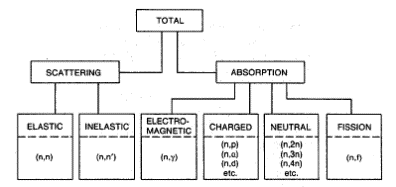
\includegraphics[scale=0.5]{img/image1.png}
			\captionof{figure}{Dipôle}
		\end{wrapfigure}
		Tout élément possède un certain nombre de \textit{bornes} (caractérisée par un potentiel électrique et une valeur de courant\footnote{Lorsque $I$ est identique aux deux bornes, on peut les associer et parler de \textbf{port} ou \textbf{accès}. Le dipôle est par définition un accès.}) qui servent à établir des connexions, un dipôle est simplement un élément en possédant deux.
		
		\subsection{Noeuds, bornes, connexion}
		\begin{wrapfigure}[9]{l}{6cm}
			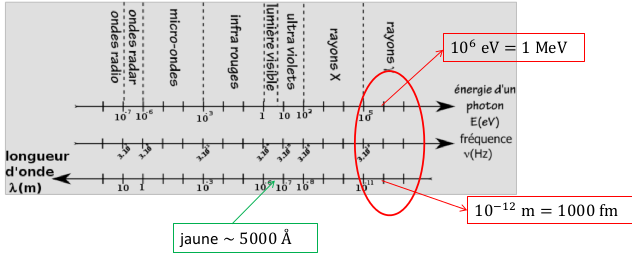
\includegraphics[scale=0.5]{img/image2.png}
			\captionof{figure}{Nœud}
		\end{wrapfigure}
		On connecte les éléments par des bornes : lorsqu'on connecte plusieurs éléments ensemble on forme un noeud, qui est par définition équipotentiel.\\
		\textbf{Attention !} Le noeuds couvre l'ensemble de la connexion et pas seulement le point de contact des fils.\\
		
		Tout dipole ou assemblage de dipole en série constitue une \textbf{branche} est l'ensemble de ces branches constituant un parcours fermé constitue une \textbf{maille}.
		
		\section{Le modèle de Kirchhoff}
		Un circuit à éléments concentrés est un circuit dont les dimensions sont suffisamment petites par rapport à la longueur d'onde de variation des champs pour que l'on puisse y considérer que les phénomènes électromagnétiques s'y propage instantanément (pas besoin de la théorie des champs). On peut dès lors utiliser le \textbf{modèle de Kirchhoff} et ne tenir compte que de la topologie du circuit.
		
		\subsection{Critère de validité du modèle de Kirchhoff}
		Le critère de validité du modèle est le suivant :\\
		
		\prop{La plus grande dimension du circuit est beaucoup plus petite que la longueur d'onde du signal de plus haute fréquence.}\ \\
		Cela revient à dire que $l_{max} << \lambda_{min}$ où $\lambda = \dfrac{c}{f}$.\footnote{Exemples page 11}
		
		\subsection{Les circuits comme cas particuliers de système}
		Non vu au cours, voir page 11.
		
		\subsection{Lois de Kirchhoff}
		\begin{itemize}
			\item[Loi des noeuds] : la somme (algébrique) des courants sortant d'un noeud est nulle
			\item[Loi des mailles] : la somme (algébrique) des tensions le long d'une maille est nulle.
		\end{itemize}
		
		\section{Sens de lecture, charge et source}
		\subsubsection{Sens de lecture}
		Celui-ci correspond au sens de propagation de l'information et en toute généralité, on le "lit" de gauche à droite (entrée à gauche, sortie à droite).
		
		\subsubsection{Charge}
		La charge\footnote{Ne pas confondre avec la charge électrique en coulomb !} (d'un montage) est le composant connecté à l'aval (la sortie) de ce montage. Par exemple, tout appareil connecté à une prise est une charge pour cette prise.
		
		\subsubsection{Montage à vide >< Montage en charge}
		Le circuit fonctionne à vide lorsqu'aucune charge ne lui est connecté, alors que inversement, il sera dit chargé.\\
		\textbf{Attention !} Le montage à vide ne se comporte pas de la même façon que le montage en charge. En effet :\\
		\prop{Connecter un composant additionnel à un circuit revient à modifier ce circuit, et donc potentiellement à redistribuer tous les courants et les tensions dans celui-ci.}\ \\
		
		Plus simplement : \\
		\prop{La tension de sortie d'un montage peut varier en fonction de la charge qui lui est connectée.}
		
		\subsubsection{La source}
		La source (d'un montage) désigne le composant ou l'équipement connecté à l'amont (à l'entrée) de ce montage. Par exemple, un micro envoyant une information à une table est une source.
		
		
		\section{Courant}
		Le \textbf{courant} est un déplacement d'ensemble de charges électriques dans un conducteur.\\
		Notons qu'un courant est généralement constitué d'électrons mais que ce-dernier peut également être constitué d'électrolytes ou de semi-conducteurs.
		
		\subsubsection{Intensité = valeur du courant électrique}
		L'\textbf{intensité} est le débit de charge électrique :
		\begin{equation}
		i(t) = \frac{dq(t)}{dt}
		\end{equation}
		
		\subsubsection{Mesure du courant électrique}
		Il faut insérer un ampèremètre \textbf{en série} avec le fil dans lequel on désire mesurer le courant.
		
		\subsubsection{Représentation du courant : sens conventionnel}
		\begin{wrapfigure}[5]{l}{3.5cm}
			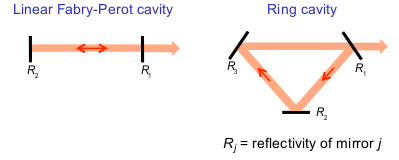
\includegraphics[scale=0.5]{img/image3.png}
			\captionof{figure}{Inversion du sens}
		\end{wrapfigure}
		Il s'agit d'une flèche qui pointe dans la direction de charge qui seraient positives : il s'agit du sens de courant conventionnel qui est toujours représenté dans les schéma.\\
		Si le courant était négatif, on peut le rendre positif en inversant le sens de la flèche.
		
		\subsubsection{Circulation du courant en boucle fermée}
		"Un chemin de retour" doit toujours exister. Branche interrompue : courant nul.
		
		\section{Tension(s)}
		\subsection{La tension : un terme ambigu}
		C'est un terme ambigu car il peut être trois chose distinctes : la force électromotrice, le potentiel d'un noeud ou la d.d.p.
		
		\subsection{DDP et potentiel}
		\subsubsection{Différence de potentiel}
		C'est ce qui se mesure en pratique (à l'aide d'un multimètre, sur un dipôle), il s'agit de la différence de potentiel entre deux bornes.
		
		\subsubsection{Potentiel électrique (première approche)}
		C'est une notion purement théorique qui se résume à dire que le potentiel électrique en un point est l'énergie à dépenser pour amener une charge unitaire depuis un point ou le potentiel est nul (à l'infini).
		
		\subsection{Convention et signes}
		\subsubsection{Convention concernant le sens de la différence de potentiel}
		La ddp étant une soustraction, il faut définir le sens de celle ci.
		Lorsque la flèche va de $B$ vers $A$ (convention) :
		\begin{equation}
		V = V_A - V_B
		\end{equation}
		Ceci découle de cette opération "soustraction", la pointe de la flèche pointera vers le potentiel le plus haut.
		
		\subsection{Interprétation des notions de potentiel et de masse}
		\subsubsection{Potentiel et masse = notion théorique}
		Plus utile que le potentiel, on utilise la masse:\\
		\prop{La masse est le noeud dont le potentiel, par convention, est nul : $V_{masse} = 0V$}\ \\
		
		C'est un choix arbitraire, une convention qui servira de référence.
		Si on connait toutes les ddp, il faut un "repère" sans quoi on ne pourra jamais connaître les potentiels des noeuds (qui est "défini à une constante près").
		
		\subsubsection{Présence/absence de masse}
		On n'a pas besoin de masse pour résoudre un circuit sur papier.\\
		\prop{Si l'on ne s'intéresse qu'aux ddps, il n'est pas nécessaire de définir une masse}\ \\
		
		\subsection{Potentiel représenté comme une ddp}
		\prop{La ddp entre un noeud A quelconque et la masse est numériquement égale au potentiel de ce noeud A}\ \\
		
		\subsection{Tension différentielle}
		Souvent, en présence de masse, on calcule la ddp par rapport avec celle-ci. Si la masse n'est pas présente on parlera de \textbf{tension différentielle} pour bien différencier les deux.
		
		\subsection{Terre = protection}
		\begin{wrapfigure}[5]{r}{2.5cm}
			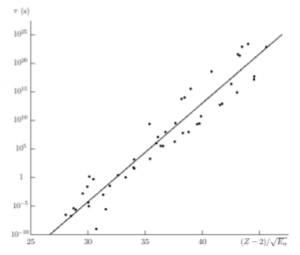
\includegraphics[scale=0.5]{img/image4.png}
			\captionof{figure}{Symboles}
		\end{wrapfigure}
		Il ne faut pas confondre les deux, la terre est une notion pratique relative à la sécurité des personnes et des équipements.
		
		\section{Puissane instantanée, conventions et passivité}
		\subsection{Dipôles actifs et passif - définition intuitive.}
		\begin{itemize}
			\item[Passif] : Ne peut qu'absorber l'énergie (résistance, condensateur, ...)
			\item[Actif] : Injecte de l'énergie dans le circuit (source de tension, pile, ...)
		\end{itemize}
		
		\subsection{Puissance instantanée sur un dipôle}
		La puissance électrique est l'énergie fournie ou reçu par unité de temps par un dipôle
		\begin{equation}
		p(t) = v(t).i(t)
		\end{equation}
		
		\subsection{Conventions récepteurs et générateur}
		Dans tout dipôle passif, les flèches courant et tension doivent être de sens opposés : \textbf{convention récepteur}.\\
		\begin{wrapfigure}[8]{r}{3cm}
			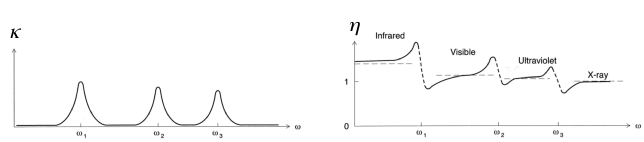
\includegraphics[scale=0.5]{img/image5.png}
			\captionof{figure}{Conv. générateur}
		\end{wrapfigure} Dans cette convention, la formule $p(t)$ donne la puissance instantanée absorbée par ce dipôle.
		
		Dans la source par contre, ces deux flèches doivent être dans le même sens. La formule de puissance donnera dans ce cas la puissance instantanée fournie grâce à la \textbf{convention générateur}.Le rôle de la source est de "relever" le potentiel.
		
		\subsection{Critère de passivité}
		\begin{equation}
		w(t) = \int_0^\infty p(t)dt \geq 0
		\end{equation}
		Un dipôle passif ne peut pas délivrer ce qu'il n'a pas reçu, cela ne peut donc pas être négatif. Si c'est le cas, le dispositif sera \textit{actif}.
		
		\chapter{Dipôles idéaux}
		
		\section{Comportement externe : loi et caractéristique d'un dipôle}
		\subsection{Etat électrique d'un dipôle}
		Il s'agit du couple $(I,V)$ de valeurs électriques mesurables sur un dipôle à l'instant $t$.
		
		\subsection{Comportement électrique du dipôle}
		Les valeurs que prennent $I$ et $V$.
		
		\subsection{Loi du dipôle}
		C'est la formule exprimant mathématiquement le comportement.
		\begin{itemize}
			\item[Source de tension idéale] : $V = E$ : impose une ddp et ce peu importe le courant qui la traverse (ne modifie par le courant).
			\item[Source de courant idéale] : $I = J$ : impose un courant et ce peu impporte la tension (ne modifie pas la tension).
		\end{itemize}
		
		\subsection{Caractéristique}
		La \textbf{caractéristique} est la représentation graphique du \textit{comportement électrique} du dipôle.\footnote{La caractéristique n'apporte aucune info supplémentaire par rapport à la loi.}
		
		\setcounter{section}{2}
		\section{Charges idéales : trois effets physiques}
		\setcounter{subsection}{1}
		\subsection{Inductance}
		La loi de base est que $\phi \propto I$ impliquant :
		\begin{equation}
		\phi (t) = LI
		\end{equation}
		Comme $v(t) = \frac{d\phi}{dt}$ on peut dire que $v(t) = L\frac{di}{dt}$ et $e(t) = -\frac{d\phi}{dt}$ qui est une autre manière d'exprimer la loi de Lenz. On utilisera :
		\begin{itemize}
			\item loi de l'inductance : convention récepteur
			\item loi de Lenz : convention générateur
		\end{itemize}
		
		\begin{center}
			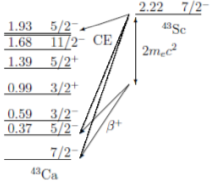
\includegraphics[scale=0.5]{img/image10.png}
			\captionof{figure}{Inductance/Lenz}
		\end{center}
		
		La loi courant-tension décrite ci-dessus implique :
		\begin{itemize}
			\item si la ddp est \textbf{constante}, le courant croît \textbf{linéairement}
			\item si le courant est \textbf{constant}, la ddp est \textbf{nulle}.
		\end{itemize}
		
		
		\subsubsection{Lois "court terme" et "long terme"}
		Dans une self, le courant ne peut pas varier instantanément sinon la ddp serait infinie. Il s'agit de la loi à court terme.\\
		Cependant, après un temps infini la ddp doit forcément être nulle sans quoi $I = - \infty$ ce qui est impossible. Il s'agit de la loi à long terme.
		
		\subsubsection{Interprétation physique}
		Lorsque 'lon essaye de faire varier le courant dans une self, celle-ci développe une fem qui contre cette variation. La self oppose donc une certaine \textit{inertie} à la variation du courant qui la traverse.\\
		
		Histoire de ne pas l'oublier (et de mettre en avant cet "effet mémoire"), voici la loi courant tension de la self:
		\begin{equation}
		i(t) = i(0) + \frac{1}{L}\int_0^t v(t) dt
		\end{equation}
		
		
		\subsection{Capacité}
		La loi de base à retenir est que $Q \propto V$.
		\begin{equation}
		i(t) = C \frac{dv(t)}{dt}
		\end{equation}
		où $v$ est la ddp. On dira que
		\begin{itemize}
			\item la capa se \textbf{charge} quand la ddp (ou |Q|) \textbf{augmente}
			\item la capa se \textbf{décharge} quand la ddp (ou |Q|) \textbf{diminue}
		\end{itemize}
		
		
		\subsubsection{Interprétation physique}
		A cause de la dérivée dans cette expression on remarque, à l'inverse de $R$\footnote{Où courant implique tension}, que c'est la \textit{variation de la ddp} qui implique l'existence d'un courant et inversement.\\
		Une capacité n'a pas de caractéristique dans le plan $(I,V)$ car le temps y intervient. Retenons que
		\begin{enumerate}
			\item si le courant est constant, la ddp croit linéairement
			\item si la ddp est constante, le courant est nul.
		\end{enumerate}
		
		\subsubsection{Lois "court terme" et "long terme"}
		On constante que la $ddp$ ne varie pas instantanément sinon $i(t) = \infty$ ce qui est impossible.\\
		Après un temps infini, le courant doit forcément être nul sinon la ddp atteindrait une valeur négative infinie ce qui est également impossible.
		
		\subsubsection{Autre interprétation physique}
		Pour faire varier la charge, il faut injecter ou retirer des charges à la capacité, ce qui prends un certain temps (pas instantané): il faut qu'un courant circule : on dit que la capacité s'\textbf{oppose/présente une inertie} aux variations de tension
		
		\subsubsection{Charge initiale}
		La loi de base exprimée en tension et en courant est 
		\begin{equation}
		v(t) = \frac{1}{C} \int_{-\infty}^t i(t) dt
		\end{equation}
		Ou encore, plus pratiquement (ne pas oublier $v(0)$ qui traduit un "effet de mémoire" :
		\begin{equation}
		v(t) = v(0) + \frac{1}{C} \int_0^t i(t) dt
		\end{equation}
		
		
		
		
		
		
		
		\setcounter{section}{6}
		\section{Court-circuit et circuit ouvert (Examen!!)}
		\subsection{Court-circuit}
		Il s'agit d'un dipôle imposant une ddp nulle, quelque soit la valeur du courant qui le traverse : $V = 0$.\\ On réalise un court circuit en mettant deux noeuds au même potentiel.
		\textbf{Attention !} Ddp nulle n'implique pas que le courant l'est également !
		
		\subsection{Circuit ouvert}
		Un \textbf{circuit ouvert} est par définition un dipôle traversé par un courant nul, quelque soit la ddp à ses bornes : $I =0$.\\
		\textbf{Attention !} Encore une fois, la ddp aux bornes d'un circuit ouvert est à priori \textbf{non} nulle !
		
		\setcounter{section}{8}
		\section{Modélisation d'un élément/dispositif réel par schéma équivalent}
		Chaque composant réel étant complexe et non-idéal, il devra être modélisé par un schéma équivalent, c'est-à-dire un assemblage d'éléments idéaux (qui n'existent donc \textbf{pas} en réalité).
		
		
		\chapter{Quadripôles idéaux}
		\setcounter{section}{2}
		\section{Inductance mutuelle et transformateur idéal}
		\subsection{Phénonmène d'induction mutuelle}
		Le transformateur exploite le phénomène d'induction mutuelle entre deux enroulements (loi de Lenz).\\
		On parle d'induction mutuelle (et pas self-induction) lorsque l'origine du flux magnétique induisant une f.e.m. dans une spire est un courant dans une autre spire.
		\begin{equation}
		e_1 = -\frac{d\phi_1}{dt}\ \ \ \ \ \ \ \ \phi_1 = M_{12}i_2\ \ \ \ \ \ \ \ V_1 = \pm M\frac{di_2}{dt}
		\end{equation}
		Le facteur $M_{12}$ est le coefficient d'inductance mutuelle entre les deux spires.
		
		\subsection{Quadripôle "transformateur"}
		\begin{wrapfigure}[8]{r}{3cm}
			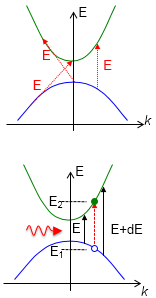
\includegraphics[scale=0.5]{img/image18.png}
			\captionof{figure}{Transformateur}
		\end{wrapfigure}
		Soit deux spire parcourues par un courant : chacune capte son flux "propre" et un flux mutuel :
		\begin{equation}
		\left\{\begin{array}{l}
		\Phi_1 = L_1i_1 + Mi_2\\
		\Phi_2 = Mi_1 + L_2i_2
		\end{array}\right.
		\end{equation}
		En tension, on peut écrire ces lois $\left\{\begin{array}{l}
		v_1(t) = L_1\frac{di_1}{dt} + M\frac{di_2}{dt}\\
		v_2(t) = M\frac{di_1}{dt} + L_2\frac{di_2}{dt}
		\end{array}\right.$
		
		\subsubsection{Signe du terme d'inductance mutuelle (en conventions récepteur}
		\begin{wrapfigure}[8]{L}{5cm}
			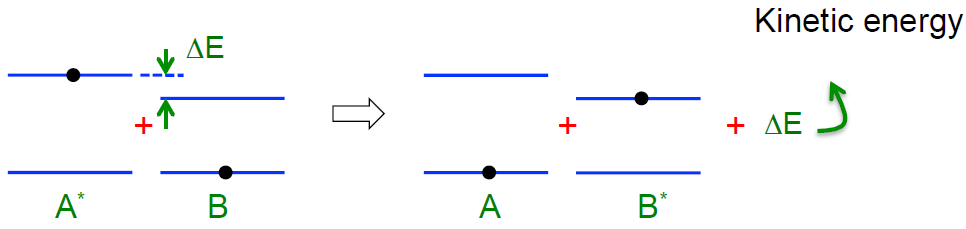
\includegraphics[scale=0.3]{img/image19.png}
			\captionof{figure}{Signe du couplage}
		\end{wrapfigure}
		Avant tout, deux situations peuvent exister : 
		\begin{enumerate}
			\item La fem mutuelle est de même sens que la fem propre : on les additionne
			\item La fem mutuelle est de sens opposé : on les soustrait
		\end{enumerate}
		Par exemple, regardons la \textsc{Figure 3.2} :
		\begin{itemize}
			\item Le courant $i_1$ entre par la borne $A$ et crée dans le noyau un flux $\phi_1$ dirigé vers la gauche
			\item Le courant $i_2$ entre par la borne $D$ et crée dans le noyau un flux $\phi_2$ dirigé vers la gauche
			\item Les deux flux sont dans le même sens et donc s'additionne
		\end{itemize}
		Le couplage (positif ou négatif, ici positif) dépend donc de la position géométrique des bobines et des conventions utilisées pour définir les courants.\\
		
		Pour tenir compte de la disposition spatiale des enroulements on place des "points" qui indiquent que le signe donner au terme d'inductance mutuelle en fonction des sens du courant sur le quadripôle. Ils sont définis :
		\begin{itemize}
			\item Couplage positif (+M) si les positions relatives du point et du sens de courant conventionnel sont identiques pour les deux spires
			\item Couplage négatif (-M) si les positions relatives du point et du sens du courant conventionnel sont opposées pour les deux spires
		\end{itemize}\ \\
		
		Ceci bien sur sous hypothèses que $M$ est positif et que la convention récepteur est définie sur chaque spire (si convention générateur, inverser les signes des équations de la spire, ou changer le sens du courant concerné)\footnote{Exemple page 95-97}.
		
		\setcounter{subsection}{2}
		\subsection{Résolution de circuits comprenant un transformateur}
		Un exemple de résolution est donné slide 85-90.
		
		\subsection{Puissance et énergie absorbées par le transformateur}
		La puissance instantanée absorbée par un quadripôle vaut la somme des puissances instantanées aux deux accès (conv. recept.)
		\begin{equation}
		p(t) = v_1(t).i_1(t) + v_2(t).i_2(t)
		\end{equation}
		L'énergie absorbée correspond à l'intégrale de cette puissance bornée de $-\infty$ à $t$ ce qui donne :
		\begin{equation}
		\frac{1}{2}L_1i^2_1(t) + Mi_1(t)i_2(t) + \frac{1}{2}L_2i_2^2(t)
		\end{equation}
		
		
		\subsection{Association d'enroulements couplés}
		Lorsque deux enroulements sont couplés en série ou en parallèle, ils forment un dipôle.
		\subsubsection{Association en série (couplage positif, même courant)}
		\begin{proof}
			L'inductance du dipôle vaut par définition $v = L_{eq}\frac{di}{dt}$. Avant la connexion, les enroulement formaient un quadripole (transformateur) :
			\begin{equation}
			\left\{\begin{array}{l}
			v_1(t) = L_1\frac{di_1}{dt} + M \frac{di_2}{dt}\\
			v_2(t) = M\frac{di_1}{dt} + L_2 \frac{di_2}{dt}
			\end{array}\right.
			\end{equation}
			La connexion en série permet d'écrire que $i_1 = i_2$ ainsi que $v = v_1 + v_2$. On obtient donc :
			\begin{equation}
			v = (L_1 + L_2 + 2M)\frac{di}{dt}
			\end{equation}
		\end{proof}
		Par identification, on peut dire que $L_{eq} = L_1 + L_2 + 2M$.\\
		
		Si le couplage est négatif, le signe de la mutuelle $M$ devient négatif et la relation (démonstration équivalente) devient :
		\begin{equation}
		v = (L_1 + L_2 - 2M)\frac{di}{dt}
		\end{equation}
		
		\subsubsection{Association en parallèle}
		Lorsque deux enroulement sont connectés en parallèle selon un couplage positif, l'inductance équivalente vaut :
		\begin{equation}
		L_{eq} = \frac{L_1L_2-M^2}{L_1+L_2-2M}
		\end{equation}
		\begin{proof}
			Avant la connexion, les enroulement formaient un quadripole (transformateur) :
			\begin{equation}
			\left\{\begin{array}{l}
			v_1(t) = L_1\frac{di_1}{dt} + M \frac{di_2}{dt}\\
			v_2(t) = M\frac{di_1}{dt} + L_2 \frac{di_2}{dt}
			\end{array}\right.
			\end{equation}
			La connexion en parallèle permet d'écrire que $i = i_1 + i_2$ ainsi que $v = v_1 = v_2$.\\
			
			En soustrayant les deux équations du quadripôle :
			\begin{equation}
			v_1 - v_2 =(L_1-M)\frac{di_1}{dt} + (M-L_2)\frac{di_2}{dt} = 0
			\end{equation}
			Après avoir fait le ménage :
			\begin{equation}
			\frac{di_2}{dt} = \left(\frac{M-L_1}{M-L_2}\right)\frac{di_1}{dt}
			\end{equation}
			Grâce à la loi de mailles énoncée ci-dessus, ($di/dt = di_1/dt + di_2/dt$) on trouve en remplaçant :
			\begin{equation}
			\frac{di}{dt} = \left(1+\frac{M-L_1}{M-L_2}\right)\frac{di_1}{dt}
			\end{equation}
			Et finalement : 
			\begin{equation}
			L_{eq} = \frac{L_1L_2-M^2}{L_1+L_2-2M}
			\end{equation}
		\end{proof}
		Pour un couplage négatif (sens de $L_2$ inversé), il suffit d'inverser le signe de $M$. On obtient dès lors :
		\begin{equation}
		L_{eq} = \frac{L_1L_2-M^2}{L_1+L_2+2M}
		\end{equation}
		
		\subsection{Transformateur idéalement couplé}
		Certains transformateurs sont encore plus idéaux que d'autres. La meilleure situation est celle ou l'intégralité du flux généré par un enroulement est capté par l'autre. Dans ce cas\footnote{Démonstration dans la théorie des champs} :
		\begin{equation}
		M^2 = L_1L_2
		\end{equation}
		Dans ce cas, le rapport des tension vaut le rapport des spires :
		\begin{equation}
		\frac{v_2(t)}{v_1(t)} = \frac{N_2}{N_1} = \sqrt{\frac{L_1}{L_2}}
		\end{equation}
		On peut écrire les tension (et les courants, en sens inverse) : 
		\begin{equation}
		\left\{\begin{array}{l}
		v_2(t) = \frac{N_2}{N_1}v_1(t)\\
		i_2(t) = -\frac{N_2}{N_1}i_1(t)
		\end{array}\right.
		\end{equation}
		Ce qui peut se simplifier en :
		\begin{equation}
		\left\{\begin{array}{l}
		v_1(t) = nv_2(t)\\
		i_2(t) = ni_1(t)
		\end{array}\right.
		\end{equation}
		où $n = \frac{N_1}{N_2}$ est le rapport de transformation.
		
		
		
		\section{Caractérisation des biportes}
		\subsection{Introduction}
		Pour rappel, un biporte n'est rien d'autre qu'un quadripôle. Les circuits extérieurs qui se connectent au biporte définissent deux relations entre ces quatre grandeurs : les \textit{relations constitutives}\footnote{Elles définissent le comportement électrique du biporte vis-à-vis de l'extérieur.}.\\
		\begin{wrapfigure}[8]{r}{3cm}
			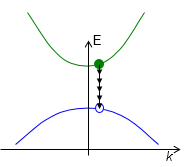
\includegraphics[scale=0.5]{img/image30.png}
			\captionof{figure}{Biporte}
		\end{wrapfigure}
		Plusieurs hypothèses sont faites :
		\begin{enumerate}
			\item Le courant entrant par une borne d'accès est égal à celui qui ressort par l'autre borne du même accès.
			\item Pas de sources indépendantes dans le biporte
			\item Utilisation des références associées (= convention récepteur)
			\item On s'intéresse aux 4 grandeurs $\underline{V_1}, \underline{V_2}, \underline{I_1}$ et $\underline{I_2}$.
		\end{enumerate}
		Pour résoudre un tel circuit, on utilise la procédure standard en écrivant les équations du circuit.\\
		
		Revenons aux deux relations constitutives entre les quatre grandeurs aux accès. On a donc six possibilités pour exprimer deux grandeurs en fonction des deux autres $\rightarrow$ six matrices possibles.\\
		Le but du chapitre est de voir "quel cas convient le mieux"\footnote{Je ne fais ici que la matrice impédance, pour le reste \textit{Cf. slides 70 - 97, syllabus page 105}}.
		
		\subsection{Matrice impédance}
		La matrice impédance est une généralisation de l'impédance en 2D. Elle permet d'exprimer les tensions en fonctions des courants. Ainsi $\underline{V} = Z\underline{I}$ devient :
		\begin{equation}
		\left[\begin{array}{l}
		\underline{V_1}\\
		\underline{V_2}
		\end{array}\right] = \left[\begin{array}{c c}
		z_{11}(j\omega) & z_{12}(j\omega)\\
		z_{21}(j\omega) & z_{22}(j\omega)
		\end{array}\right]\left[\begin{array}{l}
		\underline{I_1}\\
		\underline{I_2}
		\end{array}\right]
		\end{equation}
		Ce qui est équivalent à :
		\begin{equation}
		\left\{\begin{array}{l}
		\underline{V_1} = z_{11}(j\omega)\underline{I_1} + z_{12}(j\omega)\underline{I_2}\\
		\underline{V_2} = z_{21}(j\omega)\underline{I_1} + z_{22}(j\omega)\underline{I_2}
		\end{array}\right.
		\end{equation}
		
		
		
		
		
		
		
		
		
		
		
		
		
		
		
		
		
		
		\chapter{Équivalence de Thévenin et adaptation d'impédance}
		Ce n'est pas parce que deux composants électriques fonctionnent séparément que ce sera toujours le cas en les connectant ensemble. \\
		La notion d'équivalent de Thévenin permet de prédire si un assemblage de deux circuits va "fonctionner" (oopas).
		
		
		\section{Circuits équivalents et théorèmes de Thévenin/Norton}
		\subsection{Équivalence de deux circuits}
		\prop{Deux circuits sont équivalents (au sens de Thévenin) s'ils ont la même caractéristique}\ \\
		
		Comme la caractéristique traduit le comportement aux bornes du circuit, cela revient à dire que :\\
		\prop{Deux circuits sont équivalents s'ils possèdent le même comportement électrique (vu du circuit extérieur)}\ \\
		
		En régime sinusoïdal, deux dipôles seront équivalent s'ils ont la même impédance.
		
		
		\subsection{Théorème et équivalent de Thévenin}
		Le \textbf{théorème de Thévenin} s'énonce :\\
		
		\prop{Tout circuit linéaire et permanent est équivalent à une source de tension unique $V_{th}$ en série avec une impédance $Z_{th}$.}
		\begin{center}
			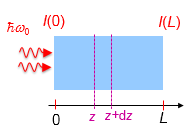
\includegraphics[scale=0.7]{img/image21.png}
			\captionof{figure}{Illustration du théorème de Thévenin}
		\end{center}
		Notons que $V_{th}$ est la tension à vide (ou fem à vide) entre les bornes du réseau (ici $d$ lorsque celui-ci est déconnecté de tout autre réseau. 
		$Z_{th}$ est l'impédance, vue des bornes du réseau.
		
		
		\subsection{Théorème et équivalent de Norton}
		Le \textbf{théorème de Norton} est une variante du th. de Thévenin, utilisant cette fois une source de courant :\\
		\prop{Tout réseau linéaire et permanent est équivalent à une source de \textit{courant} unique $I_N$ en \textit{parallèle} avec une impédance $Z_N$.}
		\begin{center}
			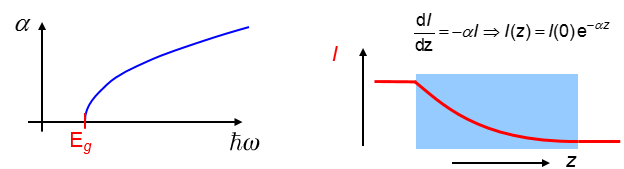
\includegraphics[scale=0.7]{img/image22.png}
			\captionof{figure}{Illustration du théorème de Norton}
		\end{center}
		
		
		Une multitude d'exemples d'applications sont disponibles dans les slides (24-31)\\
		Les démonstrations de ces théorèmes sont à connaître (slide 31 et page 127-128).
		
		\section{Impédance d'entrée, impédance de sortie}
		\subsection{Équivalent de Thévenin d'un dipôle charge : résistance d'entrée}
		Supposons qu'un appareil (une charge) doivent recevoir une tension à ses bornes. S'il est linéaire, il lui correspond un équivalent de Thévenin possédant le même comportement électrique.\\
		
		Pour se faire, on définit la \textbf{résistance d'entrée} $R_{in}$ d'un dipôle charge linéaire comme la valeur de la résistance équivalente (au sens de Thévenin) à ce dipôle. Autrement dit :
		\begin{itemize}
			\item La valeur de la résistance de l'équivalent de Thévenin du dipôle
			\item L'inverse de la pente de la caractéristique de ce dipôle
			\item La résistance par laquelle on peut remplacer ce dipôle sans modifier le fonctionnement du circuit extérieur
		\end{itemize}\ \\
		\prop{La résistance d'entrée est avant tout un \textit{nombre} caractérisant le comportement externe du dipôle ([$\Omega$])}\ \\
		Ce n'est donc \textbf{PAS} (sauf exception rare) la résistance qui se trouve à l'entrée du circuit !
		\subsubsection{Interprétation}
		Si un dipôle possède une résistance d'entrée de $500\Omega$ cela signifie simplement que si on lui applique une tension de $10V$ il consommera comme courant $20 mA$.\\
		
		Cette notion permet de remplacer, du point de vue du circuit extérieur, un montage complexe par une résistance fictive unique.
		
		\subsection{Équivalent de Thévenin d'un dipôle source : résistance de sortie et fem à vide}
		Pour autant que le circuit soit linéaire, il peut être modélisé par un circuit équivalent de Thévenin. Définissons :
		\begin{description}
			\item[Résistance de sortie] ; Valeur de la résistance de l'équivalent de Thévenin de ce dipôle.
			\item[Fem à vide] ; Valeur de la source de tension idéale de l'équivalent de Thévenin de ce dipôle.
		\end{description}
		
		\subsubsection{Interprétation}
		\begin{wrapfigure}[8]{r}{3cm}
			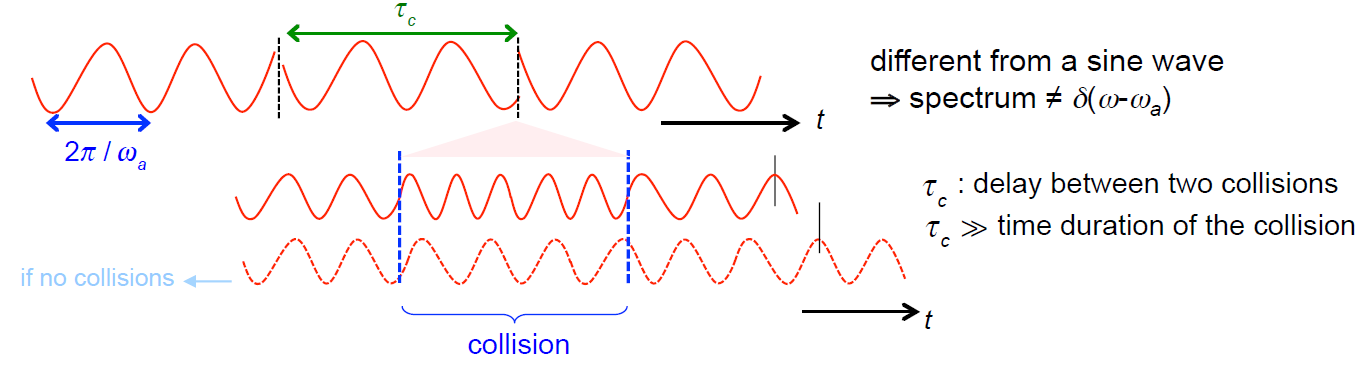
\includegraphics[scale=0.4]{img/image20.png}
			\captionof{figure}{Influence de la résistance de sortie}
		\end{wrapfigure}
		La \textit{fem à vide} est la valeur de la tension visible à la sortie du dipôle lorsque celui-ci ne délivre aucun courant. La tension à la sortie du dipôle valant (dans ce cas $I = 0A$) :
		\begin{equation}
		V = e_{out} - R_{out}I
		\end{equation}
		Cette équation permet également de comprendre la \textit{résistance de sortie}. Lorsqu'un courant passe, la résistance de sortie introduit une certaine chute de tension. La tension de sortie est donc plus basse que la fem à vide.\\
		
		\prop{La résistance de sortie traduit la difficulté du dipôle à maintenir sa tension de sortie constante lorsque le courant délivré augmente.}
		
		
		\setcounter{subsection}{3}
		\subsection{Équivalent de Thévenin/Norton d'un quadripôle}
		\begin{wrapfigure}[8]{l}{4.7cm}
			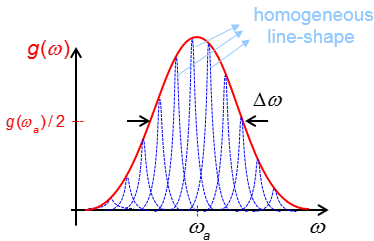
\includegraphics[scale=0.3]{img/image23.png}
			\captionof{figure}{Equivalent de Thévenin d'un quadripôle}
		\end{wrapfigure}
		Il suffit de modéliser l'entrée et la sortie par un équivalent de Thévenin comme précédemment. L'appareil sera caractérisé lors de la connaissances de trois paramètres :
		\begin{enumerate}
			\item Sa résistance d'entrée $R_{in}$
			\item Sa résistance de sortie $R_{out}$
			\item Sa fem à vide ($e_{out}$)
		\end{enumerate}
		Il existe bien entendu cette fois une tension d'entrée, de sortie et même chose pour le courant.
		
		
		\section{Adaptation d'impédance}
		\subsection{Connecter deux appareils : pas si simple !}
		Soit le cas ou on souhaite connecter un apareil en "amont" (source délivrant un signal) à un appareil en "aval" (charge recevant ce signal)\footnote{Chacun de ces appareils sont typiquement des quadripôles.}. Un principe de base est à retenir :\\
		\prop{On \textbf{ne} peut \textbf{pas} interconnecter des composants et des montages sans effectuer certaines \textit{vérification}.}\ \\
		
		Il faut :
		\begin{enumerate}
			\item Vérifier que l'appareil en aval supporte les niveaux de tensions délivrés par l'appareil en amont (risque de dommages)
			\item Vérifier l'\textbf{adaptation d'impédance}, c'est-à-dire que les résistance d'entrée et de sortie sont "compatibles".\footnote{On pourrait sinon "bloquer" une grande partie du signal.} Ces critères diffèrent suivant que l'on veut transmettre une tension, un courant ou une puissance.
		\end{enumerate}
		
		\subsection{Adaptation d'impédance en tension}
		Si l'on connecte deux appareil (modélisés par leur équivalent de Thévenin), on modifie la tension présente à l'entrée de l'appareil en aval (gauche) qui ne vaut plus $e$ : formule du diviseur résistif :
		\begin{equation}
		\left\{\begin{array}{l}
		I = \frac{E}{R_{in} + R_{out}}\\
		V = R_{in} I
		\end{array}\right.
		\end{equation}
		et donc : 
		\begin{equation}
		V = \frac{R_{in}}{R_{in} + R_{out}}e
		\end{equation}
		\begin{wrapfigure}[5]{l}{5.5cm}
			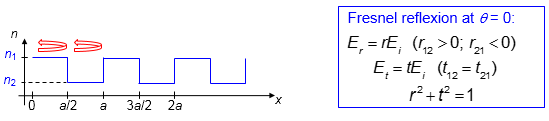
\includegraphics[scale=0.3]{img/image24.png}
			\captionof{figure}{Adaptation d'impédance en tension}
		\end{wrapfigure}
		Le signal de l'appareil en amont est affaibli. Pour éviter toute dégradation, ce "rapport de résistance" doit être proche de l'unité. Le \textbf{critère d'adaptation d'impédance en tension} est donc :\\
		\prop{Lorsqu'on désire transmettre un signal de tension, l'impédance de sortie doit être faible devant l'impédance d'entrée.}
		
		
		\subsection{Adaptation d'impédance en courant}
		Reprenons le cas de figure précédent si ce n'est que l'appareil en amont se comporte comme une \textbf{source de courant}. La sortie de l'appareil en amont est décrite par un équivalent de \textit{Norton}. Calculons le courant reçu  par l'appareil en aval :
		\begin{equation}
		\left\{\begin{array}{l}
		V = R_{in}\\
		V = R_{out}(J-I)
		\end{array}\right.
		\end{equation}
		\begin{wrapfigure}[6]{r}{4.7cm}
			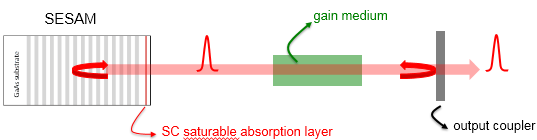
\includegraphics[scale=0.3]{img/image25.png}
			\captionof{figure}{Adaptation d'impédance en courant}
		\end{wrapfigure}
		Le courant dans l'appareil en avant vaut dès lors :
		
		Le signal de l'app
		\begin{equation}
		I = \frac{R_{out}}{R_{in} + R_{out}}J
		\end{equation}
		Cette fois, on trouvera une atténuation aussi faible que possible en suivant le \textbf{critère d'adaptation d'impédance en courant} :\\
		
		\prop{Lorsqu'on désire transmettre un signal de courant, l'impédance d'entrée doit être faible devant l'impédance de sortie.}
		
		\subsection{Adaptation d'impédance en puissance}
		Prenons le cas général ou l'impédance d'entrée $Z_L$ est raccordée à une source de fem vide \underline{$E_S$} et d'impédance interne $Z_S$.\\
		Le but est d'optimiser $Z_L$ ($Z_S$ étant supposé fixe) de façon à maximiser la puissance moyenne qu'elle absorbe, en régime sinusoïdal permanent.\\
		La démonstration page 144 - 145 du syllabus nous donne le critère tant recherché...\\
		
		\prop{Pour maximiser la puissance transmise de la source à la charge, l'impédance de charge doit être le complexe conjugé de l'impédance de source. \begin{equation}
			Z_L = Z^*_S
			\end{equation}}
		
		
		\section{Cas particulier des appareils de mesure}
		\subsection{Connexion d'un appareil de mesure}
		Connecter un \textit{voltmètre} ou un \textit{ampèremètre} dans un circuit, cela revient à le modifier ! Analysons ceci grâce aux sections précédentes.\\
		\begin{center}
			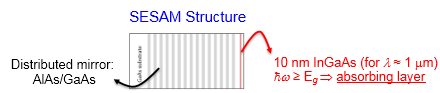
\includegraphics[scale=0.3]{img/image26.png}
			\captionof{figure}{Application de l'équivalent de Thévenin}
		\end{center}
		\textit{Remarque :} Les nœuds choisi pour mesurer une tension (par ex.) ne sont pas forcément des bornes d'entrée/sortie du montage. C'est la encore que l'équivalent de Thévenin va s'appliquer.
		
		\subsection{Nœuds à haute et basse impédance}
		\subsubsection{Impédance d'un nœud}
		\begin{wrapfigure}[6]{r}{3.5cm}
			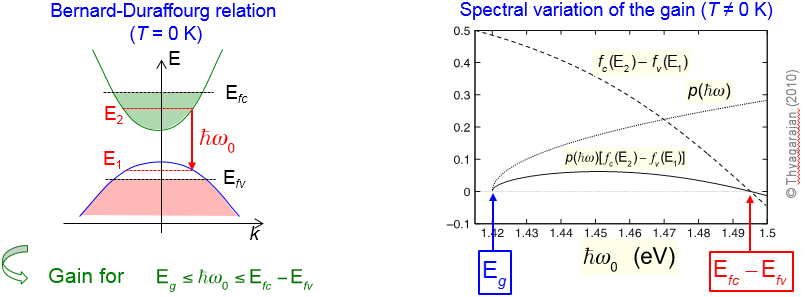
\includegraphics[scale=0.3]{img/image27.png}
			\captionof{figure}{Impédance de nœuds}
		\end{wrapfigure}
		Si l'un des deux nœuds est la masse, le montage est dit \textit{référencé à la masse} (B).\\
		L'\textbf{impédance du nœud A} est la résistance de sortie de l'équivalent de Thévenin du montage.\\
		On parle de noeud à \textit{haute} ou \textit{basse} impédance suivant la valeur de cette résistance de sortie (typiquement autour de $100 k\Omega$).
		
		
		\subsection{Connexion d'un voltmètre}
		\begin{wrapfigure}[6]{l}{4.7cm}
			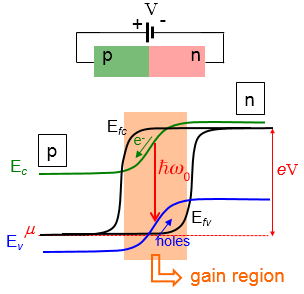
\includegraphics[scale=0.3]{img/image28.png}
			\captionof{figure}{Cas du voltmètre}
		\end{wrapfigure}
		On saura que l'on ne perturbe pas le montage en branchant un voltmètre suivant le critère d'adaptation d 'impédance en tension. Le voltmètre doit avoir \textit{une impédance d'entrée beaucoup plus élevée que l'impédance existant entre les nœuds utilisés pour faire la mesure.}\ \\
		
		\subsection{Connexion d'un ampèremètre}
		\begin{wrapfigure}[6]{r}{4cm}
			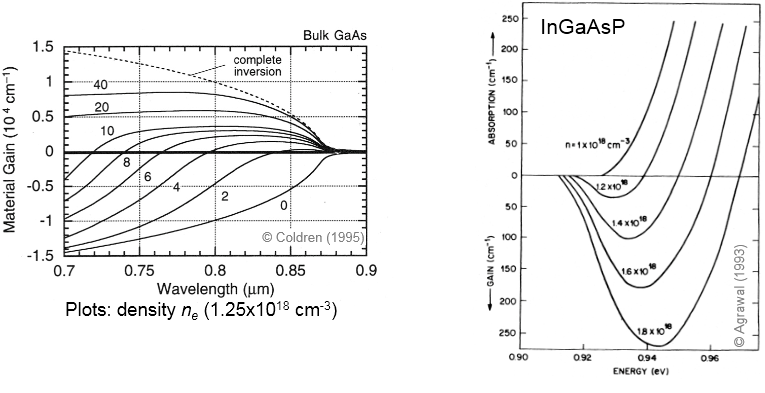
\includegraphics[scale=0.3]{img/image29.png}
			\captionof{figure}{Cas de l'ampèremètre}
		\end{wrapfigure}
		Un  ampèremètre se connecte en \textit{série} pour mesurer un courant, il faut donc obligatoirement interrompre un fil de ce circuit. Il faudra cette fois utiliser un équivalent de Norton. Des résultats précédents, on peut conclure que l'\textit{impédance d'entrée de l'ampèremètre doit être beaucoup plus faible que l'impédance existant entre les nœuds entre lesquels on insère l'ampèremètre}\footnote{Le but est bien d'essayer d'avoir la résistance la plus faible pour se comporter "comme un fil". \textit{Cf. Physique générale - Labo 1}}.
		
		
		
		
		
		
		
		
		
		
		
		
		
		
		
		
		
		
		
		
		
		
		
		
		\chapter{Résoudre un circuit : procédure de base et accélérateurs}
		\section{Vocabulaire lié aux circuits}
		Rappel du premier chapitre.
		
		\section{Lois de Kirchhoff}
		Rappel du premier chapitre.
		
		\section{Procédure canonique en 6 étapes}
		\subsection{Avertissement}
		Cette méthode se base sur les \textbf{courants de branche} qui à l'avantage de considérer des courants réellement mesurable à l'inverse de la méthode des \textbf{courants de maille}.
		
		\subsection{Vue d'ensemble}
		Les six étapes à suivre sont les suivantes :
		\begin{enumerate}
			\item définir une flèche de courant dans chaque branche du circuit
			\item définir sur chaque élément la flèche de tension (ddp) correspondante
			\item exprimer les équations qui lient les tensions (loi des mailles)
			\item exprimer les équations qui lient les courants (loi des nœuds)
			\item exprimer les lois des éléments
			\item résoudre le système d'équation
		\end{enumerate}
		\subsection{Étape 1 : définir une flèche de courant dans chaque branche du circuit}
		On donne un courant par branche, dont le sens (de la flèche) n'est pas importante afin d'identifier clairement de quoi on parle.
		
		\subsection{Étape 2 : définir sur chaque élément la flèche de tension (ddp) correspondant}
		\begin{wrapfigure}[4]{r}{3cm}
			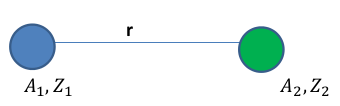
\includegraphics[scale=0.2]{img/image6.png}
			\captionof{figure}{Étape 1, 2}
		\end{wrapfigure}
		On donne une ddp par dipôle en tenant compte du sens du courant (étape 1) ainsi que des conventions récepteurs ou générateurs.\footnote{Cela permet d'éviter de devoir tenir compte des signes}
		
		\subsection{Étape 3 : exprimer les équations qui lient les tensions (loi des mailles)}
		\begin{wrapfigure}[4]{l}{3cm}
			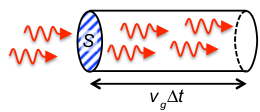
\includegraphics[scale=0.2]{img/image7.png}
			\captionof{figure}{Nœud de départ}
		\end{wrapfigure}
		La somme des tensions le long d'une maille doit être nulle. On choisi premièrement un sens arbitraire de parcours de la maille et un nœud de départ et l'on additionne les potentiels (étape 2). Lorsque l'on retombe sur le nœud de départ on égale la somme obtenue à zéro.
		\begin{equation}
		\left\{\begin{array}{l}
		v_I - v_1 -v_3 = 0\\
		v_3 - v_2 + v_E = 0
		\end{array}\right.
		\end{equation}
		
		\subsection{Étape 4 : exprimer les équations qui lient les courants (lois des nœuds)}
		On fixe un nœud avec plus de deux composantes (sinon déjà défini par l'étape 1) et zou : 
		\begin{equation}
		i_1 - i_2 - i_3 = 0
		\end{equation}
		
		\subsection{Étape 5 : exprimer les lois des éléments}
		Dans notre exemple, pas besoin de réfléchir au signes (de $R$) grâce aux deux précédentes étapes.
		\begin{equation}
		\left\{\begin{array}{l}
		v_1 = R_1i_1\\
		v_2 = R_2i_2\\
		v_3 = R_3i_3\\
		i_1 = I\\
		v_E = - E
		\end{array}\right.
		\end{equation}
		
		\subsection{Étape 6 : résoudre le système obtenu}
		Il nous suffit de trouver $i_2$ et $i_3$ pour ensuite définir toutes les tensions du circuit : celui-ci est résolu !
		
		\subsection{Étape 7 : parfaire la finition}
		\begin{enumerate}
			\item Inverser les signes négatifs
			\item Vérifier la loi des nœuds et des mailles
		\end{enumerate}
		
		\subsection{Étape 0 : boucler les boucles}
		\begin{wrapfigure}[4]{r}{3cm}
			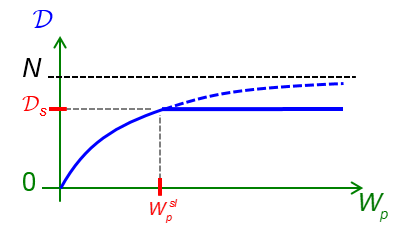
\includegraphics[scale=0.3]{img/image8.png}
			\captionof{figure}{Étape 0}
		\end{wrapfigure}
		Dans certaines représentations rapide, certaines mailles disparaissent. Pour retrouver le "bon" circuit il faut savoir que :
		\begin{itemize}
			\item un nœud isolé (non connecté) à côté duquel figure une valeur de tension représente en fait une source de tension (de cette valeur) entre le nœud et la masse. 
			\item es différentes masses sont implicitement connectée ensemble.
		\end{itemize}
		
		\setcounter{section}{4}
		\section{Équivalence série et parallèle}
		Les deux définitions à retenir sont les suivantes :
		\begin{description}
			\item[En série] : Deux dipôles sont connectés en série ssi ils ont \textit{parcourus par le même courant}.
			\item[En parallèle] : Deux dipôles sont connectés en parallèle ssi ils sont \textit{soumis à la même ddp}.
		\end{description}
		Pour le reste, on connaît les règles !
		
		\section{Utilisation des théorème de Thévenin/Norton pour résoudre un circuit}
		Cette matière sera couverte en laboratoire. \textit{Cf. page 173-175}
		
		\setcounter{section}{7}
		\section{Théorème de superposition}
		\subsection{Énoncé}
		Il s'agit d'un accélérateur pour les circuits \textbf{linéaires}\footnote{$R, C, L = cste$}.\\
		
		\prop{Dans un circuit linéaire contenant \textbf{plusieurs sources} on peut calculer le circuit pour chacune des sources \textbf{comme si elle était seule}, puis sommer toutes les contributions de tension et de courant ainsi obtenues pour trouver le résultat final.}
		
		\subsection{Exemple d'application}
		On supprime ainsi toutes les sources sauf une tout en remplaçant :
		\begin{itemize}
			\item les sources de tension par un court-circuit
			\item les sources de courant par un circuit ouvert
		\end{itemize}
		
		\begin{center}
			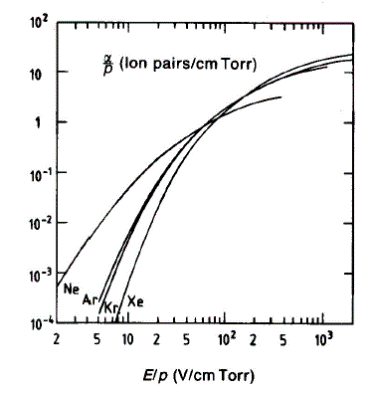
\includegraphics[scale=0.4]{img/image9.png}
			\captionof{figure}{Exemple d'application du théorème de superposition}
		\end{center}
		
		\subsection{Critères d'utilisation en présence de phaseurs}
		Deux cas peuvent se présenter lorsque l'on résous un circuit à plusieurs sources en utilisant les phaseurs : toutes les sources ont la même fréquences, ou non.
		\subsubsection{Même fréquence pour toutes les sources}
		\begin{itemize}
			\item Hypothèses du régime sinusoïdal
			\item On peut utiliser les phaseurs sur le circuit complet
			\item On \textbf{peut} donc :
			\begin{itemize}
				\item Soit résoudre le circuit (par les phaseurs) en considérant simultanément toutes les sources
				\item Soit utiliser le th. de superpo : résoudre séparément chaque sous-circuit (par les phaseurs) puis sommer les réponses (temporelle ou en phaseurs)
			\end{itemize}
		\end{itemize}
		
		
		\subsubsection{Fréquence pour  les sources}
		\begin{itemize}
			\item On n'est \textbf{pas} dans les  hypothèses du régime sinusoïdal et l'on ne peut pas utiliser les phaseurs !!
			\item On \textbf{doit} utiliser la superposition pour utiliser les phaseurs (séparations des différentes fréquences)
			\begin{itemize}
				\item Résoud individuellement les sous-circuits par les phaseurs
				\item \textbf{On ne peut pas sommer les phaseurs}
				\item On \textbf{doit} sommer les réponses temporelles (ou résoudre dès le départ tout en temporel)
			\end{itemize}
		\end{itemize}
		Pour résumer :\\
		
		\prop{
			\begin{enumerate}
				\item Lorsque les sources ne comportent qu'une seule fréquence, on \textit{peut} utiliser la superposition.
				\item Lorsque les sources comportent plusieurs fréquences différentes on \textit{doit} utiliser la superposition.\end{enumerate}}\ \\
		Un exemple complet est donné page 182-184.
		
		\section{Méthode des courants de mailles}
		Voir syllabus par 185 et slides 22-28.
		\chapter{Résoudre un circuit réactif dans le domaine temporel}
		Les composants réactifs ne consomment ou ne génèrent pas de puissance, mais peuvent en stocker momentanément et la restituer ensuite : implique que le \textit{temps} doit être pris en compte.
		
		\setcounter{section}{1}
		\section{Analyse temporelle du circuit RC}
		\subsection{Résolution analytique complète}
		Voir syllabus page 201-204.
		\begin{center}
			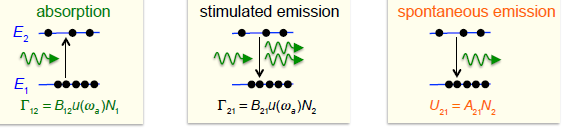
\includegraphics[scale=0.4]{img/image11.png}
			\captionof{figure}{Résolution circuit RC}
		\end{center}
		
		\subsection{Résolution rapide}
		\subsubsection{Avant l'échelon (condition initiale)}
		\begin{enumerate}
			\item Le courant est nul vu la loi à long terme
			\item La ddp est constante et supposée nulle (1)
			\item La ddp sur la résistance est nulle (2)
		\end{enumerate}
		\begin{equation}
		\left\{\begin{array}{l}
		i(t_0^-) = 0\\
		v_C(t_0^-) = 0\\
		v_R(t_0^-) = 0
		\end{array}\right.
		\end{equation}
		
		\subsubsection{En t$_0$ (court terme)}
		Que ce passe-t-il lorsque l'on applique l'échelon de tension $E$ ?
		\begin{enumerate}
			\item La ddp de la capa reste nulle (ne peut varier instantanément)
			\item En conséquence de (1), toute la tension se reporte sur $v_R$
			\item Le courant est donné par Ohm
		\end{enumerate}
		\begin{equation}
		\left\{\begin{array}{l}
		v_C(t_0^+) = v_C(t_0^-) = 0\\
		v_R(t_0^+) = E\\
		i(t_0^+) = E/R
		\end{array}\right.
		\end{equation}
		
		\subsubsection{En $t = \infty$ (long terme)}
		\begin{enumerate}
			\item Le courant est nul dans la capacité (loi long terme)
			\item En conséquence de (1) la ddp sur la résistance est nulle
			\item Toute la tension est reportée sur la capa : $v_C = E$.
		\end{enumerate}
		
		\subsection{Résolution rapide (2e exemple) : échelon des tension inverse}
		En partant de la situation finale du cas précédent, voyons ce qui se passe en appliquant une tension négative d'amplitude E. On suppose que l'instant $t=0$ représente le moment de retour à 0 de la tension $e(t)$.
		
		\subsubsection{Avant l'échelon (conditions initiales)}
		\begin{enumerate}
			\item Le curant et la ddp sur la résistance sont nuls
			\item La ddp sur la capa vaut E (capa chargée)
		\end{enumerate}
		
		\subsubsection{En $t_0$ (court terme)}
		Juste après l'échelon négatif $-E$
		\begin{enumerate}
			\item La source de tension prend la valeur nulle ! $e(t_0^+) = 0$
			\item La ddp de la capa ne peut pas varier directement : elle vaut encore $+E$
			\item En conséquence, la tension de la résistance vaut $-E$
			\item Le courant vaut donc $-E/R$
		\end{enumerate}
		
		\subsubsection{En $t = \infty$ (long terme)}
		\begin{enumerate}
			\item Le courant est nul dans la capacité (loi long terme)
			\item La tension est nulle dans la résistance à cause de (1)
			\item comme $v_R$ et $e(t)$ sont nulles, $v_C$ l'est aussi (capacité complètement déchargée)
		\end{enumerate}
		\begin{center}
			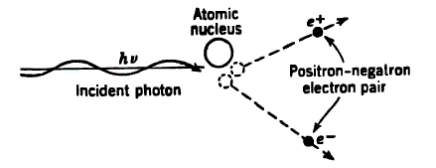
\includegraphics[scale=0.4]{img/image12.png}
			\captionof{figure}{Résolution circuit RLC en tension inverse}
		\end{center}
		
		\subsection{Constante de temps et fréquence de coupure (circuit du 1er ordre)}
		La durée de la charge et décharge de la capacité dépend de la constante de charge : $\tau = RC$.
		\begin{center}
			\begin{tabular}{|c|c|}
				\hline 
				Temps écoulé depuis l'échelon & Pourcentage de la (dé)charge réalisé \\ 
				\hline 
				$\tau$                           & 63                                      \\ 
				\hline 
				$3\tau$                          & 95                                      \\ 
				\hline 
				$5\tau$                          & 99                                      \\ 
				\hline 
			\end{tabular} 
		\end{center}
		On dira également que
		\begin{itemize}
			\item $v_C(t)$ est un filtre passe-bas de $e(t)$
			\item $v_R(t)$ est un filtre passe-haut de $e(t)$
		\end{itemize}
		La limite entre les fréquences hautes et basses est donnée par la fréquence de coupure définie par
		\begin{equation}
		f_0 = \frac{1}{2\pi\tau}
		\end{equation}
		\section{Analyse temporelle du circuit RL}
		\subsection{Résolution analytique complète}
		Si l'on attend suffisamment longtemps, par la loi \textit{long terme} $V = 0$ sur la self et $I = cste$ (pas forcément nul).\\
		On peut résoudre ce circuit analytiquement (syllabus page 212, slide 54- 57)
		
		\subsection{Résolution rapide}
		Même raisonnement que pour le circuit RC (page 212 pour le RL)
		
		\subsection{Constante de temps et fréquence de coupure}
		Les résultats ci-dessus nous apprennent que
		\begin{itemize}
			\item La tension $v_L(t)$ ne comporte que les hautes fréquences du signal $e(t)$ : filtre passe-haut
			\item La tension $v_R(t)$ ne comporte que les basses fréquences
		\end{itemize}
		
		\setcounter{section}{4}
		\section{Analyse temporelle du circuit RL (source sinusoïdale)}
		Au lieu d'avoir $e(t) = cste$, on a $e(t) = V_m\cos(\omega t + \alpha)$
		\begin{equation}
		Ri + L\frac{di}{dt} = e(t)
		\end{equation}
		Il suffit après de résoudre l'équation différentielle comme au cours d'Analyse I.
		
		\section{Circuit RLC avec précharge}
		La capacité à été préalablement chargée avec une tension $v_0$ et à l'instant $t=0$ on ferme l'interrupteur. L'équation du circuit est donc :
		\begin{equation}
		v_0 - \frac{1}{C}\int_{t_0}^t i(t)dt = L\frac{di}{dt} + Ri(t)
		\end{equation}
		
		\textsc{Ajouter les trois cas !!!}
		
		\chapter{Résoudre un circuit réactif dans le domaine fréquentiel}
		\section{Analyse fréquentielle : circuits linéaires en régime sinusoïdal}
		\subsection{Hypothèse et limitations de l'analyse fréquentielle}
		la sinusoïde est un signal \textit{monochromatique} : il n'a qu'une seule fréquence. C'est le signal le plus simple. Deux conditions sont a respecter :
		\begin{enumerate}
			\item Le circuit considéré est linéaire
			\item Toutes les sources sont purement sinusoïdale et de même fréquence
		\end{enumerate}
		Si ces hypothèses sont respectée, on parlera de \textbf{circuits linéaires en régime\footnote{Absence de transitoire} sinusoïdal}. Pour avoir une source purement monochromatique (obligatoire) il faut que le signal ne contienne pas de composante continue (sa moyenne doit être nulle) et que toutes les transitoires doivent avoir disparu.\\
		
		L'avantage est de résoudre le circuit sous forme paramétrique et d'avoir la réponse pour toutes les fréquences. Autre avantage, on sait de Fourier que tout signal sinusoïdal peut être décomposé en somme de sinusoïdes, ce qui nous permet d'utiliser le théorème de superposition.
		
		\subsubsection{Réponse d'un circuit linéaire et permanent en régime sinusoïdal}
		Le circuit est linéaire et permanent ssi $R, L$ et $C = cste$. La solution d'un tel systeme est $SGEH + SPEnH$ :
		\begin{equation}
		y(t) = \sum_{j=1}^n k_j e^{p_jt} + A\cos(\omega t + \alpha)
		\end{equation}
		
		\section{Caractérisation des fonctions périodiques}
		\subsection{Sinusoïde}
		La sinusoïde $a(t)$ est définie par ; sa valeur de crête (Â), sa pulsation $\omega$ et sa phase $\phi$ : $a(t) = \hat A\cos(\omega t + \phi)$
		
		\subsection{Fonction périodique quelconque}
		Toute fonction périodique peut s'écrire : 
		\begin{equation}
		f(t) = a_0 + \sum_{n=1}^\infty(a_n \cos(n\omega_0t) + b_n\sin(n\omega_0t) = A_0 + \sum_{n=1}^\infty A_n\cos(n\omega_0 t + \alpha_n)
		\end{equation}
		où $A_n = \sqrt{a^2_n + b^2_n}$ et $\tan(\alpha_n) = b_n/a_n$.
		
		\subsubsection{Valeur efficace}
		Il s'agit de la racine de la moyenne du carré (RMS = Root(Mean(Square()))) :
		\begin{equation}
		A_{eff} = \sqrt{\frac{1}{T}\int_0^T a^2(t) dt}
		\end{equation}
		Pour une sinusoïde (et pour une fonction périodique quelconque (slide 22)), on voit directement\footnote{$<\cos^2> = 1/2$} que $A_{eff} = \frac{A_m}{\sqrt{2}}$.
		
		\subsection{Puissance efficace}
		La valeur efficace est une valeur "moyenne" dissipant la même puissance que le signal.\\
		La puissance moyenne absorbée par une résistance au régime sinusoïdal est un facteur 1/52 :
		\begin{equation}
		P_R = \frac{1}{2}V_mI_m = V_{eff}I_{eff}
		\end{equation}
		\textbf{Attention !} $V_{crete}.I_{crete} = P_{max} \neq P_{moy}$
		\section{Phaseurs}
		\prop{Un phaseur est un nombre complexe représentant un signal sinusoïdal}\ \\
		Petit rappel de ce qui est vu au cours de \textit{Physique générale} slide 16.\\
		
		Le phaseur est un nombre complexe constant que l'on va rendre "tournant" en le multipliant par $e^{j\omega t}$.\\
		\textbf{Attention !} Le module du phaseur peut être défini en valeur efficace et non en valeur de crête, il faut faire attention à la convention utilisée! \\
		Deux erreurs fatales sont à éviter :
		\begin{enumerate}
			\item Le phaseur étant complexe, les opérations doivent aussi l'être : ne \textbf{pas} additionner uniquement les modules
			\item On n'utilise les phaseurs que s'il y a \textbf{une même fréquence} pour tous les signaux du circuit (pas de régime transitoire)
		\end{enumerate}
		\newpage
		\section{Impédances et admittances}
		\subsection{Impédance d'une inductance pure}
		\begin{wrapfigure}[10]{r}{3cm}
			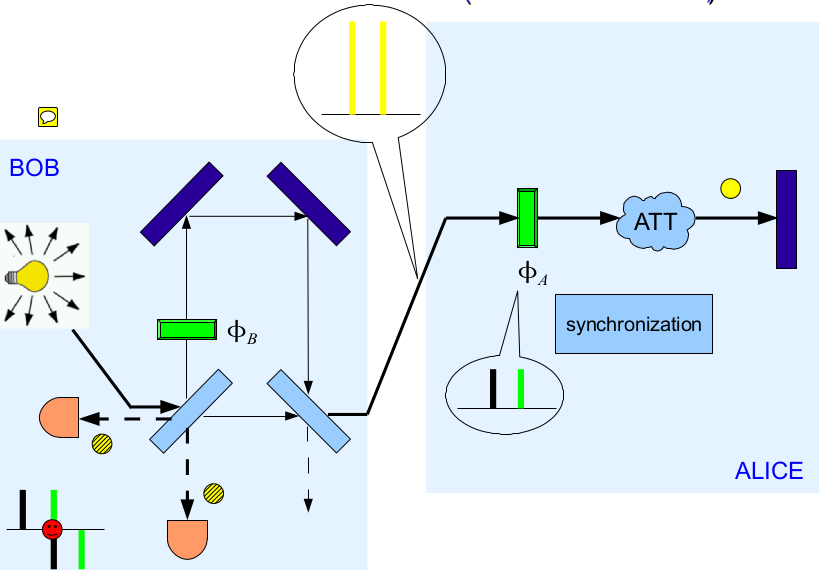
\includegraphics[scale=0.3]{img/image13.png}
			\captionof{figure}{Avance de $V$ sur $I$}
		\end{wrapfigure}
		Si l'on défini l'\textbf{impédance} d'une inductance $L$ comme le nombre complexe $Z_L = j\omega L$ on peut ré-écrire la loi fondamentale de l'inductance $v_l(t) = L\frac{di(t)}{dt}$ de la sorte : 
		\begin{equation}
		\phas{V} = Z\phas{I}
		\end{equation}
		
		\prop{Une impédance est un nombre complexe décrivant la relation entre la ddp et le courant agissant sur un dipôle (sous les hypothèses du régime sinusoïdal)}\ \\
		
		Par représentation dans le plan complexe, en prenant comme référence la phase de courant ($\theta = 0$) on peut se rendre compte que :\\
		
		\prop{Pour une inductance, la tension est \textit{en avance} de $\frac{\pi}{2}$ sur le courant.}\ \\
		
		En analysant le domaine fréquentiel, on se rend compte que l'impédance tend vers 0 pour les basses fréquences mais est très élevée pour les hautes fréquences :\\
		
		\prop{L'impédance d'une inductance est proportionnelle à $\omega$.\\
			Son module est donc faible en b.f. et élevé en h.f.}
		
		\subsection{Impédance d'une capacité pure}
		\begin{wrapfigure}[7]{l}{3cm}
			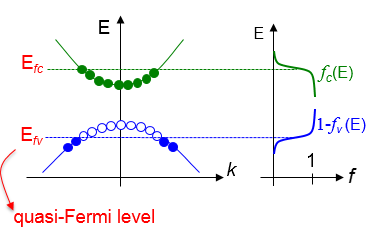
\includegraphics[scale=0.3]{img/image14.png}
			\captionof{figure}{Retard de $V$ sur $I$}
		\end{wrapfigure}
		Même constat que pour l'inductance, si ce n'es que l'impédance d'une capacité $C$ permettant d'écrire $\phas{V} = Z_C\phas{I}$ est\footnote{Comme pour $X_L$ il y a une loooongue démo dans le sylla (p. 241) mais je ne sais pas s'il faut l'étudier.} : 
		\begin{equation}
		Z_C = \frac{1}{j\omega C}
		\end{equation}
		En analysant le domaine fréquentiel, on se rend cette fois compte que :\\
		\prop{Pour une capacité, la tension est \textit{en retard} de $\frac{\pi}{2}$ sur le courant.}\ \\
		
		En analysant l'impédance, on remarque que celle-ci est bien cohérente avec le fait que celle-ci s'oppose à une variation brusque de la ddp à ses bornes (injecter du $I$ est plus simple avec une impédance faible):\\
		
		\prop{L'impédance d'une capacité est inversement proportionnelle à $\omega$.\\
			Son module est donc élevé en b.f. et faible en h.f.}
		
		\subsection{Impédance d'une résistance pure}
		Ca va vite, on peut directement écrire :
		\begin{equation}
		\phas{V} = R\phas{I}
		\end{equation}
		La résistance pure n'introduit donc aucun déphasage au contraire de l'inductance.
		
		\subsection{Impédance d'un dipôle quelconque}
		Pour faire simple, l'impédance est le rapport d'un phaseur de tension sur un phaseur de courant. Les résultats obtenus  précédemment peuvent être généralisé :\\
		
		\prop{L'impédance est une généralisation de la notion de résistance à un nombre complexe quelconque, permettant ainsi, sous les hypothèses du régime sinusoïdal, dé décrire le déphasage intervenant entre signant de tension et de courant.}\ \\
		
		Elle permet ainsi de généraliser la loi d'Ohm aux signaux déphasés, mais aussi d'utiliser les lois de mise en parallèle et série, la procédure canonique de résolution de circuit, le théorème de superposition et l'impédance d'entrée et de sortie d'un équivalent de Thévenin.
		
		\subsection{Admittance, conductance et suceptance}
		L'admittance traduit la relation entre $\phas{I}$ et $\phas{V}$ :
		\begin{equation}
		Y(j\omega) = \frac{\phas{I}}{\phas{V}}
		\end{equation}
		L'admittance est l'inverse de l'impédance $Y = \frac{1}{Z}$ \textbf{mais} on ne peut pas écrire pour un dipôle quelconque que la conductance est l'inverse de la résistance !
		
		\subsubsection{Loi de Kirchhoff ? Loi des mailles ?}
		Elles restent toutes deux valables à condition de les écrire en \textbf{complexes} ! Par exemple, pour la loi des mailels :
		\begin{equation}
		\phas{V_1} + \phas{V_2} + \phas{V_3} = 0
		\end{equation}
		Attention à l'addition complexe (2 composantes) !
		
		\subsubsection{Association d'impédances}
		Deux dipôle sont équivalent (au sens de Thévenin) s'ils sont caractérisé par la même relation entre $i(t)$ et $v(t)$ (ou même $Z$ en régime sinusoïdal) := même comportement externe.\\
		Revoir \textbf{réseau en échelle}, slide 46.
		
		\section{Expressions de la puissance en formalisme fréquentiel}
		\subsection{/2/3 - Puissance instantanée, puissance active et réactive}
		\begin{wrapfigure}[7]{l}{4.7cm}
			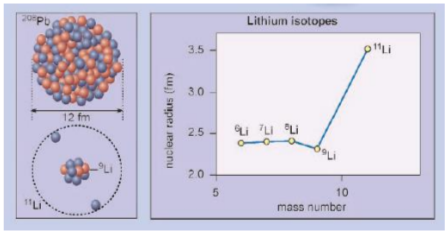
\includegraphics[scale=0.3]{img/image15.png}
			\captionof{figure}{Puissance active}
		\end{wrapfigure}
		La \textit{puissance instantanée} est la puissance à fournir/absorber par un dipôle à l'instant $t$\footnote{Convention récepteur} :
		\begin{equation}
		p(t) = i(t)v(t)
		\end{equation}
		La \textit{puissance active} (P) est la moyenne de la puissance instantanée, expression indépendante du temps (c'est une \textbf{constante}) :
		\begin{equation}
		P = \frac{1}{T}\int_{t_0}^{t_0+T} p(t) dt
		\end{equation}
		Dans le cas du régime sinusoïdal : $v(t) = V\cos(\omega t + \alpha), i(t) = \hat A\cos(\omega t + \beta)$. La puissance instantanée vaut le produit des deux, ce qui peut également s'écrire :
		\begin{equation}
		p(t) = \underbrace{\frac{V\hat I}{2}\cos(\alpha - \beta)}_{\text{Puissance active}} + \frac{v\hat I}{2}\cos(2\omega t + \alpha + \beta)
		\end{equation}
		Le premier terme étant constant, il s'agit de la puissance active. La puissance instantanée comprend donc la puissance active et une composante sinusoïdale de $2f$.\\
		La puissance active dépend donc des amplitudes de $V$ et $I$ et du consinus de leur déphasage.\\
		
		On peut ré-écrire la puissance instantanée : 
		
		
		
		
		
		\begin{equation}
		p(t) = A[1 + \cos(2\omega t + 2\alpha)] + Q \sin(2\omega t + 2\alpha)\ \ \ \text{où}\ \left\{\begin{array}{l}
		Q = \frac{1}{2}V_mI_m\sin\phi\\
		P = \frac{1}{2}V_mI_m\cos\phi
		\end{array}\right.
		\end{equation}
		La premier terme correspond à la puissance absorbée par la charge (>0) d'amplitude $P$ = puissance active.\\
		Le deuxième terme est la puissance périodiquement échangée entre la source et la charge d'amplitude $Q$ = puissance réactive\footnote{S'exprime en VAR : volt-ampère réactif.}.
		\begin{center}
			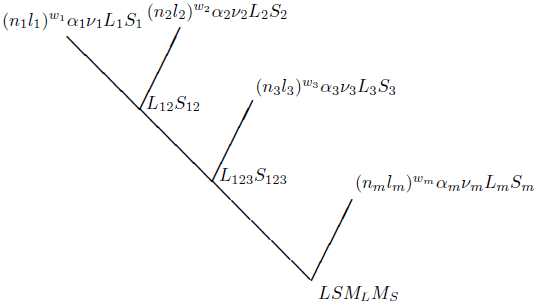
\includegraphics[scale=0.6]{img/image16.png}
			\captionof{figure}{Puissance active/réactive}
		\end{center}
		
		\setcounter{subsection}{3}
		\subsection{Expressions de $P$ et $Q$ pour les trois charges élémentaires}
		\subsubsection{Résistance}
		Pour une résistance $R$, la puissance instantanée est donnée par $p(t) = Ri^2(t)$ : elle est toujours positive ou nulle : élément dissipatif (chaleur).
		En régime sinusoïdal $\phi = 0 \Rightarrow  \left\{\begin{array}{l}
		Q = V_mI_m\sin\phi = 0\\
		P = V_mI_m\cos\phi = V_mI_m
		\end{array}\right.$\\
		On retrouve que $P = \frac{V_{eff}^2}{R}$ et que la puissance instantanée se réduit à :
		\begin{equation}
		p(t) = P[1 + \cos(2\omega t + 2\alpha)]
		\end{equation}
		
		\subsubsection{Inductance}
		Ici, contrairement à la résistance, l'inductance peut restituer de l'énergie : c'est un élément non dissipatif. En régime sinusoïdal, nous avons pour l'inductance :
		\begin{eqnarray}
		v(t) &=& \omega L\hat I\cos(\omega t + \beta + \frac{\pi}{2})\\
		i(t) &=& Î\cos(\omega t + \beta)
		\end{eqnarray}
		Comme le courant et la tension sont déphasé de $\phi = \frac{\pi}{2}$ on retrouve : $\Rightarrow  \left\{\begin{array}{l}
		Q = V_mI_m\sin\phi = +V_{eff}I_{eff}\\
		P = V_mI_m\cos\phi = 0
		\end{array}\right.$\\
		On retrouve que $Q = \frac{1}{2}\omega LI_{eff}^2$ et la puissance instantanée se réduit à : 
		\begin{equation}
		p(t) = -Q\sin(2\omega t + 2\beta)
		\end{equation}
		
		\subsubsection{Capacité}
		En régime sinusoïdal, nous avons pour la capacité :
		\begin{eqnarray}
		v(t) &=& V\cos(\omega t + \alpha)\\
		i(t) &=& \omega CV\cos(\omega t + \alpha + \frac{\pi}{2})
		\end{eqnarray}
		La tension et le courant sont déphasé de $\phi = -\frac{\pi}{2}$, on a donc :
		\begin{eqnarray}
		P &=& V_{eff}I_{eff}\cos\phi = 0\\
		Q &=& V_{eff}\sin_{eff}\sin\phi = -V_{eff}I_{eff}
		\end{eqnarray}
		On retrouve que $Q = -\omega CV^2$ et la puissance instantanée se réduit à : 
		\begin{equation}
		p(t) = Q\sin(2\omega t + 2 \alpha)
		\end{equation}
		
		\subsection{Interprétation du facteur de puissance}
		\begin{wrapfigure}[12]{l}{4.7cm}
			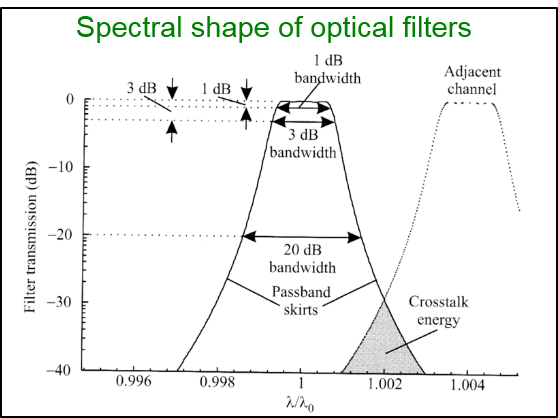
\includegraphics[scale=0.5]{img/image17.png}
			\captionof{figure}{$\cos\phi$}
		\end{wrapfigure}
		Le facteur de puissance d'une charge est le cosinus du déphasage entre $V$ et $I$. Pour la puissance active dans un dipôle :
		\begin{equation}
		P = V_{eff}I_{eff}.\underbrace{\cos\phi}_{\text{Facteur de puissance}}
		\end{equation}
		Le $\cos\phi$ d'une impédance $Z$ (signaux déphasés) traduit la réduction de la puissance dissipée par rapport à une résistance (signaux en phase).\\
		
		Un dipôle est passif si l'énergie absorbée depuis l'origine est à tout instant positif ou  nulle. En régime sinusoïdal il en résulte :
		\begin{itemize}
			\item $P \geq 0$
			\item Ou encore : $Re[Z(j\omega)] \geq 0$
			\item Ou encore : $-\frac{\pi}{2} \leq \phi \leq \frac{\pi}{2}$
		\end{itemize}
		
		\setcounter{subsection}{6}
		\subsection{Puissance et superposition}
		Peut-on sommes les puissances pour un signal composé de plusieurs harmoniques (= sinusoïde) ? 
		\begin{itemize}
			\item La \textit{puissance instantanée} totale n'est \textbf{pas} la somme des puissances instantanées de chaque harmonique
			\item La \textit{puissance active} totale \textbf{est} la somme des puissance active de chaque harmonique
		\end{itemize}
		Démo dans le syllabus page 258.
		
		
		\part{Théorie des champs}
		\setcounter{chapter}{0}
		\chapter{Introduction à la théorie des champs}
		\section{Les équations de Maxwell}
		\subsection{A quoi servent les équations de Maxwell ?}
		Elles servent à \textit{prévoir et expliquer les forces d'origine électromagnétique dans des configurations non élémentaires de charges et/ou de courants.}
		
		\subsection{Le principe : les forces sont dues aux champs, qui eux-mêmes sont dus aux sources}
		Le principe des équations de Maxwell est le suivant : $source\ \rightarrow\ champ\ \rightarrow force$ principe bien illustré par la force de Lorentz : $\vec{F} = q(\vec{E} + \vec{v}\times\vec{B})$ ou la source $q$ génère les champs qui eux-mêmes génèrent une force.\\
		\prop{Une charge n'exerce pas de force sur elle-même : elle n'interagit pas avec le champ qu'elle provoque, mais uniquement avec le champ dû aux \textit{autres} charges.}
		
		\section{Qu'est ce qu'un champ ?}
		Tout d'abord, un \textbf{champ} est \textit{une grandeur définie partout dans l'espace}.\\
		Il existe des champs scalaire (possède une valeur en chaque point de l'espace, comme $V$) et des vectoriels (lorsque chaque point est à plus de 1D, comme $\vec{B}$).\\
		Tout champ vectoriel peut-être décomposé en une composante lamellaire (irrotationelle) et solénoïdale (rotationelle). Ce sera détaillé plus bas, pas d'impatience ! 
		\begin{equation}
		\vec{a} = \vec{a}_{div} + \vec{a}_{rot}
		\end{equation}
		
		\section{Les outils de l'analyse vectorielle}
		\subsection{Le flux}
		Le \textbf{flux} d'un vecteur\footnote{Il s'agit d'une grandeur scalaire, ce n'est pas un champ.} est l'intégrale sur une certaine surface $S$, du produit scalaire de ce vecteur par l'élément de surface:
		\begin{equation}
		\Phi = \iint_S \vec{a}.d\vec{S}
		\end{equation}
		Cette expression n'est \textbf{pas} la même que la suivante, qui concerne les surfaces fermées :
		\begin{equation}
		\Phi = \oiint_S \vec{a}.d\vec{S}
		\end{equation}
		
		
		\subsection{Circulation}
		La \textbf{circulation} d'un vecteur est l'intégrale, sur un certain trajet $L$, du produit scalaire de ce vecteur par l'élément de longueur :
		\begin{equation}
		\xi = \int_L \vec{a}.d\vec{l}
		\end{equation}
		
		\subsection{Divergence}
		La \textbf{divergence}\footnote{La divergence est un champ scalaire} d'un vecteur est définie comme la somme des dérivées spatiales des composantes de ce vecteurs, selon leurs axes respectifs :
		\begin{equation}
		div(\vec{a}) = \frac{\partial a_x}{dx} + \frac{\partial a_y}{dy} + \frac{\partial a_z}{dz}
		\end{equation}
		
		\subsubsection{Interprétation}
		La divergence traduit la \textit{disposition spatiale} de ce vecteur.\\
		La divergence d'un vecteur en un point $P$ n'est non-nulle que si ce champ varie dans l'espace autour de $P$.
		\begin{itemize}
			\item $div > 0$ : "génération" de champ à cen endroit : source.
			\item $div < 0$ : "absorption" de champ à cet endroit : puits.
		\end{itemize}
		Un théorème important est celui d'\textit{Ostrogradsky} :
		\begin{equation}
		\oiint_S \vec{a}.d\vec{S} = \iiint_\tau div(\vec{a}).dV
		\end{equation}
		ou en français : le flux d'un vecteur sur une surface fermée est égal à l'intégrale de volume de la divergence de ce vecteur sur le volume compris dans cette surface fermée.
		
		\subsection{Rotationnel}
		Le \textbf{rotationnel}\footnote{Le rotationnel est un champ vectoriel} d'un vecteur $\vec{a}$ est défini comme :
		\begin{equation}
		rot(\vec{a}) = \vec{\nabla} \times \vec{a}
		\end{equation}
		Le théorème magique est cette fois-ci celui de \textit{Stokes}\footnote{L'orientation relative du contour et de la normale à la surface est déterminée par la règle de la main droite} : 
		\begin{equation}
		\oint_C \vec{a}.d\vec{l} = \iint_S rot(\vec{a}).d\vec{S}
		\end{equation}
		Cet "outil" traduit également la disposition spatiale d'un vecteur : $rot(\vec{a})$ est un vecteur dont :
		\begin{itemize}
			\item La direction est normale au plan pour lequel la circulation du vecteur (le long d'un parcours fermé élémentaire centré sur le point $P$) est maximum.
			\item Le module vaut la valeur de cette circulation maximale, par unité de surface.
		\end{itemize}
		En résumé, \textit{le rotationnel de $\vec{a}$ en $P$ est un vecteur qui donne l'axe (et l'intensité) de rotation du champ $\vec{a}$ sur lui-même, immédiatement autour du point $P$.}
		
		
		
		\section{Que signifient les équations de Maxwell ?}
		\subsection{De quoi parlent les équations de Maxwell ?}
		Sous leur forme intégrales, ces équations sont :
		\begin{equation}
		\left\{\begin{array}{l}
		\oint_S \vec{E}.d\vec{S} = \dfrac{Q}{\epsilon_0}\\
		\oint_C \vec{E}.d\vec{l} = -\dfrac{d}{dt}\int_S \vec{B}.d\vec{S}\\
		\oint_S \vec{B}.d\vec{S} = 0\\
		\oint_C \vec{B}.\vec{dl} = \mu_0 I + \epsilon_0\mu_0\dfrac{d}{dt}\int_S \vec{E}.d\vec{S}
		\end{array}\right.
		\end{equation}
		
		\subsection{Loi de Gauss}
		\begin{equation}
		\oint_S \vec{E}.d\vec{S} = \frac{Q}{\epsilon_0}\ \ \ \ \underbrace{\Leftrightarrow}_{Ostrogradsky}\ \ \ \ div\ \vec{E} = \frac{\rho}{\epsilon_0}
		\end{equation}
		Au niveau de la disposition spatiale, $\vec{E}$ a une \textit{composante lamellaire} : il existe des sources de "flux" électriques : $Q$.\footnote{$Q$ "provoque" $\vec{E}_{div}$}\\
		\prop{$\vec{E}$ converge ou diverge aux points où se trouvent des charges électriques}
		
		\subsection{Loi de Fadaday}
		\begin{equation}
		\oint_C \vec{E}.d\vec{l} = -\dfrac{d}{dt}\int_S \vec{B}.d\vec{S}\ \ \ \ \underbrace{\Leftrightarrow}_{Stokes}\ \ \ \ rot\ \vec{E} = - \dfrac{\partial \vec{B}}{\partial t}
		\end{equation}
		Caractérise la composante \textit{solénoïdale} de $\vec{E}$. A certains endroits, le champ $\vec{E}$ va tourner sur lui même lorsque $\vec{B}$ varie (la source de cette composante solénoïdale est la dérivée temporelle de $B$).\\
		\prop{$\vec{E}$ forme des "boucles" autour des directions où le flux de $\vec{B}$ varie dans le temps}
		
		\subsection{Absence de monopôle magnétique}
		\begin{equation}
		\oint_S \vec{B}.d\vec{S}\ \ \ \ \underbrace{\Leftrightarrow}_{Ostrogradsky}\ \ \ \ div\ \vec{B} = 0
		\end{equation}
		Cela caractérise la composante lamellaire de $\vec{B}$ : indique que $\vec{B}$ ne possède pas de disposition convergente/divergente, les lignes de champs ne se croisent jamais. \\
		\prop{$\vec{B}$ ne converge ou ne diverge en aucun point. Il n'existe pas de "charges magnétiques".}
		
		
		\subsection{Loi d'Ampère}
		\begin{equation}
		\oint_C \vec{B}.\vec{dl} = \mu_0 I + \epsilon_0\mu_0\dfrac{d}{dt}\int_S \vec{E}.d\vec{S}\ \ \ \ \underbrace{\Leftrightarrow}_{Stokes}\ \ \ \ rot\ \vec{B} = \mu_0\vec{J} + \epsilon_0\mu_0 \dfrac{\partial \vec{E}}{\partial t}
		\end{equation}
		Caractérise la composante solénoïdale de $\vec{B}$ : $\vec{B}$ possède une telle disposition à certains endroits.\\
		Il existe deux sources différentes à cette composante : le courant électrique et la dérivée temporelle de $\vec{E}$\footnote{A un facteur près}.\\
		\prop{$\vec{B}$ forme des "boucles" autour des courants et autour des directions où le flux de $\vec{E}$ varie dans le temps.}
		
		
		\section{Équation de continuité (conservation de la charge)}
		Si la charge diminue au sein d'une surface, c'est qu'un courant positif est sorti de celle-ci\footnote{Démonstration page 24-25}.
		\begin{equation}
		\oint_S \vec{J}.d\vec{S} = - \dfrac{dQ}{dt}\ \ \ \ \underbrace{\Leftrightarrow}_{Ostrogradsky}\ \ \ \ div\ \vec{J} = -\frac{d\rho}{dt}
		\end{equation}
		
		\subsubsection{Cas stationnaire}
		En statiques, cette équation de continuité vaut 0. Cela signifie que $\vec{J}$ est purement rotationnel.
		
		
		
		
		
		
		
		
		
		\chapter{Électrostatique dans le vide}
		\section{Équations de l'électrostatique}
		\subsubsection{Découplage des équations de Maxwell}
		Comme $\rho$ et $\vec J$ sont stationnaires, les équations de Maxwell peuvent se découpler en deux paires d'équations indépendantes (gauche = électrostatique, droite = magnétostatique) : 
		\begin{equation}
		\left\{\begin{array}{l}
		\oint_S \vec{E}.d\vec{S} = \frac{Q}{\epsilon_0}\\
		\oint_C \vec{E}.d\vec{l} = 0
		\end{array}\right. \ \ \\ \ \ \ \ \ \ \ \left\{\begin{array}{l}
		\oint_S \vec{B}.d\vec{S} = 0\\
		\oint_C \vec{B}.d\vec{l} = \mu_0 I
		\end{array}\right.
		\end{equation}
		
		\section{Champ électrique}
		\subsection{Champ électrique dû à une charge ponctuelle}
		La démonstration s'obtient par $\vec{F} = q\vec{E}$ et le théorème de Gauss pour trouver $\vec{E}$ (\textit{cf. page 29 - 30})
		\begin{equation}
		\vec{E}(P) = \frac{q}{4\pi\epsilon_0r^2}\vec{1_r}
		\end{equation}
		Résultat facilement généralisable à plusieurs charges ou pour des répartitions de charges.
		
		
		\section{Potentiel électrique}
		Le gradient d'un \textbf{scalaire} est un vecteur : 
		\begin{equation}
		grad\ u = \frac{\partial u}{\partial x}\vec{1_x} + \frac{\partial u}{\partial y}\vec{1_y} + \frac{\partial u}{\partial z}\vec{1_z}
		\end{equation}
		Il s'agit d'une généralisation de la dérivée à des fonctions à trois variables. Il indique la direction de croissance maximum d'une fonction scalaire\footnote{$du = grad(u).\vec{dl}$}.\\
		La différence des valeurs de $u$ entre deux points $A$ et $B$ vaut la \textit{circulation} du gradient de $u$ :
		\begin{equation}
		u(B) - u(A) = \int_A^B du = \int_A^B grad(u).\vec{dl}
		\end{equation}
		En présence d'un champ lamellaire (conservatif) la circulation du champ ne dépend pas du trajet suivi. On peut donc définir une grandeur scalaire $U$, appelée "potentiel" telle que :
		\begin{equation}
		\int_A^B \vec{a}.\vec{dl} = W_{AB} = U(B) - U(A) = \int_A^B grad(U).\vec{dl}
		\end{equation}
		Comme en électrostatique $\vec{E}$ est lamellaire on peut définir une grandeur $V$ telle que :
		\begin{equation}
		\vec{E} = - grad(V)
		\end{equation}
		Ajouter une constante à $V$ ne changera rien : on ne peut donc pas connaître la valeur de $V$ qui n'est définie qu'à une constante près : justifie en théorie des circuits le choix arbitraire de la masse.
		\begin{wrapfigure}[7]{r}{4.7cm}
			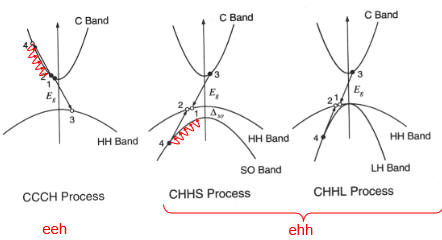
\includegraphics[scale=0.3]{img/image31.png}
			\captionof{figure}{Signe négatif}
		\end{wrapfigure}
		\subsubsection{Pourquoi un signe négatif ?}
		\begin{itemize}
			\item Comme les charges sont sources, $\vec{E}$ diverge à partir ce celles-ci
			\item Une charge positive dans $\vec{E}$ subit une force qui l'\textit{écarte} des charge positive.
			\item Si pas de -, le potentiel serait plus élevée au charges négatives que positives.
		\end{itemize}
		Cela correspond donc au fait que le potentiel va être orienté du potentiel le plus faible vers le plus élevé (tête de la flèche - bas de la flèche).\\
		
		Les équation de Poisson et Laplace sont à connaître (page 34) ainsi que la démonstration, slide 73.
		
		
		
		\setcounter{section}{4}
		\section{Énergie électrostatique}
		\subsection{Énergie électrostatique d'une charge}
		L'énergie électrostatique d'une charge ponctuelle $q$ vaut :
		\begin{equation}
		W_e = qV
		\end{equation}
		\begin{proof}\ \\
			Le signe négatif de la force vient du fait qu'il faut s'opposer à la force s'exerçant sur la charge test. Si $A$ est pris à l'infini, son potentiel y est nul.
			\begin{eqnarray}
			W_{AB} &=& \int_A^B \vec{F}_{ext}.d\vec{l}\\
			W_{AB} &=& -\int_a^B q\vec{E}.d\vec{l}\\
			W_{AB} &=& +q(V(B) - V(A))\\
			W_{AB} &=& qV(B)
			\end{eqnarray}
		\end{proof}
		
		\subsection{Énergie d'un ensemble de charge}
		En généralisant pour $n$ charges :
		\begin{equation}
		W = \frac{1}{4\pi\epsilon_0}\sum_{i = 1}^{n}\sum_{j=1, j>i}^n \frac{q_iq_j}{r_{ij}}
		\end{equation}
		La démonstration est donnée page 38.
		
		\subsection{Énergie électrostatique d'une distribution de charge}
		\begin{equation}
		w_e = \frac{1}{2}\int_\tau \rho V d\tau
		\end{equation}
		
		\subsection{Densité d'énergie électrostatique}
		La démonstration se trouve à la page 39 (pas connaître).
		\begin{equation}
		w_e = \frac{1}{2}\epsilon_0E^2
		\end{equation}
		
		
		\section{Conditions aux limites de part et d'autre d'une surface chargée}
		\subsection{Variation du champ $\vec{E}$}
		\begin{wrapfigure}[14]{r}{3cm}
			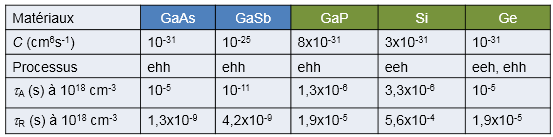
\includegraphics[scale=0.5]{img/image32.png}
			\captionof{figure}{Champ d'une surface chargée}
		\end{wrapfigure}
		Le champ électrique est noté $\vec{E_1}$ et $\vec{E_2}$ au voisinage immédiat de la surface et peut être décomposé en une composante tangentielle et une composante normale à la surface :
		\begin{equation}
		\left\{\begin{array}{l}
		\vec{E_1} = \vec{E_{1t}} + \vec{E_{1n}}\\
		\vec{E_2} = \vec{E_{2t}} + \vec{E_{2n}}
		\end{array}\right.
		\end{equation}
		On peut montrer que le champ électrique n'est pas identique de part et d'autre de la surface et qu'il subit une discontinuité :
		\begin{equation}
		\vec{E_1} - \vec{E_2} = \frac{\sigma}{\epsilon_0}\vec{1_n}
		\end{equation}
		\begin{proof}\ \\
			\textbf{Composante normale}\\
			On sait par Gauss :
			\begin{equation}
			\oint_{cyl} \vec{E}.d\vec{S} = \frac{Q}{\epsilon_0} = \frac{\sigma S_b}{\epsilon_0}
			\end{equation}
			En faisant tendre la surface latérale du cylindre vers zéro pour considérer $\vec{E}$ constant : 
			\begin{equation}
			\vec{E}_1.\vec{1_n}S - \vec{E_2}.\vec{1_n}S = (E_{1n} - E_{2n})S = \frac{\sigma S}{\epsilon_0}
			\end{equation}
			On a donc :
			\begin{equation}
			E_{1n} - E_{2n} = \frac{\sigma }{\epsilon_0}
			\end{equation}
			Ce qui peut aussi s'écrire :
			\begin{equation}
			||\vec{E}||.\vec{1_n} = \frac{\sigma}{\epsilon_0}
			\end{equation}\ \\
			\textit{La composante normale du champ subit une discontinuité proportionnelle à la densité surfacique de charge.}\ \\
			
			\textbf{Composante tangentielle}\\
			
			Considérons pour la composante tangentielle (selon $x$ par exemple), un contour rectangulaire à cheval sur la surface chargée de hauteur infinitésimale. Maxwell nous donne :
			\begin{equation}
			\oint_C \vec{E}.\vec{dl} =0
			\end{equation}
			Mais encore :
			\begin{equation}
			\int_a^b (\vec{E_1} - \vec{E_2}).\vec{dl} = 0
			\end{equation}
			On a donc :
			\begin{equation}
			\vec{E_{1t}} = \vec{E_{2t}}
			\end{equation}
			Ce qui peut aussi s'écrire :
			\begin{equation}
			||\vec{E}||\times \vec{1_N} = \vec{0}
			\end{equation}
			Et l'on retrouve bien le résultat annoncé.\\
			\textit{Au passage d'une surface chargée, le composante tangentielle $\vec{E_t}$ est continue.}
			
			
		\end{proof}
		
		\subsection{Variation du potentiel au travers d'une surface chargée}
		On peut déduire le potentiel via le champ. En effet :
		\begin{equation}
		V_1 - V_2 = - \int_a^b \vec{E}.d\vec{l}
		\end{equation}
		En prenant un chemin d'intégration (non fermé) entre $a$ et $b$ de la sorte qu'ils tendent vers zéro, le membre de droite devient nul ($l = 0$). On a donc :
		\begin{equation}
		V_1 = V_2
		\end{equation}
		\textit{AU passage d'une surface chargée, le potentiel électrique $V$ est continu}\\
		
		Par contre le gradient n'est pas continu ! En effet :
		\begin{equation}
		-grad(V)_1 + grad(V)_2 = \frac{\sigma}{\epsilon_0}\vec{1_n}
		\end{equation}
		Ou encore :
		\begin{equation}
		\left(\frac{\partial V}{\partial n}\right)_1 - \left(\frac{\partial V}{\partial n}\right)_2 = -\frac{\sigma}{\epsilon_0}
		\end{equation}
		En notant la dérivée normale\footnote{Taux de variation dans la direction normale à la surface} du potentiel :
		\begin{equation}
		\left(\frac{\partial V}{\partial n}\right) = grad(V).\vec{1_n}
		\end{equation}
		\textit{Au passage d'une surface chargée, la dérivée normale du potentiel subit une discontinuité proportionnelle à la densité surfacique de charge.}
		
		\subsection{Cas du conducteur parfait}
		Si le champ électrique est nul d'un côté de la surface ($\vec{E_2} = \vec{0}$) les conditions aux limites se réduisent à  : 
		\begin{equation}
		\left\{\begin{array}{l}
		\vec{E_1} = \frac{\sigma}{\epsilon_0}\vec{1_n}\\
		\left(\frac{\partial V}{\partial n}\right)_1 = -\frac{\sigma}{\epsilon_0}
		\end{array}\right.
		\end{equation}
		
		
		\section{Condensateur et coefficient de capacité}
		\subsection{Conducteurs formant un condensateur}
		\begin{wrapfigure}[12]{r}{4cm}
			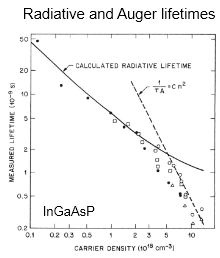
\includegraphics[scale=0.5]{img/image33.png}
			\captionof{figure}{Condensateur}
		\end{wrapfigure}
		Soit deux conducteur portant des charges opposées. Lors de l'équilibre électrostatique :
		\begin{itemize}
			\item Le champ électrique est nul à l'intérieur de chaque conducteur.
			\item Tous les points à l'intérieur et sur la surface d'un conducteur sont au même potentiel.
			\item Toute la charges e répartir à la surface des conducteurs sous forme d'une densité superficielle $\sigma$.
			\item Le champ électrique à l'extérieur, et au voisinage immédiat du conducteur, est normal à la surface de celui-ci :
			\begin{equation}
			\vec{E} = \frac{\sigma}{\epsilon_0}\vec{1_n}
			\end{equation}
		\end{itemize}
		\subsection{Coefficient de capacité}
		Comme $V \propto \vec{E}$ et $\vec{E} \propto Q$, on peut dire que $V \propto Q$. En notant $C$ le coefficient de proportionnalité, on peut écrire : 
		\begin{equation}
		Q = CV
		\end{equation}
		Elle a pour unité le \textbf{farad}. C'est un facteur purement géométrique (forme des armatures). Un tel système de deux conducteurs est un \textit{condensateur}.
		
		
		\subsection{Condensateur plan}
		Un grand classique du cours de \textit{Physique Générale}. En supposant que la distance entre les plaques est bien plus petite que la dimension des armatures et que $\vec{E}$ est normal à celles-ci :
		\begin{equation}
		E = \frac{Q}{\epsilon_0A}
		\end{equation}
		Comme $V = Ed$, on trouve que $V = \frac{Qd}{\epsilon_0 A}$ et la capacité de ce condensateur plan vaut :
		\begin{equation}
		C = \frac{\epsilon_0A}{d}
		\end{equation}
		
		\subsection{Énergie accumulée dans un condensateur}
		Le travail nécessaire pour séparer les charge et les transférer d'une armature à l'autre via le circuit \textit{extérieur} du condensateur est donné par :
		\begin{equation}
		W = \frac{1}{2}CV^2
		\end{equation}
		Trois démonstrations sont présentée dans le cours (page 49-50) et dans les slides (97-99) mais c'est bien connu depuis l'année passée!
		
		\section{Forces électrostatiques}
		\subsection{Forces entre armatures dans un condensateur plan}
		Quel travail faut-il effectuer pour déplacer les armatures de $\delta d$ : $\delta W = F_{ext}\delta d$. Par conservation d'énergie, $W$ doit valoir l'expression trouvée ci-dessus. La variation de travail vaut dès lors :
		\begin{equation}
		\delta W = \delta\left(\dfrac{Q^2}{2C}\right)
		\end{equation}
		Deux cas sont à considérer.
		
		\subsubsection{Cas 1 : condensateur à charge constante}
		Si le condensateur est déconnecté de la pile, $Q$ reste constante et on peut le sortir de la variation :
		\begin{equation}
		\delta W = \frac{Q^2}{2}\delta\left(\frac{1}{C}\right)
		\end{equation}
		Connaissant l'expression de $C$ on trouve :
		\begin{equation}
		\delta\left(\frac{1}{C}\right) = \frac{\delta d}{\epsilon_0A}
		\end{equation}
		Finalement :
		\begin{equation}
		F_{ext} = \frac{\delta W}{\delta d} = \frac{Q^2}{2\epsilon_0A}
		\end{equation}
		Quantité forcément positive : existe une force électrique d'attraction entre les armatures qui tend à augmenter la capacité. La mesure de cette force permet de mesurer $Q$ : principe d'un électromètre.
		
		\subsubsection{Cas 2 : Condensateur à ddp constante}
		Si le condensateur reste connecté à la pile durant le déplacement virtuel la ddp sera constante et c'est $Q$ qui variera : $\delta Q = V \delta C$. La source doit fournir un travail pour donner cette charge:
		\begin{equation}
		\delta W_{source} = V\delta Q = V^2\delta C
		\end{equation}
		Comme on connait l'expression de $W$ :
		\begin{equation}
		\delta\left(\frac{1}{2}CV^2\right) = \frac{1}{2}V^2\delta C
		\end{equation}
		Par conservation : travail de la source + travail mécanique = variation d'énergie potentielle :
		\begin{equation}
		V^2\delta C + F_{ext}\delta d = \frac{1}{2}V^2\delta C
		\end{equation}
		On trouve que $F_{ext}\delta d = -\frac{1}{2}V^2\Delta C$. Comme $\delta C = -\frac{\epsilon A}{d^2}\delta d$ on trouve la force entre les armatures :
		\begin{equation}
		F_{ext} = \frac{\epsilon_0 A}{2d^2}V^2
		\end{equation}
		La mesure de cette force permet d'obtenir la ddp : principe du voltmètre électrostatique.
		
		\subsection{Forces s'exerçant sur une charge de surface et pression électrostatique}
		\subsubsection{Champ électrique au sein d'une surface chargée (démo pas à connaître)}
		\begin{wrapfigure}[12]{l}{5.3cm}
			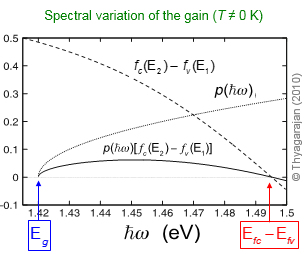
\includegraphics[scale=0.5]{img/image34.png}
			\captionof{figure}{Calcul de la pression électrostatique}
		\end{wrapfigure}
		Considérons un "patch" infinitésimal sur la surface. Par def. de $\vec E$, la force s'exerçant sur le patch est due aux charges adjacentes \textbf{mais pas} celles du patch. Considérons la densité de force $\vec{f} = \sigma\vec{E}_{other}$. Séparons le champ local (dû au patch) du champ dû aux autres charges :
		\begin{equation}
		\vec{E}_{tot} = \vec{E}_{patch} + \vec{E}_{other}
		\end{equation}
		On peut ré-écrire les discontinuité trouvées précédemment :
		\begin{equation}
		\left\{\begin{array}{l}
		\vec{E}_{patch,up} - \vec{E}_{patch,down} = \frac{\sigma}{\epsilon_0}\vec{1_n}\\
		\vec{E}_{other, up} - \vec{E}_{other,down} = 0
		\end{array}\right.
		\end{equation}
		On peut dès lors écrire :
		\begin{equation}
		\left\{\begin{array}{l}
		E_{tot, up} = E_{n,other} + E_{patch, up}\\
		E_{tot,down} = E_{n,other} + E_{patch, down}
		\end{array}\right.
		\end{equation}
		Par somation $E_{1n} + E_{2n} = 2E_{n,other} + (E_{patch,up} + E_{patch, down})$. Vu le caractère géométrique "divergent" les composantes de la parenthèse sont opposées : elle vaut donc 0. On en tire :
		\begin{equation}
		E_{n,other} = \frac{1}{2}(E_{tot,up} + E_{tot,down})
		\end{equation}
		Connaissant les valeurs grâce à la discontinuité, on trouve :\\
		
		\prop{Le champ s'exerçant sur une charge de surface est la moyenne des champs s'exerçant de part et d'autre de la surface chargée.
			\begin{equation}
			\vec{E}_{other} = \frac{\sigma}{2\epsilon_0}\vec{1_n}
			\end{equation}
			Ce qui donne une pression électrostatique :
			\begin{equation}
			\vec{f} = \frac{\sigma^2}{2\epsilon_0}\vec{1_n}
			\end{equation}}
		
		\section{Dipôle électrique}
		\begin{wrapfigure}[6]{r}{2cm}
			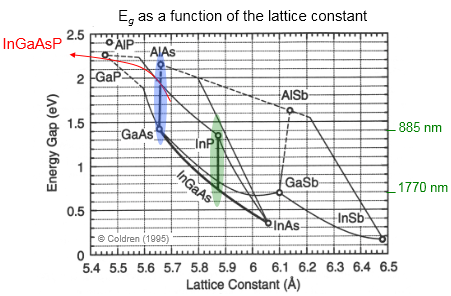
\includegraphics[scale=0.5]{img/image35.png}
			\captionof{figure}{Dipôle}
		\end{wrapfigure}
		Un dipôle électrique est un ensemble de deux charges solidaires de même grandeur et de signes opposés, $+q$ et $-q$ séparées d'une distance $d$.
		
		\subsection{Moment dipolaire $\vec p$}
		Le moment dipolaire est défini comme $\vec p = q\vec d$. C'est un vecteur orienté de la charge négative vers la charge positive.
		
		\subsection{Potentiel et champ autour d'un dipôle}
		Le potentiel dû à un dipôle en un point vaut\footnote{où $\vec{R}$ représente le vecteur joignant le dipôle au point considéré.} :
		\begin{equation}
		V(\vec{R}) = \frac{1}{4\pi\epsilon_0}\frac{\vec{p}.\vec{1_r}}{R^2}
		\end{equation}
		
		\newpage
		\subsection{Force et couple agissant sur un dipôle}
		\begin{wrapfigure}[6]{r}{4cm}
			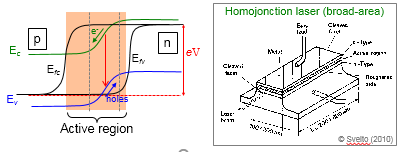
\includegraphics[scale=0.5]{img/image36.png}
			\captionof{figure}{Couple de force sur un dipôle}
		\end{wrapfigure}
		Tout dipôle plongé dans un champ $\vec{E}$ - supposé uniforme - subit un couple\footnote{Démonstration slide 117, page 60.} :
		\begin{equation}
		\vec{\tau} = \vec{p}\times \vec{E}
		\end{equation}
		
		La force agissant sur un dipôle est\footnote{Démonstration slide 119, page 61.} :
		\begin{equation}
		\vec{F} = (\vec{p}.grad)\vec{E}
		\end{equation}
		
		
		
		
		
		\chapter{Milieux diélectriques}
		Il s'agit de matériaux isolats : peu de charges électriques capables de se mouvoir pour donner lieu à des courants (peu ou pas d'$e^-$ libres). On fera l'hypothèse qu'à l'échelle atomique peuvent exister ou apparaître des dipôles qui subirons une polarisation.
		
		
		\section{Comment étendre les équations de Maxwell aux milieux diélectriques ?}
		\subsection{Introduction}
		L'électrostatique dans le vide est basée sur l'idée que $\vec{E}$ est partout défini. On retrouve la force grâce à $\vec{F} = q_0\vec{E}$ et $\vec{E}$ avec $div\ \vec{E} = \frac{\rho}{\epsilon_0}$.\\
		
		Hélas, cela ne fonctionne plus en diélectrique, on ne trouve pas réellement la force sur $q_0$.
		
		\subsection{L'astuce : charges libres et charges de polarisation}
		\subsubsection{Le champ électrique $\vec{E}$ reste défini comme force par unité de charge}
		On conserve ce que l'on a \textit{défini} précédemment :
		\begin{equation}
		\vec{E} = \frac{\vec{F}}{q_0}
		\end{equation}
		
		\subsubsection{Les charges libres sont les sources du problème}
		On considère que les charges autre que $q_0$ continuent à générer un champ : ce sont les \textbf{charges libres}
		\begin{equation}
		div\ \vec{E}_l = \frac{\rho_l}{\epsilon_0}
		\end{equation}
		Mais on ne peut appeler $\vec{E}_l$ \textit{champ électrique} car il ne répond pas à la définition.
		
		\subsubsection{Les charges de polarisation représentent l'influence du diélectrique}
		
		
		Le champ électrique $\vec{E}$ n'est plus directement lié au source. La différence entre $\vec{E}$ et $\vec{E}_l$ donne un troisième champ : $\vec{E}_p$
		\begin{wrapfigure}[15]{r}{4.5cm}
			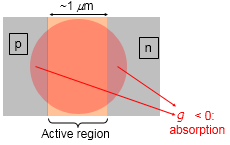
\includegraphics[scale=0.44]{img/image37.png}
			\captionof{figure}{Maxwell pour les diélectriques}
		\end{wrapfigure}
		\begin{equation}
		\vec{E} = \vec{E}_l + \vec{E}_p
		\end{equation}
		On voit que le champ électrique se réduit par rapport au vide, donc que $\vec{E}_p$ s'oppose à $\vec{E}_l$.\\
		Par \textbf{cohérence} on considère des \textit{charges e polarisation} (ou charges liées- qui répondent aussi à Gauss 
		\begin{equation}
		div\ \vec{E}_p = \frac{\rho_p}{\epsilon_0}
		\end{equation}
		
		\subsubsection{La loi de gauss reste mais...}
		Il faut tenir compte de la somme de la \textit{densité de charge libre} et de la \textit{densité de charge de polarisation} :
		\begin{equation}
		\rho = \rho_l + \rho_p
		\end{equation}
		Et l'on peut écrire la loi de Gauss comme précédemment : $div\ \vec{E} = \frac{\rho}{\epsilon_0}$.\\
		
		\prop{En présence de diélectrique, la loi de Gauss reste valable à condition de considérer dans celle-ci la charge totale (somme des charges libres et des charges de polarisation).}\
		
		\section{Matériaux diélectriques et polarisation}
		\subsection{Hypothèse de la polarisation}
		Le champ $\vec{E}$ externe \textit{polarise} les matériaux isolants, c'est-à-dire qu'il oriente préférentiellement les dipôles permanents ou induits.
		
		\subsection{Le champ $\vec{P}$ : polarisation}
		La polarisation est la \textit{densité} de moment dipolaire. C'est la moment dipolaire par unité de volume\footnote{Par exemple, pour $N$ atomes ayant un moment dipolaire $q_e\vec{d}$ on trouve $\vec{P} = Nq_e\vec{d}$}
		\begin{equation}
		\vec{p} = \int_v \vec{P}.d\tau
		\end{equation}
		
		
		\subsection{Potentiel et champ générés par de la matière polarisée}
		Le potentiel dû à un volume de matériau polarisé est identique à celui de charges de surface et de volume (d'un matériau non polarisé.
		\begin{equation}
		V = \frac{1}{4\pi \epsilon_0}\oint_S \frac{\sigma_p}{R}dS + \frac{1}{4\pi\epsilon_0}\int_\tau \frac{\rho_p}{R}d\tau
		\end{equation}
		
		On va comparer deux situations : une avec un matériau dans lequel j'ai des dipôles que je vais pouvoir la décrire avec un champ $\vec{P}$.\\
		Cette situation est équivalente à un problème dans le vide dans lequel j'aurais une densité de polarisation $\rho_p$. Je pourrais imaginer qu'il y a des charges de surfaces.\\
		Dans ce cas $div \vec{E} = \frac{\rho}{\epsilon_0}$ sera toujours d'application. Elles sont équivalentes. Reste à savoir quelle est la relation entre les deux:
		\begin{proof} (pas a connaître)
			Un volume élémentaire $d\tau$ contient un moment dipolaire élémentaire : $dp = P.d\tau$. Par le ch. précédent, le potentiel autour de $\tau$ vaut donc
			\begin{equation}
			V(\vec{R}) = \frac{1}{4\pi\epsilon_0}\int_\tau \frac{\vec{P}.\vec{1_R}}{R^2}d\tau
			\end{equation}
			Comme $grad\ (1/R) = \vec{1_R}/R^2$
			\begin{equation}
			V = \frac{1}{4\pi\epsilon_0}\int_\tau \vec{P}.grad\left(\frac{1}{R}\right).d\tau
			\end{equation}
			En utilisant la propriété $div(f\vec{a}) = fdiv(\vec{a}) + \vec{a}.grad(f)$ on obtient : 
			\begin{equation}
			V_p(\vec{R}) = \frac{1}{4\pi\epsilon_0}\left[\int_v div\left(\frac{\vec{P}}{R}\right)d\tau - \int_V \frac{1}{R}div(\vec{P})d\tau\right]
			\end{equation}
			J'applique Ostrogradsky sur le premier terme :
			\begin{equation}
			V_p(\vec{R}) = \frac{1}{4\pi\epsilon_0}\oint_S \frac{\vec{P}.d\vec{S}}{R} - \frac{1}{4\pi\epsilon_0}\int_V \frac{div\vec{P}}{R}d\tau
			\end{equation}
			En utilisant les relations suivantes :
			\begin{equation}
			\left\{\begin{array}{l}
			V = \frac{1}{4\pi\epsilon_0}\int_\tau \frac{\rho}{R}d\tau\\
			V = \frac{1}{4\pi\epsilon_0}\int_S \frac{\sigma}{R}dS
			\end{array}\right.
			\end{equation}
			On trouve
			\begin{equation}
			V_p(\vec{R}) = \frac{1}{4\pi\epsilon_0}\oint_S \frac{\sigma_p}{R}dS + \frac{1}{4\pi\epsilon_0} \int_\tau \frac{\rho_p}{R}d\tau
			\end{equation}
			Par identification, on montre que le potentiel généré en tout point par un matériau polarisé de polarisation $\vec{P}$ est identique au potentiel électrique qui serait généra par une distribution de charge telle que :
			\begin{equation}
			\left\{\begin{array}{l}
			\sigma_p = \vec{P}.\vec{1_n}\\
			\rho_p = -div\ \vec{P}
			\end{array}\right.
			\end{equation}
		\end{proof}
		
		\section{Champ de déplacement $\vec{D}$ et relation constitutive}
		Pour "simplifier", on introduit le champ de déplacement $\vec{D}$. Pour tenir compte des charges de polarisation, je dois changer $\rho$ 
		\begin{equation}
		div\ \vec{E} = \frac{\rho}{\epsilon_0}\ \ \ \ \text{où} \left\{\begin{array}{l}
		\rho = \rho_l + \rho_p\\
		\rho_p = -div\ \vec{P}
		\end{array}\right.
		\end{equation}
		On trouve ainsi que $div(\epsilon_0\vec{E}) = \rho_l - div\ \vec{P} \Leftrightarrow div(\epsilon_0\vec{E} + \vec{P}) = \rho_l$.\\
		En introduisant le champ $D = \epsilon_0\vec{E} + \vec{P}$
		\begin{equation}
		div\ \vec{D} = \rho_l
		\end{equation}
		Le champ $\vec{D}$ (champ source) ne fait intervenir que la charge libre contrairement au champ $\vec{E}$ (champ effet) qui considère la charge totale\footnote{La seule différence entre les deux est un facteur $\epsilon_0$}.
		\begin{equation}
		\vec{E} = \frac{4}{4\pi\epsilon_0R^2}\vec{1_R}\ \ \ \ \ \ \ \ \ \ \ \ \ \vec{D} = \frac{4}{4\pi R^2}\vec{1_R}
		\end{equation}
		
		\section{Diélectriques linéaires}
		\setcounter{subsection}{1}
		\subsection{Diélectrique linéaire}
		\prop{Un diélectrique est linéaire si sa permittivité est une constante.$$\vec{D} = \epsilon \vec{E}$$}\ \\
		La polarisation est logiquement liée au champ extérieur. Par définition:
		\begin{equation}
		\vec{P} = \chi_e \epsilon_0\vec{E}
		\end{equation}
		On obtient que $\vec{D} = \epsilon_0\vec{E} + \vec{P} = \epsilon_0(1+\chi_e) = \epsilon_0.\epsilon_r.\vec{E} = \epsilon\vec{E}$.\\
		On retrouve les notation du cours de \textit{Physique Générale} ou $\epsilon_0$ est la permittivité du vide, $\epsilon_r$ est la permittivité relative et $\chi_e$ la susceptibilité électrique.\footnote{En pratique $\epsilon_r \geq 1$ (ou $\epsilon \geq \epsilon_0$), c'est-à-dire que pour un même champ $\vec{D}$, le champ $\vec{E}$ est plus faible en présence d'un diélectrique que dans le vide.}
		
		
		\subsection{Diélectriques linéaires homogène}
		Un diélectrique est \textbf{homogène} si sa permittivité est constante dans l'espace. On peut dès lors montrer que la densité de charge de polarisation $\propto$ densité de charge libre :
		\begin{equation}
		\rho_p = -div\vec{P} = -div(\chi_e\epsilon_0\vec{E}) =-div\left(\frac{\chi_e\epsilon_0}{\epsilon}\vec{D}\right) = -\frac{\chi_e\epsilon_0}{\epsilon}div(\vec{D}) = -\frac{\chi_e}{\epsilon_r}\rho_l
		\end{equation}
		Sa densité de charge totale vaut alors :
		\begin{equation}
		\rho = \rho_l + \rho_p = \left(1-\frac{\chi_e}{\epsilon_r}\right)\rho_l = \frac{\rho_l}{\epsilon_r}
		\end{equation}
		S'il n'y a pas de charge libre à l'intérieur du diélectrique, il n'y aura pas de polarisation en volume : $\rho_p = 0$.\\
		
		On en conclut que la théorie des diélectriques linéaires et homogènes est similaire à celle des champs dans le vide, \textit{à condition d'y remplacer $\epsilon_0$ par $\epsilon$}.
		\begin{center}
			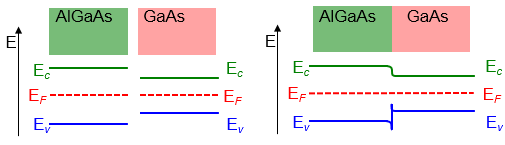
\includegraphics[scale=0.6]{img/image38.png}
			\captionof{figure}{Tableau récapitulatif}
		\end{center}
		\setcounter{section}{5}
		
		\section{Conditions aux limites}
		Comme précédemment, on va retrouver une discontinuité entre les champs $\vec{D}$ et $\vec{E}$ de part et d'autres d'une surface chargée. \textit{(Cf. slide T43-45, page 85-87)}
		
		\section{Énergie dans les diélectriques linéaires}
		Pour rappel, on avait obtenu dans le vide $w_e = \frac{1}{2}\epsilon_0E^2$. En présence de diélectriques linéaires, celle-ci vaut maintenant en tout point\footnote{Démonstration page 88-89.} :
		\begin{equation}
		w_e = \frac{1}{2}\vec{D}.\vec{E} = \frac{1}{2}\epsilon E^2
		\end{equation}
		Cela peut également s'écrire\footnote{Comme $\vec{D} = \epsilon_0\vec{E} + \vec{P}$} $w_e = \frac{1}{2}\epsilon_0E^2 + \frac{1}{2}\vec{P}.\vec{E}$ ou le deuxième terme est l'énergie additionnelle qui doit être fournie par les sources pour établir le champ $\vec{E}$ dans un milieu diélectrique : c'est l'énergie supplémentaire requise pour \textit{polariser} le diélectrique.
		
		\section{Condensateur plan avec diélectrique}
		\subsection{Calcul du champ}
		\begin{wrapfigure}[9]{l}{6cm}
			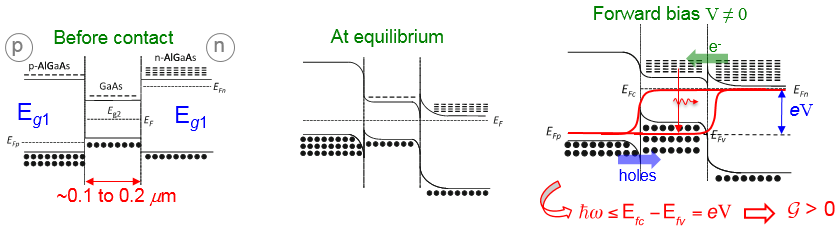
\includegraphics[scale=0.45]{img/image39.png}
			\captionof{figure}{Condensateur plan avec diélectrique}
		\end{wrapfigure}
		En présence d'un champ extérieur (charges sur les armature) les diélectrique se polarise :(charge superficielle de polarisation apparaissant en face des armatures et champ électrique "induit" opposé au champ initial).\\
		Le champ initial vaut $\vec{E}_0 = \frac{\sigma_l}{\epsilon_0}\vec{1_z}$. Compte-tenu de $\vec{\sigma}_p = \vec{P}.\vec{1_n}$, le champ total est:
		\begin{equation}
		\vec{E} = \vec{E_0} + \vec{E_p} = \frac{\sigma_l - P}{\epsilon_0}\vec{1_z}
		\end{equation}
		Les charges de polarisation sont, sur chaque armature, de signe opposé aux charges libre et créent bien un champ opposé à $\vec{E_0}$.\\
		
		Pour un diélectrique linéaire $P = \chi_e\epsilon_0 E$ on trouve que le champ est réduit d'un facteur $\epsilon_r$ :
		\begin{equation}
		E = \frac{\sigma}{\epsilon_0}\frac{1}{1+\chi} = \frac{\sigma_l}{\epsilon_0}\frac{1}{\epsilon_r} = \frac{\sigma_l}{\epsilon}
		\end{equation}
		
		\subsection{Calcul de la capacité}
		La ddp entre les armatures est $V = E.d = \frac{\sigma_l d}{\epsilon}$ et la charge totale $Q = \sigma_l.A$. La capacité vaut dès-lors :
		\begin{equation}
		C = \frac{Q}{V} = \epsilon_r\frac{\epsilon_0 A}{d} = \frac{\epsilon A}{d}
		\end{equation}
		La capacité est donc multipliée par le facteur $\epsilon_r$ dans le cas d'un diélectrique homogène par rapport à sa valeur dans le vide.
		
		\subsection{Force latérale due à l'effet de bord}
		Petit cas d'école suffisamment détaillé à la page 92-93. 
		
		\section{Expression générale du coefficient de capacité}
		Reprenons notre condensateur en supposant que l'espace entre les armatures est entièrement rempli par un diélectrique linéaire et  homogène de permittivité $\epsilon$. La forme "non" générale bien connue est $C = \frac{Q}{V}$. Cette charge $Q$ est bien la \textit{charge libre} et est donc lié au champ de déplacement. L'expression générale sera donc :
		\begin{equation}
		C = \dfrac{\oint_s \vec{D}.\vec{dS}}{- \int_L \vec{E}.d\vec{l}}
		\end{equation}
		Ou encore :
		\begin{equation}
		C = \dfrac{\oint_s \epsilon\vec{E}.\vec{dS}}{- \int_L \vec{E}.d\vec{l}}
		\end{equation}
		\subsection{Exemple : condensateur cylindrique}
		Grand classique du cours de \textit{Physique Générale} : Cf. slide T58 et page 95.
		\begin{equation}
		C = \dfrac{2\pi \epsilon L}{ln\left(\frac{b}{a}\right)}
		\end{equation}
		
		
		\chapter{Milieux conducteurs (effet résistif)}
		Dans certains matériaux, l'application d'une champ $\vec{E}$ externe provoque un mouvement de charges électriques, soit un courant.\\
		Ce sont ces \textit{charges libres} qui caractérisent les conducteurs.
		
		\section{Tension et courant}
		Le courant est un débit de charge $I = \frac{\Delta Q}{\Delta t}$. Si celui-ci n'est pas constant, on peut considérer sa valeur instantanée.
		\begin{equation}
		I(t) = \lim\limits_{\Delta t \rightarrow 0} \frac{\Delta Q}{\Delta t} = \frac{dQ}{dt}
		\end{equation}
		Il est plus courant lorsqu'on travaille localement d'utiliser la \textit{densité de courant}, c'est-à-dire le courant traversé par unité de surface : $J = \frac{I}{S}$. Ceci permet de redéfinir le courant de la sorte :
		\begin{equation}
		I = \int_S \vec{J}.d\vec{S}
		\end{equation}
		Une autre façon de définir $\vec J$ est de multiplier la densité de volume par la vitesse : $\vec{J} = \rho \vec{u}$.
		
		\section{Relation constitutive : loi d'Ohm locale}
		\subsection{Loi d'Ohm locale}
		Imposer un champ électrique sur des charges libres fait apparaître une densité de courant $\vec{J} \neq 0$. Ceci est modélisé de façon linéaire :
		\begin{equation}
		\vec{J} = \sigma\vec{E}
		\end{equation}
		où $\sigma$ est la \textbf{conductivité} [$\Omega^{-1}m^{-1}$]. Ceci est l'expression de la \textit{loi d'Ohm locale}. \\
		\textbf{Attention !} La densité surfacique de charge sera noté $\zeta$ et la conductivité $\sigma$, ne pas confondre!
		\subsection{Conductivité et résistivité}
		La résistivité est l'inverse de la conductivité, elle s'exprime donc en [$\Omega m$] := $\rho = \frac{1}{\sigma}$.\\
		\textbf{Attention !} Ne pas la confondre avec la densité volumique de charge $\rho_v$.\\
		Ces facteurs dépendent assez fortement de la température :
		\begin{equation}
		\rho = \rho_0[1+\alpha(T-T_0)]
		\end{equation}
		où $\rho_0, T_0$ sont les valeurs de références et $\alpha$ le coefficient de température.
		
		
		\section{Coefficient de résistance}
		\subsection{Conducteurs soumis à une différence de potentiel}
		\begin{wrapfigure}[11]{r}{4.5cm}
			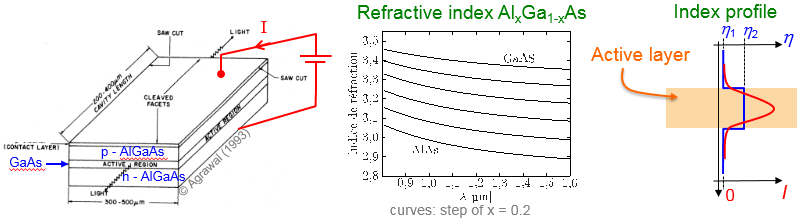
\includegraphics[scale=0.44]{img/image40.png}
			\captionof{figure}{Matériau conducteur entouré d'un isolant}
		\end{wrapfigure}
		Soit un matériau conducteur ($\sigma$) entouré par du vide (isolant parfait). En appliquant une ddp (moyen externe) je crée un champ $\vec{E}$ qui va causer l'apparition d'une densité de courant $\vec{J} = \sigma\vec{E}$.\\
		S'il n'y a pas d'accumulation de charge $\frac{d\rho_v}{dt} = 0$ et l'équation de continuité de charge vaut :
		\begin{equation}
		\oint_S \vec{J}.d\vec{S} = 0
		\end{equation}
		Vu qu'aucun courant ne peut s'échapper, le courant total traversant deux surfaces quelconques $A'$ et $A$ sera identique.
		\begin{equation}
		\int_A \vec{J}.d\vec{S} = \int_{A'} \vec{J}.d\vec{S} = I
		\end{equation}
		Ceci est vrai $\forall$ forme du conducteur. Le conducteur qui n'est plus équipotentiel présente bien des surfaces équipotentielles.
		
		\subsection{Coefficient de résistance}
		Connaissant l'expression de la ddp $V = -\int_L \vec{E}.\vec{dl}$, la définition de $I = \int_A \vec{J}.d\vec{S} = \int_A \sigma\vec{E}.d\vec{S}$ ainsi que la loi d'Ohm, on peut définir le \textit{coefficient de résistance } $R$ :
		\begin{equation}
		R = \dfrac{-\int_L \vec{E}.\vec{dl}}{\int_A \sigma\vec{E}.d\vec{S}}
		\end{equation}
		Ce coefficient traduit la disposition géométrique du milieu.
		
		
		\section{Temps de relaxation}
		En principe un métal est un bon conducteur et un diélectrique un bon isolant. Mais ceux-ci peuvent être le siège d'un effet diélectrique et résistif simultanément.\\
		Soit un milieu linéaire et homogène ($\epsilon, \sigma$). Pour une densité volumique de charge $\rho_v$ :
		\begin{equation}
		div\ \vec{E} = \frac{\rho}{\epsilon}
		\end{equation}
		En utilisant la loi d'Ohm locale et l'équation de continuité $div\ \vec{J} +\frac{\partial \rho_v}{\partial t} = 0$, on obtient une équation différentielle en $\rho_v$ :
		\begin{equation}
		\frac{\partial \rho_v}{\partial t} + \frac{\sigma}{\epsilon}\rho_v = 0
		\end{equation}
		La solution donne la variation temporelle de $\rho_v$ au départ de $\rho_{v,0}$
		\begin{equation}
		\rho_v(t) = \rho_{v,0}e^{-\left(\frac{\sigma}{\epsilon}\right)t}
		\end{equation}
		La charge de volume diminue pour se retrouver à la surface du matériaux. La \textbf{temps de relaxation} est le constante $t_r = \dfrac{\epsilon}{\sigma}$. C'est la durée nécessaire pour que $\rho_v$ diminue de $36.8\%$.\\
		Dans le cuivre $t_r = 1,5.10^{-19}s$. Toute $\rho_v$ qui apparaît disparaît donc quasi instantanément. Considérer $\rho_v =0$ dans un conducteur est donc raisonnable.
		
		\section{Conditions aux limites}
		Même raisonnement que précédemment (Cf. syllabus p 109).
		
		\section{Aspects microscopiques : courant de conduction (pas connaître les formules)}
		Dans un atomes, les électrons de valences vont subir une force $\vec{F} = q\vec{E}$ en présence d'un champ électrique à une \textit{vitesse de dérive}.
		
		\subsection{Expression de la densité de courant}
		\begin{wrapfigure}[11]{r}{3cm}
			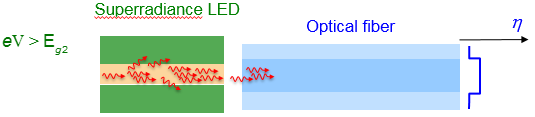
\includegraphics[scale=0.44]{img/image41.png}
			\captionof{figure}{Courant au travers d'une surface}
		\end{wrapfigure}
		S'il y a $N$ particules par unité de volume, la densité de charge vaut $\rho_v = Nq$. Comme pour le cours de \textit{Physique Générale}, les particules parcourent une distance $\Delta L = u\Delta t$ durant un temps $\Delta t$.\\
		La quantité de charge traversant la surface vaut donc (en vectorielle pour toute généralité) :
		\begin{equation}
		\Delta Q = Nq\vec{u}.\Delta\vec{S}\Delta t
		\end{equation}
		Le courant vaut dès lors $Nq\vec{u}.\Delta S$, ou encore avec la densité de courant $\vec{J} = Nq\vec{u} = \rho_v \vec{u}$. Ceci se généralise facilement dans le cas à plusieurs type de charges à l'aide d'une sommation.
		
		
		\subsubsection{Cas particulier d'un conducteur métallique}
		Ici les charges sont les $e^-$ libres. Les charges positives des noyaux restent immobiles par rapport au volume du conducteur (pas de rôle dans le courant). Comme il y a priori deux types de charges\footnote{La vitesse relative des électrons par rapport au conducteur $\vec{v_e}$ est aussi appelé \textit{vitesse de dérive} $\vec{v_d}$.} : 
		\begin{equation}
		\vec{J} = \rho_{v,e}\vec{v_e} + \rho_{v,p}\vec{v_p}
		\end{equation}
		Comme $\vec{v_p} = \vec{0}$, la densité de courant se réduit à $\vec{J} = \rho_e\vec{v_e} = N_eq_e\vec{v_e}$.\\
		Le déplacement des $e^-$ n'empêche pas la neutralité du conducteur dans son ensemble ($\rho_{v,e} + \rho_{v,p} = 0$). Un courant peut donc exister dans un conducteur non chargé.
		
		\subsection{Courant de conduction >< courant de convection}
		La loi d'Ohm locale semble montrer que les électrons n'accélèrent pas mais évoluent à vitesse constante ce qui est en opposition avec $f=ma$. Ceci s'explique car $\vec{v_d}$ ne représente pas la vitesse individuelle des charges.
		
		
		\begin{description}
			\item[Courant de conduction] : Mouvement d'ensemble des électrons libres à l'intérieur d'un conducteur. C'est le "courant" usuel qui suit la loi d'Ohm. C'est le nuage d'électron pris dans son ensemble.
			\item[Courant de convection] : Déplacement de matière chargée par exemple électrons dans les tubes cathodiques. Ne suit pas la loi d'Ohm. Ce sont les électrons pris dans le vide.
		\end{description}
		
		\prop{Dans un conducteur, le débit de charges est un courant de conduction : il résulte d'un mouvement d'ensemble des porteurs de charges libres de se déplacer.}
		
		\subsection{Vitesse des charges = vitesse de dérive}
		Chaque $e^-$ rentre en collision dans le cristal et cela arrive souvent : c'est le mouvement brownien qui correspond à la situation ou il n'y a pas de courant. \\
		En moyenne, l'$e^-$ parcourt une distance entre deux collision : le libre parcours moyen. J'ai donc également un temps moyen entre deux collisions.
		\begin{equation}
		\lambda = v_{th}.t_c
		\end{equation}
		Ici $f=ma$ est bien vérifiée, la vitesse de dérive est la vitesse moyenne du nuage d'électrons ou les électrons rentrent toujours en collision avec le cristal. La vitesse de la loi d'Ohm est donc la vitesse du nuage.\\
		On définira ainsi la mobilité comme le coefficient de $\propto$ entre $v$ et $E$
		\begin{equation}
		\vec{v_d} = \mu_e\vec{E}
		\end{equation}
		
		En prenant des données chiffrés, on remarque que le déplacement du nuage\footnote{$\vec{v_d}$ est très lente.} est très lent ($cl/h$ pour de bons conducteurs) mais le déplacement des électrons est très rapide.
		
		\section{Puissance dissipée : effet Joule}
		Le travail nécessaire pour déplacer $dQ$ dans un potentiel vaut $dW = V dQ$. Comme $P = \frac{dW}{dt}$ :
		\begin{equation}
		P = IV
		\end{equation}
		La puissance dissipé vaudra dès lors $RI^2 = V^2/R$.\\
		
		La force par unité de volume vaut $\vec{f} = \rho_v\vec{E}$. Comme $p = \vec{f}.\vec{v}$ la puissance dissipée en formulation locale :
		\begin{equation}
		p_{joule} = \rho\vec{E}\vec{v} = \vec{J}.\vec{E} = \sigma E^2
		\end{equation}
		Comme l'$E_c = cste$ toute l'énergie se retrouve dissipée en chaleur.\\
		La puissance totale dissipée peut s'obtenir en intégrant la densité de puissance sur le volume du conducteur.
		\begin{equation}
		P_{joule} = \int_V \vec{J}.\vec{E}d\tau
		\end{equation}
		\section{Exemples de calcul de résistance}
		Voir syllabus page 121-122, slides 39-42.
		
		\section{Analogie entre résistance et capacité}
		On peut remarqué que $R$ et $C$ ont des formulations proches :
		\begin{equation}
		\left\{\begin{array}{l}
		R = \dfrac{I}{V} = \dfrac{-\int_L \vec{E}\vec{dl}}{\int_S \sigma\vec{E}d\vec{S}}\\
		C = \dfrac{Q}{V} = \dfrac{\oint_S \vec{E}d\vec{S}}{-\int_L \vec{E}.\vec{dl}}
		\end{array}\right.
		\end{equation}
		On remarque que si l'on connaît la résistance, on peut calculer la capacité sans recalculer une intégrale et inversement.
		\begin{equation}
		RC = \dfrac{\epsilon}{\sigma}
		\end{equation}
		\textbf{Attention !} Ne pas se tromper en considérant $R$ et $C$ ! L'exemple page 124 est pertinent.
		
		\section{Équations de Maxwell et loi des nœuds}
		\textit{La somme (algébrique) des courants entrants dans un nœud est nulle} : cela se justifie par les equations de Maxwell. 
		\begin{proof}\ \\
			L'équation de continuité sous forme locale est $div\ \vec{J} = -\frac{\partial \rho_v}{\partial t}$ et appliquons la au nœud ci-dessous.
			\begin{center}
				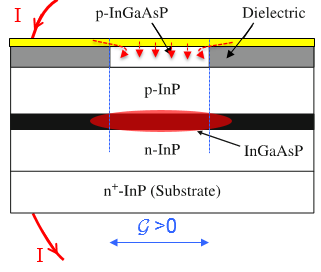
\includegraphics[scale=0.30]{img/image42.png}
				\captionof{figure}{Nœud}
			\end{center}
			\begin{equation}
			\sum_j I_j + \int_{\text{Si isolante}} \vec{J}.d\vec{S} = -\frac{dQ}{dt}
			\end{equation}
			En considérant un isolant parfait, la densité de courant est nulle ($\vec{J} = \sigma\vec{E}$) : le terme intégral l'est également.\\
			A l'intérieur d'un bon conducteur, la densité volumique est nulle : la charge totale\footnote{Charges positives et négatives confondue} est aussi nulle tout comme sa dérivée\footnote{Cela traduit le fait qu'il n'y a pas d'accumulation de charges.}.
			\begin{equation}
			\frac{dQ}{dt} = \frac{d}{dt}\int_\tau \rho_v d\tau = 0
			\end{equation}
			On retrouve bien que la somme algébrique des courants entrant dans un nœud est nulle
			\begin{equation}
			\sum_j I_j = 0
			\end{equation}
		\end{proof}
		
		\section{Loi des mailles et force électromotrice}
		\subsection{Justification de la loi des mailles}
		Démontrons la loi des mailles :
		\begin{proof}
			\ \\
			En statique, d'après la deuxième loi de Maxwell
			\begin{equation}
			\oint_C \vec{E}.\vec{dl} = 0
			\end{equation}
			Combinons cela à la relation liant $\vec E$ et $V$ :
			\begin{equation}
			\vec{E} = -grad\ V
			\end{equation}
			Cela signifie que la somme des ddp le long de toute maille fermée est nulle
			\begin{equation}
			\sum_{circuit} \Delta V_i = 0
			\end{equation}
		\end{proof}
		
		\subsection{Rôle du générateur dans un circuit}
		\subsubsection{Le générateur : un composant qui viole les équations de Maxwell}
		\begin{wrapfigure}[15]{r}{4cm}
			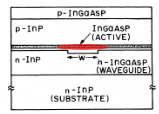
\includegraphics[scale=0.5]{img/image43.png}
			\captionof{figure}{Représentation imagée de la circulation des charges dans un circuit}
		\end{wrapfigure}
		Dans un générateur, les charge ne vont pas du "+" au "-" puisque le courant doit circuler en boucle fermer il doit aller du "-" au "+" dans le générateur : viol des équations ; les charges vont à priori "remonter" le champ électrique. Les charges vont à contre-sens du chap $E$ par rapport au circuit extérieur : la source communique de l'énergie potentielle aux charges.\\
		
		Que se passe-t-il dans une pile ? Il va y avoir un phénomène autre électromagnétique qui entretient la différence de potentiel. Comme ici c'est chimique (et donc d'origine externe), ce n'est pas régi par Maxwell. 
		
		
		\subsection{Modélisation du générateur : force électromotrice}
		On va supposer qu'il existe dans un générateur une force de sens contraire à $\vec E$ qui a pour effet de "remonter le potentiel des charges" ($- \rightarrow +$), force notée $\vec{f_s}$.
		La force nette dans le générateur vaut alors\footnote{$\vec{f_s}$ n'agit que dans la source alors que $\vec{E}$ est présent tout au long du contour.} :
		\begin{equation}
		\vec{f_{tot}} = \vec{f_s} + \vec{E}
		\end{equation}
		
		\subsubsection{Force électromotrice}
		Il s'agit de la circulation de la force nette sur toute la longueur du circuit
		\begin{equation}
		\mathcal{E} = \oint_C \vec{f_{tot}}.\vec{dl}
		\end{equation}
		Comme $\vec{f_s}$ est nulle en dehors de la pile, on peut ré-écrire :
		\begin{equation}
		\mathcal{E} = \oint_C \vec{f_s}.\vec{dl} + \underbrace{\oint_c \vec{E}.\vec{dl}}_{=0} = \int_a^b \vec{f_s}.\vec{dl}
		\end{equation}
		La fem peut être interprétée comme le travail par unité de charge fourni par la source. Dans une pile $\vec{f_s}$ est la force nécessaire pour séparer les + des - et de les placer sur les bornes en surmontant la répulsion des charges qui s'y trouvent déjà.
		
		\subsection{Cas de la source idéale}
		Pour qu'un courant circule, il suffit que les potentiels aux bornes de la source restent constants c'est-à-dire si le champ d'origine externe neutralise le champ électrostatique.
		\begin{equation}
		\vec{E}_{gen} = -\vec{f_s}
		\end{equation}
		On a dans ce cas 
		\begin{equation}
		V_{ab} = V_b - V_a = -\int_a^b \vec{E}.\vec{dl} = \int_a^b \vec{f_s}.\vec{dl}
		\end{equation}
		La différence de potentiel aux bornes de la source vaut alors la fem :
		\begin{equation}
		V_{ab} = \int_a^b \vec{f_s}.\vec{dl} = \mathcal{E}
		\end{equation}
		L'équation d'une source idéale sera dès lors $V = \mathcal{E}$.\\
		\textbf{Attention !} Une ddp est la circulation du champ $E$, soit un travail effectué par $E$ pour faire circuler les charges et dissipée en chaleur alors que la fem est une énergie/travail d'origine externe fourni(e) par la source.
		
		\subsubsection{Cas de la source non idéale}
		Si $\sigma_{cond} \neq \infty$, déplacer les charges dans la source demande un travail additionnel. Dans la source, $I$ est dû au déplacement des ions.
		\begin{equation}
		\vec{v}_{ions} = \mu_{ions}(\vec{f_s}+\vec{E})
		\end{equation}
		La densité de courant dans la pile sera de la forme
		\begin{equation}
		\vec{J} = \sigma_{ions}(\vec{f_s}+\vec{E})
		\end{equation}
		Dans la pile, on a toujours
		\begin{equation}
		\vec{f_s} = -\vec{E} + \dfrac{\vec{J}}{\sigma_{ions}}
		\end{equation}
		La fem vaut dès lors
		\begin{equation}
		\mathcal{E} = \int_a^b \vec{f_s}.\vec{dl} = -\int_a^b \vec{E}.\vec{dl} + \int_a^b \dfrac{\vec{J}}{\sigma_{ions}}.\vec{dl}
		\end{equation}
		Le premier terme est la ddp entre $a$ et $b$ tandis que le deuxième peut s'écrire $R_{out}I$. On a donc :
		\begin{equation}
		\mathcal{E} = V_{ab} + R_{out}I
		\end{equation}
		La fem (travail par unité de charge) doit compensé non seulement la dissipation dans le circuit par l'effet joule mais aussi la résistance interne du générateur qui s'oppose à la circulation du courant dans celui-ci.
		
		
		
		
		
		
		
		
		
		
		
		
		
		
		
		\chapter{Magnétostatique}
		\section{Introduction}
		La force de Lorentz se compose d'une force électrique générée par un champ $\vec{E}$ ainsi que d'une force magnétique.
		\begin{equation}
		\vec{F} = q(\vec{E} + \vec{v}\times\vec{B})
		\end{equation}
		\begin{wrapfigure}[9]{r}{3cm}
			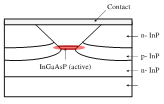
\includegraphics[scale=0.5]{img/image44.png}
			\captionof{figure}{Force sur un élément de courant}
		\end{wrapfigure}
		où $\vec{F_m} = q\vec{v}\times\vec{B}$ est la force magnétique décrit au moyen du champ magnétique $\vec{B}$ qui lui-même est produit par des charges en \textit{mouvement}.\\
		On peut voit $\vec{v}$ comme la vitesse de dérive des électrons, par exemple en mouvement dans un fil. Chaque $e^-$ subira la force magnétique $q_e(\vec{v}_d \times B)$.\\
		Sur un volume $d\tau$, la force élémentaire correspondante sera $d\vec{F} = N_ed\tau q_e(\vec{v}_d\times\vec{B})$. En introduisant la densité de courant : $d\vec{F} = (\vec{J}\times\vec{B})$ et que celle-ci est uniforme $d\vec{F} = \vec{J}\times\vec{B}.A.dl$. Comme $\vec{J} = \frac{I}{A}\vec{1_l}$ on trouve :
		\begin{equation}
		d\vec{F} = I \vec{dl}\times \vec{B}
		\end{equation}
		Ce qui est la force par unité de longueur du fil\footnote{On doit voir le courant comme un "vecteur" en opposition à la charge ponctuelle.}. 
		L'intensité et la direction de la force dépend du mouvement de la charge.
		
		\section{Le champ magnétique}
		Les équations de Maxwell pour la magnétostatique dans la vide sont :
		\begin{equation}
		\left\{\begin{array}{l}
		div\ \vec{B} = 0\\
		rot\ \vec{B} = \mu_0\vec{J}
		\end{array}\right.\ \ \ \ \ \ \ \left\{\begin{array}{l}
		\oint_S \vec{B}.d\vec{S} = 0\\
		\oint_C \vec{B}.\vec{dl} = \mu_0I
		\end{array}\right.
		\end{equation}
		Pour récapituler : \textit{charges en mouvement $\rightarrow$ courant\footnote{On supposera ici que les courants sont constants dans le temps.} $\rightarrow$ champ magnétique.}\\
		
		La divergence de $\vec{B}$, en comparaison avec celle de $\vec{E}$ nous montre qu'il n'existe pas de charge magnétique d'où les lignes de champ de $\vec{B}$ pourraient sortir: les lignes de champs forment des boucles ou s'étendent jusqu'à l'infini.\\
		Le rotationnel donne le lien entre $\vec{B}$ et $I$.
		
		
		
		\section{Exemples de champ magnétique}
		La symétrie permet de déterminer les composantes de $\vec{B} \neq \vec 0$ pour ensuite applique la loi d'Ampère\footnote{Aussi appelée loi d'Oersted en version intégrale)}
		
		\subsection{Conducteur rectiligne infini}
		\begin{wrapfigure}[4]{l}{3cm}
			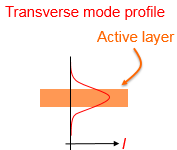
\includegraphics[scale=0.3]{img/image45.png}
			\captionof{figure}{Champ $\vec{B}$ d'un conducteur infini}
		\end{wrapfigure}
		Le courant $I$ est constant dans un fil rectiligne $\rightarrow$ les lignes de champ magnétiques sont des cercles : $\vec{B} = B_\phi \vec{1_\phi}$. Appliquons  Ampère : \\
		$\oint_C \vec{B}.\vec{dl} = B_\phi \oint dl = B_\phi.2\pi r = \mu_0I$, ce qui nous donne :
		\begin{equation}
		\left\{\begin{array}{l}
		\vec{B} = \dfrac{\mu_0 I r}{2\pi b^2}\vec{1_\phi}\ \ \ \ \ r < b\\
		\vec{B} = \dfrac{\mu_0I}{2\pi r}\vec{1_\phi}\ \ \ \ \ \ \ r > b
		\end{array}\right.
		\end{equation}
		
		
		\subsection{Solénoïde infini}
		\begin{wrapfigure}[9]{r}{1.9cm}
			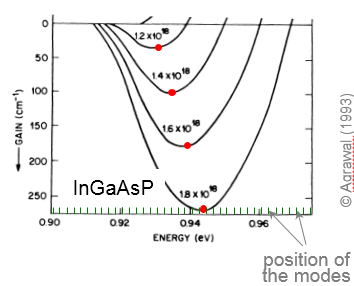
\includegraphics[scale=0.2]{img/image46.png}
			\captionof{figure}{Solénoïde}
		\end{wrapfigure}
		
		La loi d'Ampère permet d'établir que le champ est uniforme à l'intérieur du solénoïde et nul à l'extérieur.
		\begin{equation}
		\left\{\begin{array}{l}
		\vec{B} = n\mu_0 I \vec{1_z}\ \ \ \text{à l'intérieur}\\
		0 \ \ \ \ \ \ \ \ \ \ \ \ \ \ \ \ \ \text{à l'extérieur}
		\end{array}\right.
		\end{equation}
		où $n$ est le nombre de spires par unité de longueur.\\
		Pour le solénoïde fini, le champ est non nul à l'extérieur, les lignes de champ devant se refermer.
		
		\subsection{Tore}
		Un tore est une bobine refermée sur elle-même: symétrie cylindrique implique que le champ aura seulement une composante en $\phi$\footnote{Utiliser Biot-Savart pour s'en convaincre.}. On peut dès lors appliquer Ampère et trouver le champ à l'intérieur :
		\begin{equation}
		\vec{B} = \frac{\mu_0 NI}{2\pi r}\vec{1_\phi}
		\end{equation}
		ou $N$ est le nombre total de spires. Le champ est nul à l'extérieur.
		
		\section{Le potentiel vecteur magnétique}
		La divergence d'un rotationnel est toujours nulle. Comme $div\ \vec{B} = 0$ on peut imaginer un vecteur $\vec A$ satisfaisant :
		\begin{equation}
		\vec{B} = rot\ \vec{A}
		\end{equation}
		où $\vec{A}$ est le \textit{potentiel vecteur magnétique} (ou "potentiel vecteur")\footnote{On peut voir cette expression comme "l'équivalent" de $\vec{E} = -grad\ V$ en électrostatique.}.\\
		
		En électrostatique, $V$ n'était défini qu'à une constante près. Comme on ne connait que $rot\ \vec{A}$, celui-ci n'est défini qu'à une "constante vectorielle" près. \\
		Une fonction dont le rotationnel s'annule est le gradient de quelque chose, ici le gradient d'un potentiel scalaire :
		\begin{equation}
		\vec{A'} = \vec{A} + grad\ \Psi
		\end{equation}
		On peut profiter de ceci pour  imposer $div\ \vec{A} = 0$\footnote{On impose bien un potentiel nul à l'infini, alors pourquoi pas ça ?}.\\
		
		Que devient la $4^e$ équation de Maxwell $rot\ \vec{B} = \mu_0J$ ?
		\begin{equation}
		rot(rot\ \vec{A}) = \mu_0\vec{J}
		\end{equation}
		Comme $rot(rot\ \vec{A}) = grad(div\ \vec{A})-\Delta \vec{A}$ et la divergence de $\vec{A}$ est nulle, on obtient :
		\begin{equation}
		\Delta \vec{A} = -\mu_0\vec{J}
		\end{equation}
		où $\Delta$ est le Laplacien. L'équation du potentiel vecteur est équivalent à trois équations de Poisson :
		\begin{equation}
		\left\{\begin{array}{l}
		\Delta A_x = -\mu_0J_x\\
		\Delta A_y = -\mu_0J_y\\
		\Delta A_z = -\mu_0J_z
		\end{array}\right.
		\end{equation}
		Nous connaissons la solution de l'équation de Poisson pour l'électrostatique : $V = \frac{1}{4\pi\epsilon_0}\int_\tau \frac{\rho}{R}d\tau$. Par analogie, la solution sera (sous forme vectorielle) :
		\begin{equation}
		\vec{A} = \frac{\mu_0}{4\pi}\int_\tau\frac{\vec{J}}{R}d\tau
		\end{equation}
		Deux cas particuliers sont renseignés dans les slides (T31, 32) et (ancien) syllabus page 74.Le potentiel vecteur est globalement orienté comme les courants.\\
		
		Le flux magnétique voit également son expression modifiée : $\Phi = \int_S \vec{B}.d\vec{S}$ où $\vec{B} = rot\ \vec{A}$. Par Stokes, on trouve que le flux à travers une surface est la circulation du potentiel vecteur sur le contour fermé s'appuyant sur la surface.
		\begin{equation}
		\Phi = \int_S rot\ \vec{A}.d\vec{S} = \oint_C \vec{A}.\vec{dl}
		\end{equation}
		La vraie utilité du potentiel vecteur apparaîtra lors de l'étude des champs variables.
		
		
		\section{Formule de Biot-Savart}
		Une longue démonstration (non vue au cours et pas à connaître) nous donne la formule de Biot-Savart :
		\begin{equation}
		\vec{B} = \dfrac{\mu_0I}{4\pi}\int_\tau \dfrac{\vec{J}\times\vec{1_R}}{R^2}d\tau
		\end{equation}
		Elle permet d'obtenir le champ magnétique à partir des courants. Pour un fil, on aura $\vec{J} = I\vec{dl}$.
		
		\section{Exemples de potentiel vecteur}
		Les calculs sont dans le syllabus, ce qui est important c'est de voir que le potentiel vecteur est orienté dans le même sens que le courant (En $\vec{1_z}$ pour le fil en 5.6.1) 
		
		\section{Dipôle magnétique}
		Un dipôle magnétique est une boucle circulaire et filiforme parcourue par un courant $I$. On ne s'intéresse ici qu'aux cas à grande distance par rapport au rayon de la boucle.\\
		Le champ dû à un dipôle magnétique est (démonstration non vue en cours) :
		\begin{equation}
		\vec{B} = \frac{\mu_0 Ib^2}{4R^3}(2\cos\theta \vec{1_R} + \sin\theta \vec{1_\theta}),\ \ \ \ \ \vec{A} = \frac{\mu_0 I b^2}{4R^2}\sin\theta\vec{1_\phi}
		\end{equation}
		\begin{center}
			\includegraphics[scale=0.5]{img/image48.png}
			\captionof{figure}{Champ électrique et magnétique des dipôles}
		\end{center}
		Le moment dipolaire $m$ est le produit du courant par la surface de la boucle :
		\begin{equation}
		\vec{m} = m.\vec{1_z} = I\pi b^2.\vec{1_z} = IS\vec{1_z}
		\end{equation}
		Le champ d'un dipôle vaut :
		\begin{equation}
		\vec{B} = \frac{\mu_0 m}{4\pi R^3}(2\cos\theta\vec{1_R} + \sin\theta \vec{1_\theta})
		\end{equation}
		A grande distance, ce champ est identique à celui du dipôle électrique.
		
		
		\section{Forces et couples sur des courants}
		L'élément de force vu au début de chapitre étant $d\vec{F} = I \vec{dl}\times\vec{B}$, la force totale sur une boucle parcourue de courant est :
		\begin{equation}
		\vec{F} = \oint_C I \vec{dl}\times\vec{B}
		\end{equation}
		où le champ $\vec{B}$ est celui produit par un autre courant : $\vec{F_{12}} = \oint_{C_2} I_2\vec{dl_2}\times\vec{B_1}$. Si le champ est \textbf{uniforme} la force totale sur un circuit fermé est toujours nulle :
		\begin{equation}
		\vec{F} = I \oint \vec{dl}\times\vec{B} = I\left(\oint \vec{dl}\right) \times \vec{B} = 0
		\end{equation}
		mais le champ uniforme produira cependant un couple sur le circuit.
		\begin{center}
			\includegraphics[scale=0.8]{img/image49.png}
			\captionof{figure}{Couple sur une boucle de courant}
		\end{center}
		Les forces sur les côtés de longueur $a$ sont alignées et opposée : pas de couple. Sur les côtés $b$ elle sont opposée mais non alignée : couple. L'amplitude de chacune des forces est $F = IbB$. Le couple résultat est :
		\begin{equation}
		\vec{C} = a F \sin\theta \vec{1_x} = i A b B \sin\theta\vec{1_x} = mB\sin\theta\vec{1_x} = \vec{m}\times\vec{B}
		\end{equation}
		Le couple tend à aligner le moment magnétique $\vec m$ sur le champ $\vec{B}$. Des applications de ceci sont le galvanomètre (Slide T76) et le moteur électrique à courant continu (Slide 77)
		
		\section{Effet Hall (pas connaître les formules)}
		\begin{wrapfigure}[12]{r}{3cm}
			\includegraphics[scale=0.5]{img/image50.png}
			\captionof{figure}{Effet Hall}
		\end{wrapfigure}
		Il s'agit de l'apparition d'une ddp dans un conducteur parcouru par un courant et placé dans un champ magnétique, ddp orthogonale à $\vec B$ et $I$.\\
		Le champ $\vec{B}$ crée une force magnétique qui agit sur les électrons\footnote{Sens opposé au courant} $\vec{F_B} = |q_e|v_dB\vec{1_z}$. Cette force étant dirigée vers le haut, le charge négatives se concentrent dans le haut de la plaque. Cette sépération produit un champ électrique correspondant à une force en sens opposé :
		\begin{equation}
		\vec{F_E} = -|q_e|\vec{E_t}
		\end{equation}
		A l'équilibre, la position des $e^-$ est telle que la force électrique compense exactement la force magnétique : $\vec{F_E} = -\vec{F_B} = -|q_e|\vec{E_t}$. Comme $\vec{E_t} = v_dB\vec{1_z}$, le courant $I = JS = JLl = N_e|q_e|v_dLl$ on trouve :
		\begin{equation}
		V_{Hall} = E_t L = v_dBL = \frac{IB}{N_e |q_e| l}
		\end{equation}
		\section{Conditions aux limites}\label{sec:conditions aux limites}
		Le champ électrique subit une discontinuité de sa composante normale alors que le champ magnétique va subir une discontinuité de sa composante tangentielle (Spoil++).
		
		\subsubsection*{Continuité du champ normal}
		En considérant un volume cylindrique situé de part et d'autre d'une surface $K$, on aura : $\oint_S \vec{B}.d\vec{S} = 0 \Leftrightarrow \vec{B_1}.d\vec{S_1} + \vec{B_2}.d\vec{S_2} = 0 \Leftrightarrow B_{1n} = B_{2n}$.
		
		\subsubsection*{Discontinuité du champ tangentiel}
		\begin{wrapfigure}[9]{r}{3cm}
			\includegraphics[scale=0.5]{img/image47.png}
			\captionof{figure}{Discontinuité de $\vec{B_t}$}
		\end{wrapfigure}
		Considérons un petit contour normal au courant de surface. On a dès lors $\oint_c \vec{B}.\vec{dl} = \mu_0I \Leftrightarrow (B_{1t}^\perp - B_{2t}^\perp)l = \mu_0Kl \Leftrightarrow B_{1t}^\perp - B_{2t}^\perp = \mu_0K$.\\
		Si l'on prend un contour parallèle au courant, les composantes tangentielles sont continues. En toute généralité :
		\begin{equation}
		\vec{1_n}\times (\vec{B_1} - \vec{B_2}) = \mu_0\vec K
		\end{equation}
		Une illustration est proposée au slide T46.
		
		
		\chapter{Champ magnétique dans la matière - Milieux magnétiques}
		\section{Diamagnétisme et paramagnétisme}
		Les propriétés magnétiques de la matière sont également associées à la présence de courants, mais à l'échelle microscopique. Elles sont associés au mouvement des électrons.\\ On remarque 2 types de courants microscopiques : \begin{enumerate}
			\item orbital ($e^-$ autour du noyau) : \begin{itemize}
				\item En l'absence de champ magnétique extérieur $B$, les moments dipolaires orbitaux sont répartis aléatoirement et donc s'équilibrent au niveau macroscopique. 
			\end{itemize}
			\item spin ($e^-$) : \begin{itemize}
				\item les moments magnétiques de spin sont souvent couplés par pair de sens opposés et donc le moment dipolaire net est nul de spin $=0$. Si pas couplé $\Rightarrow$ moment dipolaire permanent.
			\end{itemize}
		\end{enumerate}
		\subsection{Diamagnétisme}
		Dans un diamagnétique, il n'y a pas de moment magnétique permanent. Lorsqu'on applique un champ extérieur, le moment orbital des $e^-$ est modifié de tel manière que la variation du moment dipolaire soit dirigé dans le sens opposé au champ externe (Loi de Lenz, le champ induit s'oppose a la variation de $\Phi$). Ainsi, les moments magnétiques induits des atomes sont dirigés à l'opposé du champ magnétique extérieur. Cette variation du courant d'$e^-$ persiste même après que le champ extérieur $=cste$. L'effet diamagnétique est très faible (répulsion car s'oppose au champ). 
		\subsection{Paramagnétisme}
		Dans un paramagnétique, il y a des moments magnétiques permanents, mais ceux-ci ont des orientation aléatoire (en l'absence de champ extérieur) Lorsqu'on amène un champ extérieur, les dipôles ont tendance à s'aligner suivant ce champ à cause du couple $\vec{m}\times \vec{B}$. L'effet paramagnétique reste généralement faible à cause de l'agitation thermique qui vient s'opposer à ce processus (attraction car s'aligne avec le champ).
		\subsection{Répartition dipolaire en volume -Vecteur magnétisation}
		Sous l'effet d'un champ extérieur, la matière devient aimantée/magnétisée, c-à-d que les dipôles élémentaires prennent une orientation élémentaire (en moyenne). Pour étudier les phénomènes au niveau macroscopique, on défini la magnétisation/aimantation d'un milieu comme le \textit{moment magnétique résultant par unité de volume}. 
		\begin{equation}\label{eq:def m}
		\vec m=\int_V\vec M\,d\tau\qquad\vec M :\text{ densité de moment magnétique }\left[\frac{A}{m}\right]
		\end{equation}
		$\vec M$ joue un rôle semblable à $\vec P$ dans les diélectriques.
		\section{Champ créé par de la matière magnétisée}
		\subsection{Courants de magnétisation}
		Supposons avoir un volume de matière magnétisée, $\vec M$ connue, $B_{\text{produit}}=?$\\
		On veut le champ produit par la magnétisation, pas la cause de la magnétisation. On passera par le potentiel vecteur \begin{equation}
		\vec A=\frac{\mu_0}{4\pi}\frac{\vec M\times \vec 1_R}{R^2}
		\end{equation}
		Démonstration p.90--91 (pas connaître).\\
		En définissant la \textit{densité volumique de courants de magnétisation} \begin{equation}
		\vec J_{mag}=\rot\vec M\quad\left[\frac{A}{m^2}\right]
		\end{equation}
		et la \textit{densité surfacique de courants de magnétisation}
		\begin{equation}
		\vec K_{mag}=\vec M\times\vec 1_n\quad\left[\frac{A}{m}\right]
		\end{equation}
		on obtient
		\begin{equation}
		\vec A=\frac{\mu_0}{4\pi}\int_{\tau'}\frac{\vec J_{mag}}{R}\,d\tau'+\frac{\mu_0}{4\pi}\oint_{S'}\frac{\vec K_{mag}}{R}\,dS'
		\end{equation}
		où $S'$ est la surface extérieure du volume magnétisé $\tau'$
		\section{Équation magnétostatiques en présence de milieux magnétiques}
		\subsection{Loi d'Ampère dans un milieu magnétique}
		Rappel : La loi d'Ampère exprime que la densité de courant est la source du champ magnétique ($\rot\vec B=\mu_0\,\vec J$), elle doit donc inclure \textbf{tous} les courants
		\begin{equation}
		\vec J=\vec J_{l}+\vec J_{mag}
		\end{equation}
		où $\vec J_{mag}$ est le courants de magnétisation dû à la présence d'un matériau magnétique et $\vec J_{l}$ est le courant "libre" (en général tous les autres courants, même celui de conduction).\\
		
		La loi d'Ampère s'écrit donc 
		\begin{align}
		\frac{1}{\mu_0}\rot\vec B=\vec J & =\vec J_{l}+\vec J_{mag} \\
		& =\vec J_{l}+\rot\vec M   
		\end{align}
		ou encore 
		\begin{equation}
		\rot\left(\frac{1}{\mu_0}\vec B-\vec M\right)=\vec J_{l}
		\end{equation}
		On introduit alors une nouvelle grandeur, l'\textit{excitation magnétique} ou le \textit{champ magnétisant}
		\begin{equation}\label{eq:defH}
		\vec H=\frac{1}{\mu_0}\vec B-\vec M\qquad \left[\frac{A}{m}\right]
		\end{equation}
		Ainsi la loi d'Ampère s'écrit
		\begin{equation}
		\rot\vec H=\vec J_{l}
		\end{equation}
		et sous forme intégral (via Stokes)
		\begin{equation}\label{eq:ampereH}
		\oint_C\vec H\,\vec dl=I_{l}
		\end{equation}
		où $I_{l}$ est le courant libre total passant à travers le contour fermé $C$\\
		
		Le champ $H$, permettant d'écrire les relations en fonction des seuls courants libres, joue un rôle semblable au courant de déplacement $D$ qui lui permettait d'écrire la loi de Gauss en fonction des seules charges libres\\\\
		\danger Petit piège :  $\divv \vec{H}$ ne s'annule généralement \textbf{PAS} (contrairement à $\vec{B}$).
		\subsection{Milieux magnétiques linéaires}
		Généralement, pour les milieux paramagnétiques et diamagnétiques,  $\vec m \propto\vec B$.\ \\
		Pour des raisons historique, on écrit ce lien en fonction de $H$ (matériau linéaire et isotrope)
		\begin{equation}
		\vec M=\chi_m\vec H
		\end{equation}
		où $\chi_m$ := susceptibilité magnétique du mileu.\\
		
		A partir de ~\eqref{eq:defH}, on peut écrire
		\begin{align}
		\vec B & =\mu_0\left(\vec H+\vec M\right)=\mu_0(1+\chi_m)\vec H \\
		& =\mu_0\,\mu_r\,\vec H=\mu\,\vec H                      
		\end{align}
		où $\mu$ := perméabilité du milieu$\qquad\mu_r$ := perméabilité relative$\qquad\mu_0$ := perméabilité du vide\\
		
		Dans un milieu linéaire et homogène (homogène := $\mu=cste$ dans l'espace), on aura 
		\begin{equation}
		\vec J_{mag}=\rot\vec M=\rot\left(\chi_m\vec H\right)=(\mu_r-1)\vec J_{l}
		\end{equation}
		En particulier, si il n'y a pas de courant libre à l'intérieur du matériau, on aura $\vec J_{mag}=\vec{0}\Rightarrow$ tout les courants de magnétisation seront en surface.\\
		
		La relation $\vec B=\mu\,\vec H$ est la \textit{relation constitutive} du matériau magnétique linéaire (similaire à $\vec D=\varepsilon\,\vec E$ ou $\vec J=\sigma\,\E$).\\
		
		Il s'en suit quelques exemples qu'il faut savoir refaire (pp. 97--99)
		\setcounter{section}{4}
		\section{Conditions aux limites}\label{sec:conditions aux limites (magnétisme)}
		Les conditions aux limites de la Section~\ref{sec:conditions aux limites} peuvent être écrite en fonction de $H$ et des courants libres\\\\
		Comme le champ magnétique normal est continu $B_{1n}=B_{2n}$ et $\vec B=\mu_0\left(\vec H+\vec M\right)$, on en déduit :
		\begin{equation}
		H_{1n}-H_{2n}=-(M_{1n}-M_{2n})
		\end{equation}
		à la surface de séparation entre 2 milieux.\\\\
		Pour le champ $H$ tangentiel, en appliquant~\eqref{eq:ampereH} à un contour élémentaire, on obtient : 
		\begin{equation}
		\vec 1_n\times\left(\vec H_1-\vec H_2\right)=\vec K_{l}
		\end{equation}
		où $\vec 1_n$ := normal dirigée de $2\rightarrow 1\qquad\vec K_{l}$ := densité superficielle de courant libre à la surface de séparation.\\
		
		En l'absence de courant libre de surface, le champ $H$ tangentiel est continu : 
		\begin{equation}
		H_{1t}=H_{2t}
		\end{equation}
		On remarquera un cas particulier : au niveau de l'interface entre 2 milieux magnétiques linéaires, la continuité du champ implique :
		\begin{equation}
		\mu_1\, H_{1n}=\mu_2\, H_{2n}
		\end{equation}
		Les conditions sur le champ magnétique s'écrive alors : 
		$$
		B_{1n}=B_{2n}$$ $$
		\frac{B_{1t}}{\mu_1}=\frac{B_{2t}}{\mu_2}
		$$
		\section{Ferromagnétisme}
		\subsection{Introduction}
		Le ferromagnétisme est un effet beaucoup plus grand que le diamagnétisme ou le paramagnétisme. Tout comme le paramagnétisme, le ferromagnétisme provient du moment magnétique associé au spin des $e^-$ dans la couche interne de l'atome. La nouvelle chose est une force d'interaction entre les dipôle voisins, qui est beaucoup plus grande que l'interaction magnétique directe. Les moments magnétiques des atomes voisins ont tendance à s'aligner // l'un à l'autre.\\\\
		En pratique, les moments ne s'alignent qu'à l'intérieur de petits domaines magnétiques ($<1\,mm$). Ainsi, ils existent différents domaines dont les orientations sont aléatoires $\Rightarrow$ pas de magnétisation globale.
		\begin{center}
			\includegraphics[scale=0.5]{img/repartdommagn}
			\captionof{figure}{Répartition des domaines magnétique}
		\end{center}\ \\
		Les domaines sont séparés par des parois de quelques atomes d'épaisseur dans lesquelles la direction de l'aimantion varie progressivement d'une orientation à l'autre.\\
		
		Le ferromagnétisme n'apparaît que dans les milieux où l'énergie est réduite si les spins sont // plutôt que s'ils sont opposés. Les dimensions et l'orientation aléatoire des domaines correspondent à la situation où l'énergie totale du système est minimale.\\\\
		Lorsqu'on applique un champ extérieur, il y a 2 situations possibles :\begin{enumerate}
			\item si le champ est faible : les domaines dont les moments sont alignés // au champ grandissent aux dépens des autres
			\item si le champ est fort : les domaines subissent également une rotation qui les fait s'aligner sur le champ extérieur
		\end{enumerate}
		Si le champ est suffisament élevé, il ne restera qu'un seul domaine et le matériau sera \textit{saturé}
		\subsection{Courbe de première aimentation et cycle d'hystérésis}
		\label{subsec:tore}
		On considère un tore en matériau ferromagnétique enroulé d'un bobinage parcouru par un courant $I_{l}$.
		\begin{center}
			\includegraphics[scale = 0.3]{img/tor}
			\captionof{figure}{Tore en matériau ferromagnétique}
		\end{center}
		En appliquant $\displaystyle\oint_C\vec H\,\vec dl=N\,I_{l}$, on obtient le champ $H$ dans le fer : \begin{equation}
		\vec H=\frac{N\,I_{l}}{2\pi r}\vec 1_{\varphi}\quad\left[\frac{A}{m}\right]
		\end{equation}
		où $N$ est le nombre de spires.\\\\
		Le champ magnétique $B$ dans le fer est :\begin{equation}
		\vec B=\mu_0\left(\vec H+\vec M\right)
		\end{equation}
		Seul soucis, il n'y a aucun lien direct entre $H$ et $M$ pour un matériau ferromagnétique.\\
		
		On fera donc l'hypothèse que le matériau est isotrope, que $\vec B$, $\vec H$, $\vec M$ sont aligné (c-à-d suivant $\vec 1_{\varphi}$) et que $H$ ne varie pas beaucoup dans la section du tore (c-à-d tore suffisament "délié") : \begin{equation}
		\vec H\approx\frac{N\,I_{l}}{2\pi a}\vec 1_{\varphi}
		\end{equation}
		où $a$ est le grand rayon du tore.\\\\
		Voici la courbe du lien entre $B$ et $H$ obtenue expérimentalement.
		\begin{center}
			\includegraphics[scale = 0.3]{img/courbehyst}
			\captionof{figure}{Coure de première aimantation et cycle d'hystérésis}
		\end{center}\ \\
		
		On part de l'état neutre $B=H=M=0$ et on $\nearrow$ progressivement $I$ et donc le champ $H$. Le champ $B$ $\nearrow$ le long de la courbe $0\,P_1\,P_2\,P_3$. Cette courbe est appelée \textit{courbe de première aimantation} du matériau\\
		
		Les parois commencent à se déplacer et des domaines orientés comme le champ grandissent. $M$ et $B$ $\nearrow\,\Rightarrow$ la magnétisation devient $\gg H$.\\
		
		Au début (genre jusque $P_1$) le phénomène est réversible.\\
		Dans la 2\up{ème} partie de la courbe, la rotation des domaines pour s'aligner avec le champ produit des déformations et des dislocations. Le phénomène  devient irréversible. de l'énergie est perdue (chaleur) à cause des forces de friction lors des déplacements de parois.\\
		
		Finalement, pour un champ suffisamment élevé, presque tous les dipôles seront alignés et on atteindra la \textit{saturation} vers $P_3$, $M$ n'augmente plus et $\forall\, H$ supplémentaire, $B$ varie comme $\mu_0\,H$\\
		
		A partir de $P_3$, si on réduit $H$, on ne revient plus sur la courbe de première aimantation, mais sur la courbe $P_3\,B_r\,H_c P_3'$ car une fois que la plupart des domaines ont tourné pour s'aligner sur le champ, ils ne reprennent pas leur orientation initiale.\\
		
		La boucle complète s'appelle le \textit{cycle d'hystérésis} du matériau. La surface du cycle d'hystérésis correspond à l'énergie perdue (par unité de volume et par cycle).\\
		On y distingue 2 points particulier :\begin{itemize}
			\item $B_r$ := champ rémanent ($H,I=0$), caractérisant un aimant permanent (pas de courant, mais existence d'un champ)
			\item $H_c$ := champ coercitif ($B=0$), champ (courant) à appliquer pour annuler le champ magnétique (l'aimantation)
		\end{itemize}
		Les courbes de 1\up{ère} aimantation et d'hystérésis dépendent de la nature matériau, de sa composition chimique, de sa préparation et des traitements physiques qu'il a subis.\\
		
		Pour démagnétiser (revenir à $H=B=0$), il faut le soumettre à plusieurs cycles d'hystérésis en faisant décroître progressivement le champ extérieur (ex: courant alternatif d'amplitude décroissante).
		
		\subsection{Matériaux ferromagnétiques}
		Pour certaines applications, on veut un cycle le plus étroit possible pour réduire les pertes énergétiques par hystéréris. Une manière de réduire ce cycle est de diminuer le champ maximum à chaque cycle. \begin{center}
			\includegraphics[scale = 0.3]{img/dimsat}
			\captionof{figure}{Cycle d'hystérésis qui n'atteint pas la saturation}
		\end{center}
		$\Rightarrow$ matériaux ferromagnétiques \textit{doux} (matériaux purs avec très peu de dislocations et d'impuretés pour permettre un déplacement facile des parois).\\
		Dans le cas d'un matériau doux, on peut approcher la relation $B$, $H$ à $B=\mu\,H$ (valable que sur certaines plage de valeurs et que la quantité $\mu=B/H$ soit fonction de $H$)\\
		
		Si on veut faire un aimant permanent, le cycle doit être très large pour avoir un $B_r$ grand $\Rightarrow$ matériaux ferromagnétiques \textit{durs}. 
		\subsection{Blindage magnétique}
		Le blindage consiste à protéger un appareil électrique de l'influence des champs extérieurs en l'entourant d'un matériau ferromagnétique de grand $\mu$.\\
		
		Effectivement, reprenons les conditions aux limites de la Section \ref{sec:conditions aux limites (magnétisme)} et considérons le milieu 2 comme l'air et le 1 comme le matériau ferromagnétique de perméabilité $\mu$\\
		Les conditions sont :$$
		B_{1n} =B_{2n}$$\begin{equation}
		H_{1t} =H_{2t}\Rightarrow \mu_0\,B_{1t}=\mu\,B_{2t}\end{equation}$$
		\tan\theta_1 =\frac{\mu}{\mu_0}\tan\theta_2=\mu_r\tan\theta_2$$
		\begin{center}
			\includegraphics[scale = 0.5]{img/refractionchamp}
			\captionof{figure}{Réfraction des lignes de champ}
		\end{center}
		Il y a réfraction des lignes de champ (s'alignent le long de la paroi à l'intérieur du matériaux) dû au $\mu$ élevé ($\theta_1\gg\theta_2$).
		\subsection{Point de fonctionnement d'un aimant}
		Soit un aimant constitué d'une armature ferromagnétique entourée d'une bobine de N spires (interrompu de manière à faire un entrefer). Si l'épaisseur de l'entrefer est petite, on peut supposer que $B$ ferme la boucle comme le tore (Sous-section~\ref{subsec:tore}). On supposera aussi que le $\Phi=cste$ à travers toute section de l'armature et que $B$ est uniforme sur la section.\\
		
		Comme la composante normale en $B$ est continue à l'interface fer-air, on aura 
		\begin{equation}
		B_1=B_2
		\end{equation}
		\begin{center}
			\includegraphics[scale=0.4]{img/electro-aimant}
			\captionof{figure}{Electro-aimant}
		\end{center}
		On a donc (loi d'Ampère) : \begin{equation}
		\oint_C\vec H\,\vec dl=H_1\,l_1+H_2\,l_2=NI
		\end{equation}
		avec $l_1:=$ longueur entrefer, $l_2:=$ longueur du trajet dans le fer\\
		Dans l'entrefer, la magnétisation est nulle, $M=0$, et on a la relation \begin{equation}
		B_1=\mu_0\,H_1
		\end{equation}\label{amperedroitlin}
		Et comme $B_1=B_2$\begin{equation}
		\frac{B_2}{\mu_0}l_1+H_2\,l_2=NI
		\end{equation}
		$B_2$, $H_2=?$\\
		Si on fait l'approximation que le milieu est linéaire ($B_2=\mu\,H_2$) alors, c'est facile. Mais évidement, on ne va pas faire comme ça.\\
		Dans le cas général, $B_2$ et $H_2$ n'ont pas de relation linéaire. Ainsi, l'équation \eqref{amperedroitlin} donne la relation linéaire entre $B_2$ et $H_2$ \begin{equation}
		H_2=-\frac{l_1}{\mu_0\,l_2}B_2+\frac{N\,I}{l_2}
		\end{equation}
		Pour différentes valeurs de $I$, les droites translatent horizontalement. Le \textit{point de fonctionnement} sera le point d'intersection entre cette droite et le cycle d'hystérésis.
		\begin{center}
			\includegraphics[scale=0.4]{img/pointfonctio}
			\captionof{figure}{Point de fonctionnement d'un aimant}
		\end{center}
		Si le matériau avait été démagnétisé $:a$\\ Si on avait $\nearrow$ courant jusqu'à la saturation pour faire ensuite $\searrow$ jusqu'à la valeur $I:b$ \\Si on avait un courant $<0$ puis qu'on l'a $\nearrow$ jusqu'à $I: c$\\ 
		$\Rightarrow$ Le champ dans l'entrefer sera toujours le même que celui dans le fer ($B_1=B_2$)\\
		
		Le point $d$ représente le cas où $I=0$ avec un matériau préalablement saturé (aimant permanent). Dans ce cas nous aurons $$B_1=B_2=\mu_0\,H_1$$\begin{equation}
		H_1=-\frac{l_2}{l_1}H_2
		\end{equation}
		$$H_2=-\frac{l_1}{\mu_0\,l_2}B_2$$ Et donc $H$ n'est \textbf{pas nul} (alors que $I=0$), son sens est opposé en fonction que l'on soit dans le fer ou dans l'air.
		\section{Circuits magnétiques}
		\underline{Circuit magnétique} := système dans lequel les lignes de champs magnétiques suivent, sur une partie important de leur parcours, des milieux magnétiques de formes appropriées, et se ferment éventuellement dans l'air à travers des parcours relativement courts appelés entrefers (ex : le tore).\\\begin{center}\includegraphics[scale = 0.7]{img/circmagn}\captionof{figure}{Circuit magnétique}\end{center}
		On fera les hypothèses suivantes \begin{enumerate}
			\item Les lignes de champ magnétique suivent, sans dispersion, les pièces ferromagnétiques dont elles épousent la forme et dans les entrefers, on leur suppose une forme schématique simple. Le flux magnétique $\Phi$ est donc conservé tout au long du circuit.
			\item Dans chaque section, on admet que le champ $B$ est uniforme et que le flux magnétiques est donné par :\begin{equation}
			\Phi=\int_S\vec B\,\vec dS=B\,S
			\end{equation}
			\item Les matériaux magnétiques sont linéaires avec une certaine perméabilité $\mu$
		\end{enumerate}\ \\
		De là, on peut l'analogie que $J\Leftrightarrow B$ et que $I\Leftrightarrow \Phi$ à la différence que contrairement aux lignes de courant, qui ne peuvent pas s'échapper des conducteurs car la conductivité $\sigma=0$  dans l'air, les lignes de champ le peuvent car $\mu_0\neq 0$\\
		
		En écrivant la loi d'Ampère et le flux et en sachant que $H$ et $B$ sont liés de manière linéaire, on peut dire que : \begin{equation}\label{relcircmagn}
		N\,I=\Re_T\,\Phi\quad\text{où}\quad\Re_T:=\text{ réluctance }\,\left[H^{-1}=\frac{A^2}{J}\right]
		\end{equation}
		Semblable à la loi d'Ohm, on appellera donc par analogie $N\,I$ la \textit{"force magnétomotrice"} (en "ampère-tours", "tours" est adimensionnel). L'inverse de la réluctance est la perméance.\\
		
		En décomposant la loi d'Ampère suivant les différentes parties du circuit : \begin{equation}
		\oint_C\vec H\,\vec dl=\sum_i\int_{l_i}\vec H\,\vec dl=\sum_i\Re_i\,\Phi
		\end{equation}
		La relation \eqref{relcircmagn} est semblable à la loi des mailles de Kirchhoff:\begin{equation}
		N\,I=\sum_i\Re_i\,\Phi
		\end{equation}
		Pour une section de longueur $l$, dont matériau à une perméabilité $\mu$, la réluctance est :
		\begin{align}
		\Re & =\frac{\int_{l}\vec H\,\vec dl}{\Phi}=\frac{\int_{l}\frac{\vec B}{\mu}\,\vec dl}{\int_S\vec B\,\vec dS} \\
		\intertext{Si $B=cste$ dans la section normale, $B=\Phi/S$, l'expression devient}\\
		& =\frac{\int_{l}\frac{\Phi}{\mu\,S}dl}{\Phi}=\int_{l}\frac{dl}{\mu\,S}                                   \\
		\intertext{Si la section est constante, on a}\\
		& =\frac{l}{\mu\,S}                                                                                       
		\end{align}
		S'ensuit des exemples à savoir refaire pp. 112--115
		\chapter{Les champs variables}
		\section{La loi de Faraday}
		\noindent\underline{Electrodynamique} := étude des champs variables dans le temps.\\
		
		La \textit{loi de Faraday} ou \textit{loi de l'induction électromagnétique}, sous forme différentielle, et valable en tout point de l'espace est : \begin{equation}
		\rot\vec E=-\frac{\partial \vec B}{\partial t}
		\end{equation}
		Comme $\divv\vec B=0$, même pour des champs variables, on peut utiliser le potentiel vecteur magnétique $\vec A$ (Rappel : $\vec B=\rot\vec A$)\\
		En injectant ceci dans la loi de Faraday, on a \begin{equation}
		\rot\left(\vec E+\frac{\partial \vec A}{\partial t}\right)=\vec{0}
		\end{equation}
		Or comme $\rot =\vec{0}$, l'argument vaut le gradient d'une fonction scalaire. Ainsi on a : \begin{equation}
		\vec E=-grad\,V-\frac{\partial\vec A}{\partial t}
		\end{equation}
		Comme en statique $\partial\vec A/\partial t=0$ on retrouve bien $\vec E=-grad\,V$\\
		Au niveau intégral, la loi de Faraday devient (théorème de Stokes) : \begin{equation}
		\oint_C\vec E\,\vec dl=-\int_S\frac{\partial\vec B}{\partial t}\,\vec dS
		\end{equation}où le sens de circulation de $C$ et la normale de $S$ est défini par la règle de la main droite.\\
		On défini aussi la \textit{force électromotrice induite}\begin{equation}
		\varepsilon=\oint_C\vec E\,\vec dl=-\frac{d}{dt}\int_S\vec B\,\vec dS=-\frac{d\Phi}{dt}
		\end{equation}
		\setcounter{section}{2}
		\section{Application}
		Application à connaître (pas les formules) pp. 122--124
		\section{Énergie magnétique}
		La démonstration n'a pas été vue au cours (il ne faut ici pas la connaître) et est matière de \textit{Physique Générale}.
		\begin{equation}
		W_m = \frac{1}{2\mu_0}\int B^2 d\tau
		\end{equation}
		Il s'agit de l'énergie nécessaire pour établir une certaine configuration de densité de courant. C'est également le travail réversible\footnote{On pourrait la récupérer en annulant le courant (pertes résistances négligées)} à effectuer pour contrer le champ électrique induit (= fem induite) lorsqu'on établit le courant $J$ dans le système. C'est une approximation \textit{quasi-statique}.
		
		\section{Coefficient de couplage (pas connaître)}
		Les \textit{coefficients de couplage}, ou l'\textit{inductance} expriment le lien entre le flux et le courant :
		\begin{equation}
		\Phi = Li
		\end{equation}
		où $\Phi$ doit être défini relativement à une surface (contour fermé).\\
		
		Prenons un ensemble de volume $D_i$ parcourus par des courants $I_i$ constants, de densité $\vec J_i$. L'énergie magnétique totale vaut :
		\begin{equation}
		W_m = \frac{1}{2}\sum_i \int_{D_i} \vec{J_i}.\vec{A}.d\vec{\tau_i}\ \ \ \ \text{où }\ \vec{A} = \sum_j \vec{A_j}
		\end{equation}
		où $A_j$ est le potentiel produit par les sources du volume $j$. On peu ré-écrire cette expression :
		\begin{equation}
		W_m = \frac{1}{2}\sum_i\sum_j \int_{D_i} \vec{J_i}.\vec{A_j}.d\vec{\tau_i}
		\end{equation}
		
		En \textbf{définissant} les \textit{coefficient de couplage inductifs} $L_{ij}$ comme :
		\begin{equation}
		L_{ij} = \frac{1}{I_iI_j}\int_{D_i} \vec{J_1}.\vec{A_j}.d\vec{\tau_i}
		\end{equation}
		on obtient :
		\begin{equation}
		W_m = \frac{1}{2}\sum_i\sum_j L_{ij} I_iI_j
		\end{equation}
		\textit{"L'énergie magnétique est une forme quadratique des coefficients $L_{ij}$.} Si $W_M > 0 \Rightarrow $ matrice $[L_{ij}$] symétrique et définie positive.\\
		
		En utilisant l'expression liant potentiel vecteur et densité de courant, on obtient pour les $L_{ij}$ une forme symétrique ; la \textbf{Formule de Neumann} :
		\begin{equation}
		L_{ij} = \frac{\mu_0}{4\pi I_iI_j}\int_{D_i}\int_{D_j} \frac{\vec{J_i}\vec{J_j}}{R}d\vec{\tau_i}d\vec{\tau_j}
		\end{equation}
		Ou $L_{ii}$ est le \textit{coefficient d'inductance propre} de $D_i$ et $D_{ij} (i\neq j)$ est le \textit{coefficient d'inductance mutuelle} entre $D_i$ et $D_j$.\\
		Les slides 59 et T60 donnent deux exemples concret de cette magnifique théorie.\\
		
		Notons que $L_{ij}$ est indépendant des courants et ne dépend que de la géométrie du problème. 
		\section{Exemples}
		A savoir refaire, pas connaître par coeur.
		\section{Forces magnétiques}
		On considère un circuit fermé, avec une inductance $L$ et parcouru par un courant $I$.\\Suite à un déplacement virtuel $\Delta x$, le bilan sera : \begin{equation}
		\underbrace{\Delta W_S}_{\underset{\text{source}}{\text{travail}}}+\underbrace{F\,\Delta x}_{\underset{\text{ext.}}{\text{travail méc.}}}=\underbrace{\Delta W_m}_{\text{var. }E_{pot}}
		\end{equation}
		L'$E_{pot}$ est $W_m=\frac{1}{2}LI^2$\\ 
		Le déplacement produira un $\Delta\Phi$ et un $\Delta\varepsilon$. Le travail fourni par la source pour contre cette fem pendant le temps $\Delta t$ du déplacement vaut : \begin{equation}
		\Delta W_S=-\varepsilon I\Delta t=I\frac{\Delta\Phi}{\Delta t}\Delta t=I\Delta\Phi
		\end{equation}
		S'ensuit 2 exemples a connaître (pp. 134--136)
		\section{Le courant de déplacement}
		En appliquant le théorème de Stokes, la forme intégrale de la loi d'Ampère s'écrit :\begin{equation}
		\oint_C\vec B\,\vec dl=\mu_0\,I+\varepsilon_0\mu_0\int_S\frac{\partial\vec E}{\partial t}\vec dS
		\end{equation}
		Pour des raisons historiques, on appelle le \textit{courant de déplacement} :\begin{equation}
		I_D=\varepsilon_0\int_S\frac{\partial\vec E}{\partial t}\vec dS
		\end{equation}
		Un exemple avec un condensateur plan est donné pp. 137--138
		\section{Les équations de Maxwell dans la matière}
		Reprenons les équations de Maxwell : \begin{align}\label{eqmaxwell}
		\divv\vec E & = \frac{\rho}{\varepsilon_0}\\
		\divv\vec B & =0\\
		\rot\vec E & =-\frac{\partial \vec B}{\partial t}\\
		\label{eqampmax}
		\rot\vec B & = \mu_0\,\vec J+\varepsilon_0\mu_0\frac{\partial \vec E}{\partial t}
		\end{align}
		Or, il faut prendre en considération toutes les charges et tous les courants.\\
		
		Dans un diélectrique, la polarisation $\vec P$ produit une densité de charges :\begin{equation}
		\rho_{pol}=-\divv\vec P
		\end{equation}
		Si $\vec P$ varie, la densité provoque un courant $\vec J_{pol}$\\
		Ainsi, on a :\begin{align}
		\divv\vec J_{pol} & =-\frac{\partial \rho_{pol}}{\partial t}\\
		& =\frac{\partial}{\partial t}\left(\divv\vec P\right)
		\end{align}
		et donc\begin{equation}
		\vec J_{pol}=\frac{\partial\vec P}{\partial t}
		\end{equation}
		
		De même, dans un milieu magnétique, la magnétisation $\vec M$ produit une densité de courant \begin{equation}
		\vec J_{mag}=\rot\vec M
		\end{equation}
		La charge totale est donc \begin{equation}
		\rho=\rho_l+\rho_{pol}=\rho_l-\divv\vec P
		\end{equation}
		et le courant total \begin{align}
		\vec J & =\vec J_l+\vec J_{pol}+\vec J_{mag}\\
		& =\vec J_l+\frac{\partial\vec P}{\partial t}+\rot\vec M
		\end{align}
		L'équation \eqref{eqmaxwell} devient \begin{equation}
		\divv\vec E=\frac{1}{\varepsilon_0}\left(\rho_l-\divv\vec P\right)
		\end{equation}
		Et en introduisant le champ de déplacement ($\vec D=\varepsilon_0\vec E+\vec P$, $\divv\vec D=\rho_l$), l'équation \eqref{eqampmax} devient : \begin{equation}
		\rot\vec B=\mu_0\left(\vec J_l+\frac{\partial \vec P}{\partial t}+\rot\vec M\right)+\varepsilon_0\mu_0\frac{\partial\vec E}{\partial t}
		\end{equation}
		Et en introduisant l'excitation magnétique $\vec H$ ($\vec H=\vec B/\mu_0-\vec M$, $\rot\vec H=\vec J_l+\frac{\partial\vec D}{\partial t}$, les équations de Maxwell peuvent s'écrire en fonction des charges et courants libres : \begin{align}
		\divv\vec D & =\rho_l\\
		\divv\vec B & =0\\
		\rot\vec E & =-\frac{\partial\vec B}{\partial t}\\
		\rot\vec H & =\vec J_l+\frac{\partial\vec D}{\partial t}
		\end{align}
		Il faut alors ajouter les relations constitutives suivantes :\begin{align}
		\vec D & =\varepsilon\,\vec E\\
		\vec B & = \mu\,\vec H
		\end{align}
		\section{Conditions aux limites des champs électromgnétiques}
		
		\setcounter{section}{11}
		\section{Ondes électromagnétiques}
		(pas les formules)
		\subsection{Ondes planes dans le vide}
		(pas les formules)
		
		\subsection{Propagation dans un milieu linéaire}
		(pas les formules)
		
		\section{Le spectre électromagnétique}
	
	
	%%%%%%%%%%%%%%%%%
	% Bibliographie %
	%%%%%%%%%%%%%%%%%
	%\newpage
	%\chapter{Bibliographie}
	%\nocite{*}
	%\printbibliography[heading=none]
	
	%%%%%%%%%%%
	% Annexes %
	%%%%%%%%%%%
	\appendix
	%\input{annexes/annexe1.tex}
	
	
\end{document}

